%%%%%%%%%%%%%%%%%%%%%%%%%%%%%%%%%%%%%%%%
% datoteka diploma-vzorec.tex
%
% vzorčna datoteka za pisanje diplomskega dela v formatu LaTeX
% na UL Fakulteti za računalništvo in informatiko
%
% vkup spravil Gašper Fijavž, december 2010
% 
%
%
% verzija 12. februar 2014 (besedilo teme, seznam kratic, popravki Gašper Fijavž)
% verzija 10. marec 2014 (redakcijski popravki Zoran Bosnić)
% verzija 11. marec 2014 (redakcijski popravki Gašper Fijavž)
% verzija 15. april 2014 (pdf/a 1b compliance, not really - just claiming, Damjan Cvetan, Gašper Fijavž)
% verzija 23. april 2014 (privzeto cc licenca)
% verzija 16. september 2014 (odmiki strain od roba)
% verzija 28. oktober 2014 (odstranil vpisno številko)
% verija 5. februar 2015 (Literatura v kazalu, online literatura)
% verzija 25. september 2015 (angl. naslov v izjavi o avtorstvu)
% verzija 26. februar 2016 (UL izjava o avtorstvu)
% verzija 16. april 2016 (odstranjena izjava o avtorstvu)
% verzija 5. junij 2016 (Franc Solina dodal vrstice, ki jih je označil s svojim imenom)


\documentclass[a4paper, 12pt]{book}
%\documentclass[a4paper, 12pt, draft]{book}  Nalogo preverite tudi z opcijo draft, ki vam bo pokazala, katere vrstice so predolge!



\usepackage[utf8x]{inputenc}   % omogoča uporabo slovenskih črk kodiranih v formatu UTF-8
\usepackage[slovene,english]{babel}    % naloži, med drugim, slovenske delilne vzorce
\usepackage[pdftex]{graphicx}  % omogoča vlaganje slik različnih formatov
\usepackage{fancyhdr}          % poskrbi, na primer, za glave strani
\usepackage{amssymb}           % dodatni simboli
\usepackage{amsmath}           % eqref, npr.
%\usepackage{hyperxmp}
\usepackage[hyphens]{url}  % dodal Solina
\usepackage{comment}       % dodal Solina

\usepackage[pdftex, colorlinks=true,
						citecolor=black, filecolor=black, 
						linkcolor=black, urlcolor=black,
						pagebackref=false, 
						pdfproducer={LaTeX}, pdfcreator={LaTeX}, hidelinks]{hyperref}

\usepackage{color}       % dodal Solina
\usepackage{soul}       % dodal Solina

%%%%%%%%%%%%%%%%%%%%%%%%%%%%%%%%%%%%%%%%
%	DIPLOMA INFO
%%%%%%%%%%%%%%%%%%%%%%%%%%%%%%%%%%%%%%%%
\newcommand{\ttitle}{Porazdeljeni sistem za pridobivanje, hranjenje in analizo podatkov o hrupu v urbanem okolju}
\newcommand{\ttitleEn}{Urban nooise data sensing and collection with IOT}
\newcommand{\tsubject}{\ttitle}
\newcommand{\tsubjectEn}{\ttitleEn}
\newcommand{\tauthor}{Andraž Novak}
\newcommand{\tkeywords}{hrup, internet stvari, zaznavanje, mesto, senzorji}
\newcommand{\tkeywordsEn}{noise, internet of things, sensing, city, sensors}


%%%%%%%%%%%%%%%%%%%%%%%%%%%%%%%%%%%%%%%%
%	HYPERREF SETUP
%%%%%%%%%%%%%%%%%%%%%%%%%%%%%%%%%%%%%%%%
\hypersetup{pdftitle={\ttitle}}
\hypersetup{pdfsubject=\ttitleEn}
\hypersetup{pdfauthor={\tauthor, an4858@student.uni-lj.si}}
\hypersetup{pdfkeywords=\tkeywordsEn}


 


%%%%%%%%%%%%%%%%%%%%%%%%%%%%%%%%%%%%%%%%
% postavitev strani
%%%%%%%%%%%%%%%%%%%%%%%%%%%%%%%%%%%%%%%%  

\addtolength{\marginparwidth}{-20pt} % robovi za tisk
\addtolength{\oddsidemargin}{40pt}
\addtolength{\evensidemargin}{-40pt}

\renewcommand{\baselinestretch}{1.3} % ustrezen razmik med vrsticami
\setlength{\headheight}{15pt}        % potreben prostor na vrhu
\renewcommand{\chaptermark}[1]%
{\markboth{\MakeUppercase{\thechapter.\ #1}}{}} \renewcommand{\sectionmark}[1]%
{\markright{\MakeUppercase{\thesection.\ #1}}} \renewcommand{\headrulewidth}{0.5pt} \renewcommand{\footrulewidth}{0pt}
\fancyhf{}
\fancyhead[LE,RO]{\sl \thepage} 
%\fancyhead[LO]{\sl \rightmark} \fancyhead[RE]{\sl \leftmark}
\fancyhead[RE]{\sc \tauthor}              % dodal Solina
\fancyhead[LO]{\sc Diplomska naloga}     % dodal Solina


\newcommand{\BibTeX}{{\sc Bib}\TeX}

%%%%%%%%%%%%%%%%%%%%%%%%%%%%%%%%%%%%%%%%
% naslovi
%%%%%%%%%%%%%%%%%%%%%%%%%%%%%%%%%%%%%%%%  


\newcommand{\autfont}{\Large}
\newcommand{\titfont}{\LARGE\bf}
\newcommand{\clearemptydoublepage}{\newpage{\pagestyle{empty}\cleardoublepage}}
\setcounter{tocdepth}{1}	      % globina kazala

%%%%%%%%%%%%%%%%%%%%%%%%%%%%%%%%%%%%%%%%
% konstrukti
%%%%%%%%%%%%%%%%%%%%%%%%%%%%%%%%%%%%%%%%  
\newtheorem{izrek}{Izrek}[chapter]
\newtheorem{trditev}{Trditev}[izrek]
\newenvironment{dokaz}{\emph{Dokaz.}\ }{\hspace{\fill}{$\Box$}}

%%%%%%%%%%%%%%%%%%%%%%%%%%%%%%%%%%%%%%%%%%%%%%%%%%%%%%%%%%%%%%%%%%%%%%%%%%%%%%%
%% PDF-A
%%%%%%%%%%%%%%%%%%%%%%%%%%%%%%%%%%%%%%%%%%%%%%%%%%%%%%%%%%%%%%%%%%%%%%%%%%%%%%%


%%%%%%%%%%%%%%%%%%%%%%%%%%%%%%%%%%%%%%%% 
% define medatata
%%%%%%%%%%%%%%%%%%%%%%%%%%%%%%%%%%%%%%%% 
\def\Title{\ttitle}
\def\Author{\tauthor, matjaz.kralj@fri.uni-lj.si}
\def\Subject{\ttitleEn}
\def\Keywords{\tkeywordsEn}

%%%%%%%%%%%%%%%%%%%%%%%%%%%%%%%%%%%%%%%% 
% \convertDate converts D:20080419103507+02'00' to 2008-04-19T10:35:07+02:00
%%%%%%%%%%%%%%%%%%%%%%%%%%%%%%%%%%%%%%%% 
\def\convertDate{%
    \getYear
}

{\catcode`\D=12
 \gdef\getYear D:#1#2#3#4{\edef\xYear{#1#2#3#4}\getMonth}
}
\def\getMonth#1#2{\edef\xMonth{#1#2}\getDay}
\def\getDay#1#2{\edef\xDay{#1#2}\getHour}
\def\getHour#1#2{\edef\xHour{#1#2}\getMin}
\def\getMin#1#2{\edef\xMin{#1#2}\getSec}
\def\getSec#1#2{\edef\xSec{#1#2}\getTZh}
\def\getTZh +#1#2{\edef\xTZh{#1#2}\getTZm}
\def\getTZm '#1#2'{%
    \edef\xTZm{#1#2}%
    \edef\convDate{\xYear-\xMonth-\xDay T\xHour:\xMin:\xSec+\xTZh:\xTZm}%
}

\expandafter\convertDate\pdfcreationdate 

%%%%%%%%%%%%%%%%%%%%%%%%%%%%%%%%%%%%%%%%
% get pdftex version string
%%%%%%%%%%%%%%%%%%%%%%%%%%%%%%%%%%%%%%%% 
\newcount\countA
\countA=\pdftexversion
\advance \countA by -100
\def\pdftexVersionStr{pdfTeX-1.\the\countA.\pdftexrevision}


%%%%%%%%%%%%%%%%%%%%%%%%%%%%%%%%%%%%%%%%
% XMP data
%%%%%%%%%%%%%%%%%%%%%%%%%%%%%%%%%%%%%%%%  
\usepackage{xmpincl}
\includexmp{pdfa-1b}
\usepackage{float}

%%%%%%%%%%%%%%%%%%%%%%%%%%%%%%%%%%%%%%%%
% pdfInfo
%%%%%%%%%%%%%%%%%%%%%%%%%%%%%%%%%%%%%%%%  
\pdfinfo{%
    /Title    (\ttitle)
    /Author   (\tauthor, damjan@cvetan.si)
    /Subject  (\ttitleEn)
    /Keywords (\tkeywordsEn)
    /ModDate  (\pdfcreationdate)
    /Trapped  /False
}


%%%%%%%%%%%%%%%%%%%%%%%%%%%%%%%%%%%%%%%%%%%%%%%%%%%%%%%%%%%%%%%%%%%%%%%%%%%%%%%
%%%%%%%%%%%%%%%%%%%%%%%%%%%%%%%%%%%%%%%%%%%%%%%%%%%%%%%%%%%%%%%%%%%%%%%%%%%%%%%

\begin{document}
\selectlanguage{slovene}
\frontmatter
\setcounter{page}{1} %
\renewcommand{\thepage}{}       % preprecimo težave s številkami strani v kazalu
\newcommand{\sn}[1]{"`#1"'}                    % dodal Solina (slovenski narekovaji)

%%%%%%%%%%%%%%%%%%%%%%%%%%%%%%%%%%%%%%%%
%naslovnica
 \thispagestyle{empty}%
   \begin{center}
    {\large\sc Univerza v Ljubljani\\%
      Fakulteta za računalništvo in informatiko}%
    \vskip 10em%
    {\autfont \tauthor\par}%
    {\titfont \ttitle \par}%
    {\vskip 3em \textsc{DIPLOMSKO DELO\\[5mm]         % dodal Solina za ostale študijske programe
%    VISOKOŠOLSKI STROKOVNI ŠTUDIJSKI PROGRAM\\ PRVE STOPNJE\\ RAČUNALNIŠTVO IN INFORMATIKA}\par}%
    UNIVERZITETNI  ŠTUDIJSKI PROGRAM\\ PRVE STOPNJE\\ RAČUNALNIŠTVO IN INFORMATIKA}\par}%
%    INTERDISCIPLINARNI UNIVERZITETNI\\ ŠTUDIJSKI PROGRAM PRVE STOPNJE\\ RAČUNALNIŠTVO IN MATEMATIKA}\par}%
%    INTERDISCIPLINARNI UNIVERZITETNI\\ ŠTUDIJSKI PROGRAM PRVE STOPNJE\\ UPRAVNA INFORMATIKA}\par}%
%    INTERDISCIPLINARNI UNIVERZITETNI\\ ŠTUDIJSKI PROGRAM PRVE STOPNJE\\ MULTIMEDIJA}\par}%
    \vfill\null%
    {\large \textsc{Mentor}: prof. dr. Blaž Zupan\par}%
    {\vskip 2em \large Ljubljana, 2020 \par}%
\end{center}
% prazna stran
%\clearemptydoublepage      % dodal Solina (izjava o licencah itd. se izpiše na hrbtni strani naslovnice)

%%%%%%%%%%%%%%%%%%%%%%%%%%%%%%%%%%%%%%%%
%copyright stran
\thispagestyle{empty}
\vspace*{8cm}

\noindent
{\sc Copyright}. 
Rezultati diplomske naloge so intelektualna lastnina avtorja in Fakultete za računalništvo in informatiko Univerze v Ljubljani.
Za objavo in koriščenje rezultatov diplomske naloge je potrebno pisno privoljenje avtorja, Fakultete za računalništvo in informatiko ter mentorja.

\begin{center}
\mbox{}\vfill
\emph{Besedilo je oblikovano z urejevalnikom besedil \LaTeX.}
\end{center}
% prazna stran
\clearemptydoublepage

%%%%%%%%%%%%%%%%%%%%%%%%%%%%%%%%%%%%%%%%
% stran 3 med uvodnimi listi
\thispagestyle{empty}
\vspace*{4cm}

\noindent
Fakulteta za računalništvo in informatiko izdaja naslednjo nalogo:
\medskip
\begin{tabbing}
\hspace{32mm}\= \hspace{6cm} \= \kill




Tematika naloge:
\end{tabbing}
Besedilo teme diplomskega dela študent prepiše iz študijskega informacijskega sistema, kamor ga je vnesel mentor. V nekaj stavkih bo opisal, kaj pričakuje od kandidatovega diplomskega dela. Kaj so cilji, kakšne metode uporabiti, morda bo zapisal tudi ključno literaturo.
\vspace{15mm}






\vspace{2cm}

% prazna stran
\clearemptydoublepage

% zahvala
\thispagestyle{empty}\mbox{}\vfill\null\it%
\noindent
Na tem mestu zapišite, komu se zahvaljujete za izdelavo diplomske naloge. Pazite, da ne boste koga pozabili. Utegnil vam bo zameriti. Temu se da izogniti tako, da celotno zahvalo izpustite.
\rm\normalfont

% prazna stran
\clearemptydoublepage

%%%%%%%%%%%%%%%%%%%%%%%%%%%%%%%%%%%%%%%%
% posvetilo, če sama zahvala ne zadošča :-)
\thispagestyle{empty}\mbox{}{\vskip0.20\textheight}\mbox{}\hfill\begin{minipage}{0.55\textwidth}%
Svoji dragi Nanici.
\normalfont\end{minipage}

% prazna stran
\clearemptydoublepage


%%%%%%%%%%%%%%%%%%%%%%%%%%%%%%%%%%%%%%%%
% kazalo
\pagestyle{empty}
\def\thepage{}% preprecimo tezave s stevilkami strani v kazalu
\tableofcontents{}



% prazna stran
\clearemptydoublepage

%%%%%%%%%%%%%%%%%%%%%%%%%%%%%%%%%%%%%%%%
% povzetek
\addcontentsline{toc}{chapter}{Povzetek}
\chapter*{Povzetek}

\noindent\textbf{Naslov:} \ttitle
\bigskip

\noindent\textbf{Avtor:} \tauthor
\bigskip

%\noindent\textbf{Povzetek:} 
\noindent Urbanisti in arhitekti se vedno bolj zavedajo posledic hrupa na kvaliteto življenja in zdravje ljudi v mestu. 
Raven hrupa se da uravnavati s strateškimi odločitvami glede uporabe arhitekturnih elementov in materiala iz katerega so ti elementi zgrajeni. Teorija materialov in gradbenih struktur lahko prikaže le delno sliko končnega efekta na hrup. 
V sklopu te diplomske naloge bom implementiral senzorsko omrežje in podporno infrastrukturo, ki bo s pomočjo tehnik strojnega učenja arhitektom in urbanistom pomagala razumeti efekt njihovih odločitev na količino in obliko hrupa, ki nastaja na načrtovanih površinah. Sistem bo temeljil na principih tehnologij interneta stvari in MEAN sklada.
\bigskip

\noindent\textbf{Ključne besede:} \tkeywords.
% prazna stran
\clearemptydoublepage

%%%%%%%%%%%%%%%%%%%%%%%%%%%%%%%%%%%%%%%%
% abstract
\selectlanguage{english}
\addcontentsline{toc}{chapter}{Abstract}
\chapter*{Abstract}

\noindent\textbf{Title:} \ttitleEn
\bigskip

\noindent\textbf{Author:} \tauthor
\bigskip

%\noindent\textbf{Abstract:} 
\noindent Architects and city planners are now more than ever aware of the effect of noise. It can impact quality of life and health of people in cities. Strategic use of materials and architectural elements can have a big impact on overall level and type of noise produced and amplified by those structures. Material and architecture theory can only predict what kind of impact material and structural choices will have on noise. Real data and studies on noise can have a tremendous impact on further city planning decisions. The main part of my thesis will consist of implementing a sensor node network for noise sensing and analysis. Data collection will be done by using IOT technologies and web services. Analysis will be done by using machine learning techniques. 
\bigskip

\noindent\textbf{Keywords:} \tkeywordsEn.
\selectlanguage{slovene}
% prazna stran
\clearemptydoublepage

%%%%%%%%%%%%%%%%%%%%%%%%%%%%%%%%%%%%%%%%
\mainmatter
\setcounter{page}{1}
\pagestyle{fancy}



\chapter{Uvod}
(vsaka črtica svoj odstavek)

Hrup nas obkorža kamorkoli gremo. Na nas ima stalen ali preglasen hrup lahko negativne posledice, zato smo se odločili zasnovati sistem za analizo hrup, ki bo pomagal pri sprejemanju urbanističnih odločitev.

- iot na splošno, kakšne probleme rešuje
 
Iot je tehnologija, ki je v zadnjih letih postala omniprezentna v naših življenjih in omogoča napravam, da sprejemajo pametnejše odločitve in vplivajo na dogodke izven njihovega konteksta zmogljivosti.

- opis našega problema, zahteve

Želeli smo si zasnovati fleksibilen sistem za spremljanje in analizo jakosti in oblike hrupa. V nasprotju z veliko drugimi rešitvami, se naša nanaša predvsem na analizo mikro območij. Vse komponente morajo biti prenosljive, preproste za uporabo in cenovno zelo dostopne.

- obstoječe rešitve (tri)

SONYC je projekt, kjer v New Yorku spremljajo raven zvoka preko zvočnih posnetkov, njihova rešitev je stalna in dražja

* fotografije obstoječih merilnih enot
* tabela primerjav med sistemi

- delo v nalogi

?? nevem točno kaj naj bi bilo tukaj ??

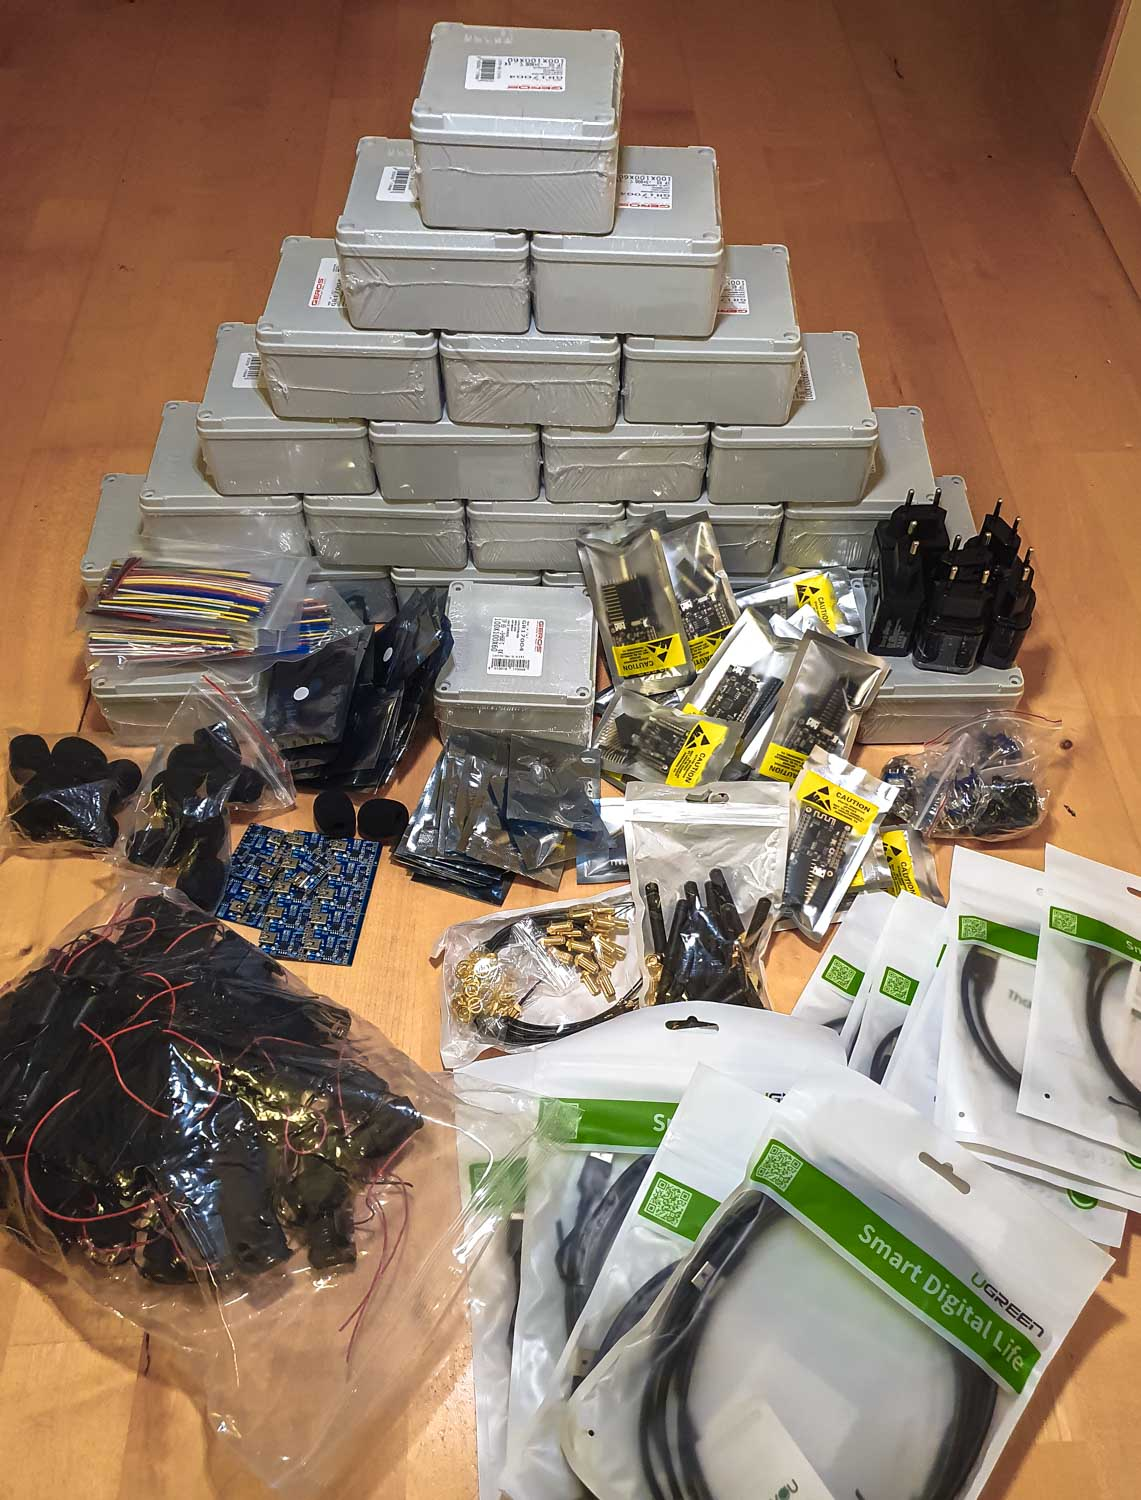
\includegraphics{slikovno_gradivo/inventorij.jpg}


Od prej:


Hrup nas spremlja kamorkoli gremo. Še posebej v mestih in ob prometnih cestah lahko hrup preglasi pogovor, prestraši živali ali celo povzorči neugodna akutna psihična stanja. Dolgoročno pa lahko vpliva na kvaliteto spanja, kar posledično negativno vpliva na koncentracijo in zdravje ljudi ki živijo in se zadržujejo v takšnih okoljih. V zadnijih letih je želja po obvladovanju hrupa sprožila številne projekte. Samo v Ljubljani smo v zadnjih letih omejili promet skozi center in po Slovenski cesti, javni promet je postal bolj dostopen in lažji za uporabo, projekt bicikelj omogoča poceni in hitro izposojo koles. Manj opazen, ampak še zmeraj zelo pomemben pristop obvladovanja hrupa pa je uporaba specifičnih materialov in arhitekturnih praks, ki pomagajo ne le pri zmanjševanju hrupa, ampak tudi pri obvladovanju oblike in tipa hrupa. 

Pri sprejemanju odločitev potrebujemo podatke in s spremljanjem hrupa v različnih delih mesta, kjer so preučevani materiali in prakse že uporabljeni, lahko ugotovimo kakšen vpliv imajo te odločitve na hrup. Ta diplomska naloga se osredotoča na pridobivanje, shranjevanje in upravljanje s podatki. 



\chapter{Tehnologije}
(vsaka črtica tri odstavki, dodaj kakšno sliko, pazi na licence slik, vse mora biti v slovenščini, lahko tudi zrišeš kakšno shemo)

\section{Mikrokontrolerji}



\begin{figure}[H]
    \centering
    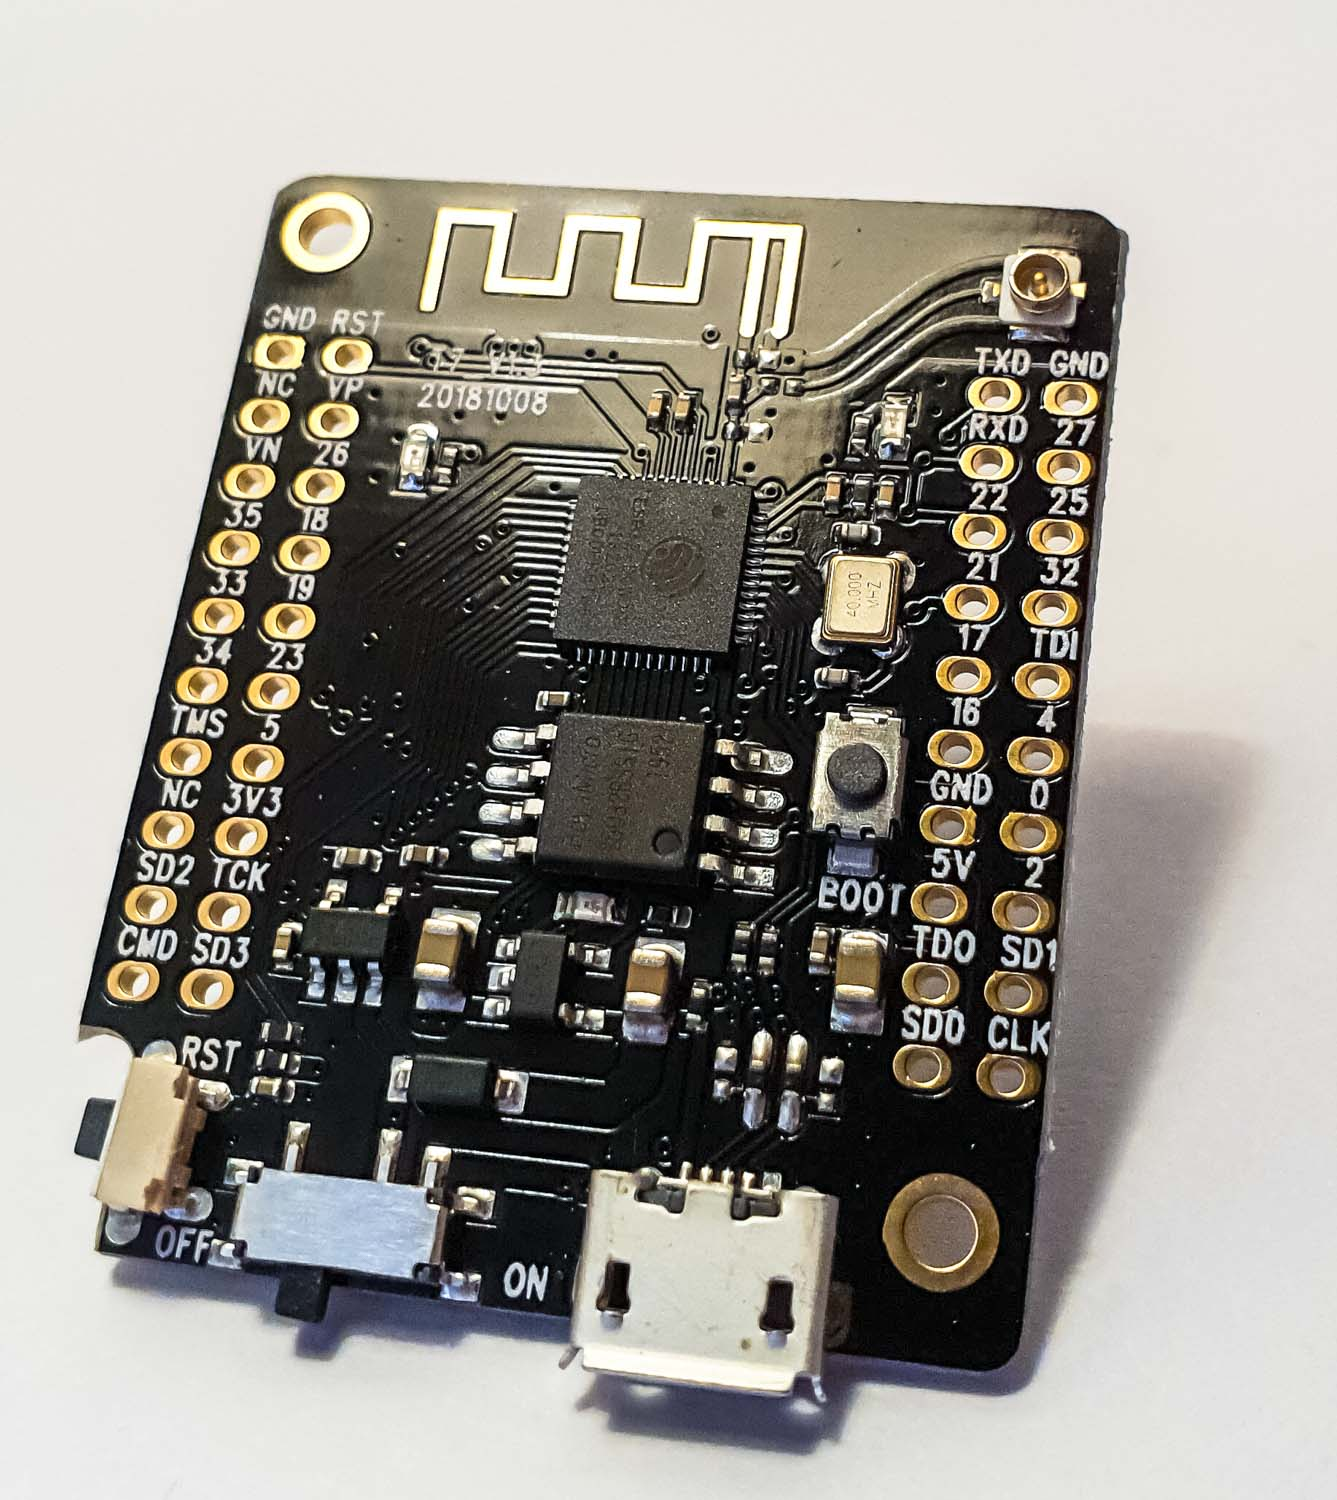
\includegraphics[width=\linewidth]{slikovno_gradivo/ESP32_1.jpg}
    \caption{Razvojna ploščica TTGO T7, ki smo jo upoorabili v merilnih in zbirnih enotah. Izbrali smo jo zaradi majhne porabe energije v načinu spanja in priključkom za zunanjo anteno.}
    \label{fig:TTGO_T7}
\end{figure}


\begin{table}[]
\begin{tabular}{ll}
Ime                                 & ESP32                                                 \\
Proizvajalec                        & Espressif Systems                                     \\
Procesor                            & Tensilica Xtensa LX6 dvojederni + koprocesor          \\
SRAM                                & 512 KiB                                               \\
Možnosti povezovanja                & Wi-Fi 802.11 b/g/n, v4.2 BT + BLE                     \\
Največja moč oddajanja              & 20 dB                                                 \\
Periferne naprave                   & UART, I2C, I2S, SPI, CAN, SD, Ethernet, ADC, DAC, PWM \\
Napajalna napetsot                  & 3.3V                                                  \\
Poraba elektrike                    &                                                       \\
\multicolumn{1}{r}{@240MHz}         & 55mA                                                  \\
\multicolumn{1}{r}{@20MHz}          & 20mA                                                  \\
\multicolumn{1}{r}{Light sleep}     & 0.8mA                                                 \\
\multicolumn{1}{r}{Največja poraba} & 350mA                                                
\end{tabular}
\caption{Pregled lastnosti mikrokontrolerja ESP32.}
\label{fig:esp32_spec}
\end{table}
MIkrokontrolerji so ena najmanjših oblik računalnikov. Uporabljajo se v skoraj vseh elektronskih napravah. Veliko naprav ima več mikrokontrolerjev. 
Rešujejo od najbolj osnovnih problemov kot so polnenje baterij do zelo zahtevnih in kritičnih operacij kot so zaviralni sistemi v avtomobilu in razne avtonomne postaje.
Projekt Arduino je mladim programerjem in raziskovalcem približal delo z mikrokontrolerji, tako da so zaradi manjše začetne cene in lahkim razvojem vedno bolj populrani  

\section{Merjenje hrupa (senzorji)}



\begin{figure}[H]
    \centering
    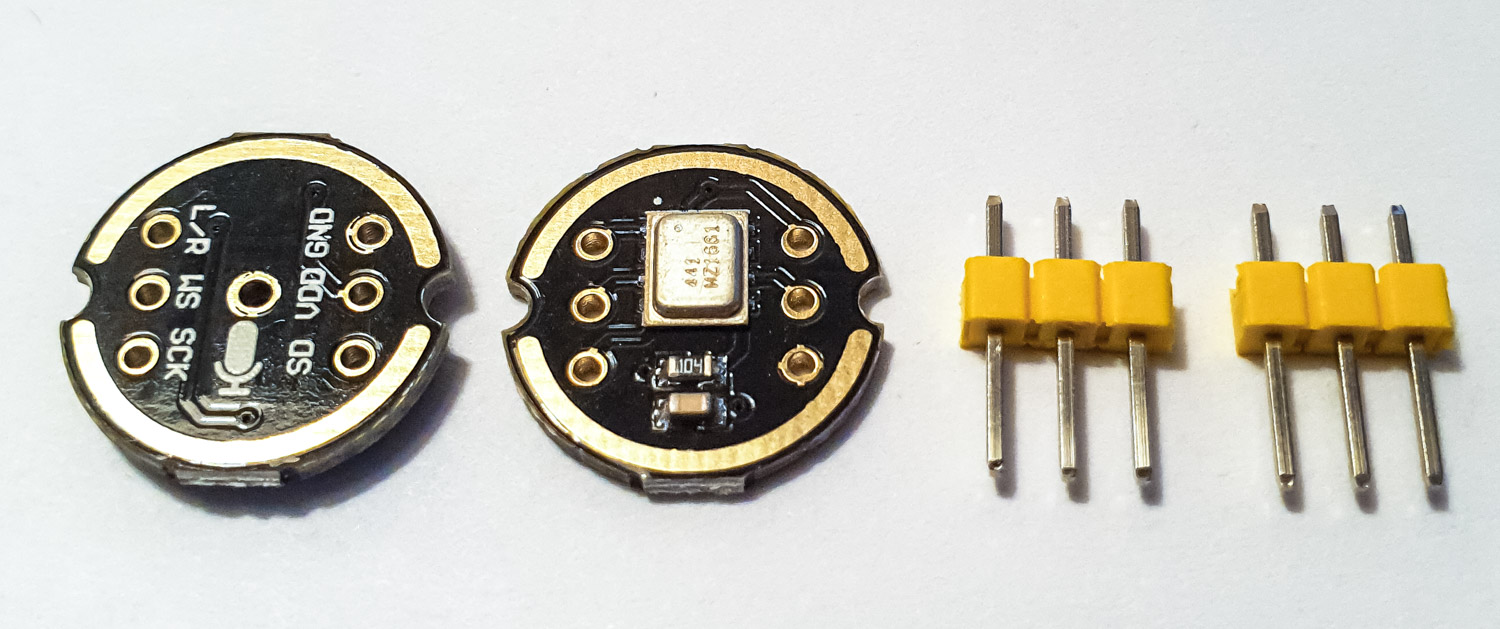
\includegraphics[width=\linewidth]{slikovno_gradivo/INMP441_1.jpg}
    \caption{Mikrofon INMP441 na svoji ploščici za lažji dostop do kontaktov.}
    \label{fig:INMP441}
\end{figure}


\begin{figure}[H]
    \centering
    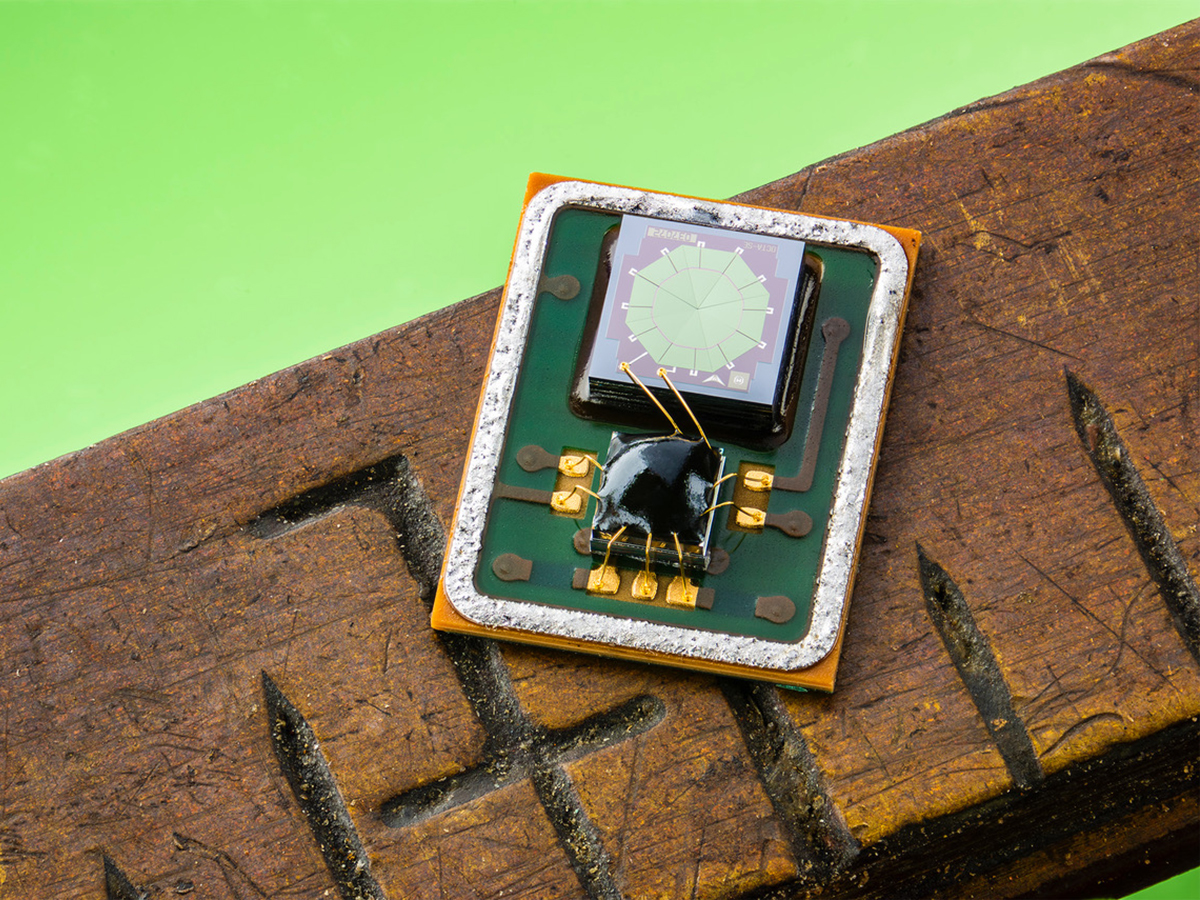
\includegraphics[width=\linewidth]{slikovno_gradivo/mems-mic2.jpg}
    \caption{Na sliki so jasno razvidni glavni deli MEMS mikrofona.}
    \label{fig:mems_mic}
\end{figure}


\begin{table}[]
\begin{tabular}{l|l}
Ime                                        & INMP441        \\
Proizvajalec                               & InvenSense     \\
Protokol                                   & 24bit I2S      \\
Razpon frekvence vzorčenja                 & 7.8kHz - 50kHz \\
Frekvenčni razpon                          & 60Hz - 15kHz   \\
Napajalna napetsot                         & 3.3V           \\
Poraba elektrike                           &                \\
\multicolumn{1}{r}{Aktivno stanje}         \vline & 2.2mA          \\
\multicolumn{1}{r}{Stanje pripravljenosti} \vline & 0.8mA          \\
\multicolumn{1}{r}{Spanje}                 \vline & 0.0045mA      
\end{tabular}
\caption{SPecifijkacije izbranega INMP441 mikrofona.}
\label{tbl:IMP441_spec}
\end{table}

Svojevrsten tehnološki čudež so MEMS naprave. Pod to spadajo tudi MEMS mikrofoni, ki smo jih uporabili pri zajemanju podatkov. Ti mikrofoni imajo že vgrajene pretvornike iz analognega v digitalni signal. Ker gre za tehnologijo, ki je podobna izdelavi procesorskih čipov, so lahko razlike med enotami precej manjše od navadnih mikrofonov. Te mikrofone odlikuje tudi zelo majhna poraba in izredno majhna fizična velikost.

\section{Povezljivost}


\begin{table}[H]
\begin{tabular}{l|llll}
                & ESPNOW                                                                                                                          & NRF24                                                                                                                                                                                          & LoRa                                                                                                        & WiFi                             \\ \hline
Doseg           & 100m-1km                                                                                                                        & 100m-1km                                                                                                                                                                                       & 1km-10km                                                                                                    & 10m-100m                         \\
Hitrost prenosa & 250kbps                                                                                                                         & 250kbps                                                                                                                                                                                        & 300bps-19kbps                                                                                               & 1mbps-150mbps                    \\
Poraba energije & 100mA                                                                                                                           & 100mA                                                                                                                                                                                          & 30mA                                                                                                        & 150mA                            \\
Posebnosti      & \begin{tabular}[c]{@{}l@{}}- naslavljanje preko MAC naslovo\\ - ni omrežne plasti \\ - omejena na ESP32 in ESP8266\end{tabular} & \begin{tabular}[c]{@{}l@{}}- doseg je zelo odvisen od kvalitete modulov\\ - poleg mikrokontrolerja bi potrebovali še en modul\\ - zelo okoren za obvladovanje več naprav naenkrat\end{tabular} & \begin{tabular}[c]{@{}l@{}}- prenos podatkov je precej prepočasen\\ - potrebuje mikrokontroler\end{tabular} & - zelo velik overhead            \\
Cena            & Samo cena ESP32 mikrokontrolerja                                                                                                & Mikrokontroler plus 4€ za kvaliteten NRF24 modul                                                                                                                                               & Mikrokontroler plus 10€ za LoRa                                                                             & Samo cena ESP32 mikrokontrolerja
\end{tabular}

\caption{Ne znam narest  tega tukej lepš}
\label{tbl:primerjava_povezljivosti}
\end{table}


\begin{figure}[H]
    \centering
    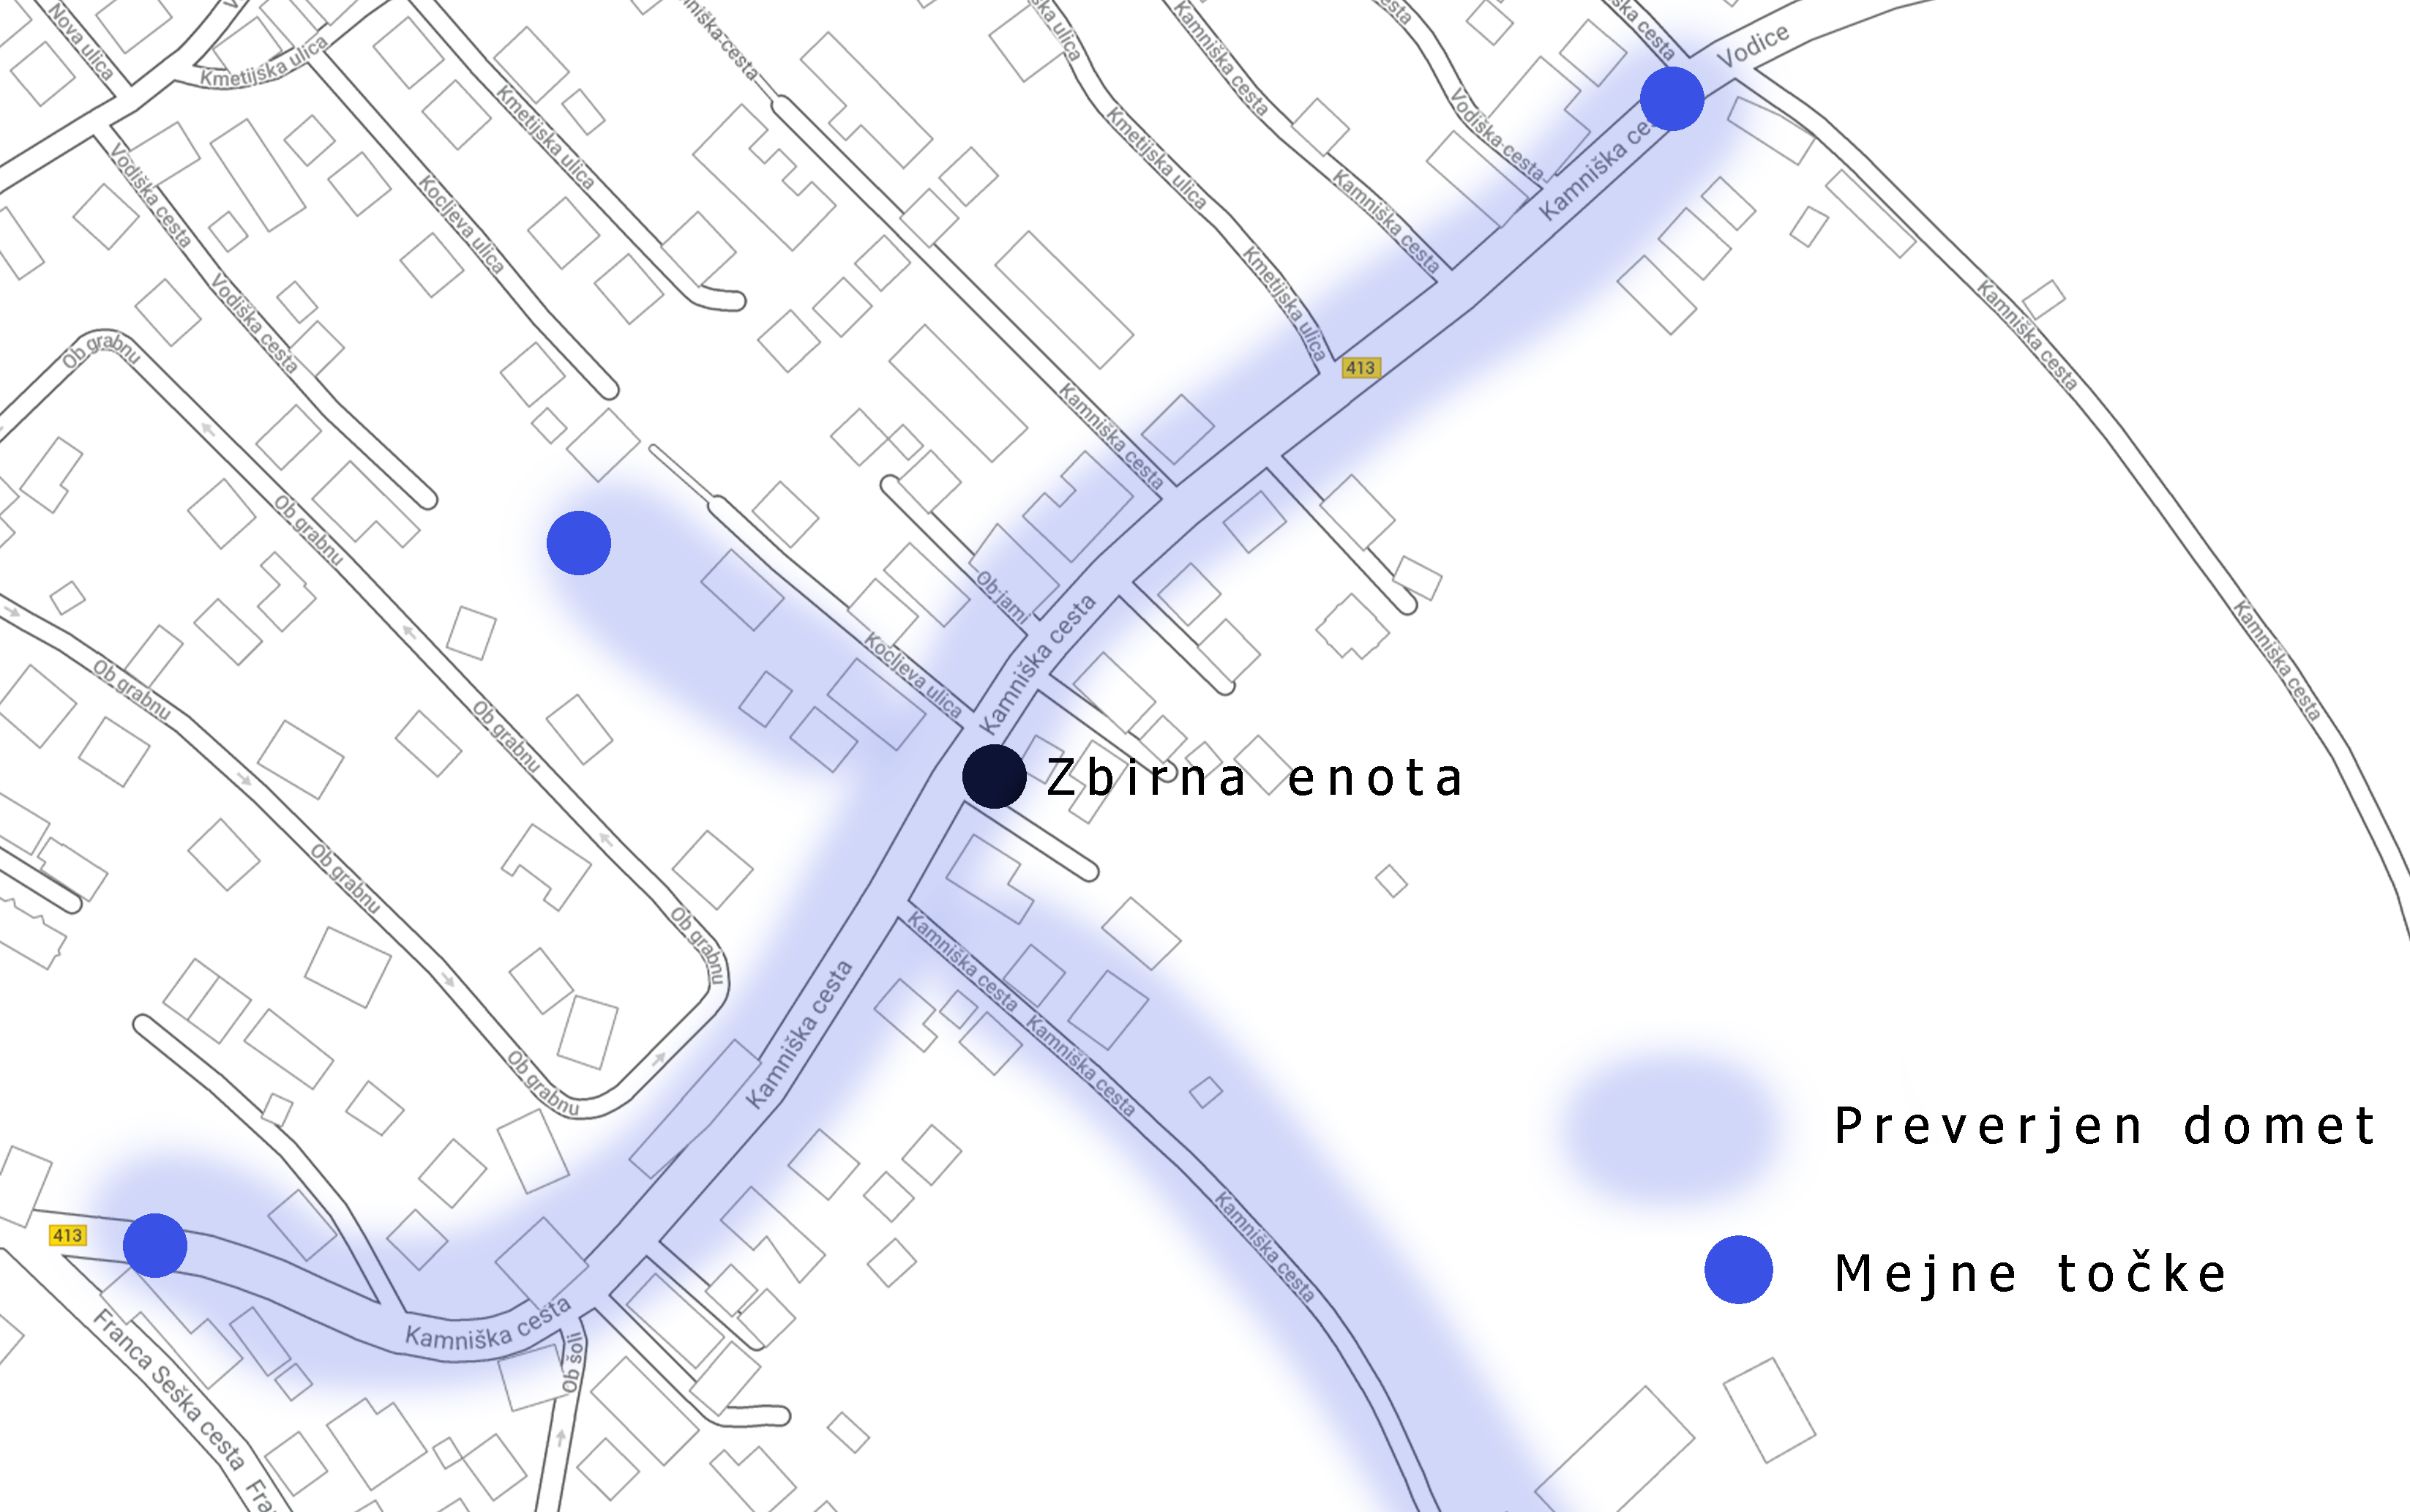
\includegraphics[width=\linewidth]{slikovno_gradivo/Domet.png}
    \caption{Prikaz testiranega dometa v urbanem okolju. Oddaljenost mejnih točk od zbirne točke je 250m, 157m in 270m. Testiranje na prostem je ob optimalnih pogojih pokazalo domet do 1500m.}
    \label{fig:INMP441}
\end{figure}

Moderni mikrokontrolerji omogočajo precej različnih možnosti povezovanja. Najbolj razširjeni so protokoli wifi, ble, lora in NRF24. Pri odločanju med temi protokoli smo iskali optimalno mešanico cenovne ugodnosti, dosega povezave, hitrosti povezave in majhne porabe energije. (tabela s podatki o teh tehnologijah).

\section{Programska oprema za IOT}

* tabela prednosti in slabosti razisskani opcij

\section{Strežniški del}

NodeJS? tudi tu ne vem točno kaj in kako 

\chapter{Rešitev}
\section{Uporabniške zahteve}
(detaljne zahteve, lahko jih spišeš po sklopih)

Zasnovo in implementacijo sistema smo temeljili na dobri uporabniški izkušnji. Zahteve so bile:
- intuitivno in gospodarno upravljanje s senzorji in zbirniki
- Pregled nad stanjem in lokacijo senzorjev
- Razdelitev podatkov v smiselne zaključene enote
- Uporabne poizvedbe po podatkih, za potrebe podatkovne analitike
- Točni in čim bolj polni podatki o hrupu 


\section{Arhitektura}
(nujno shema)


\begin{figure}[H]
    \centering
    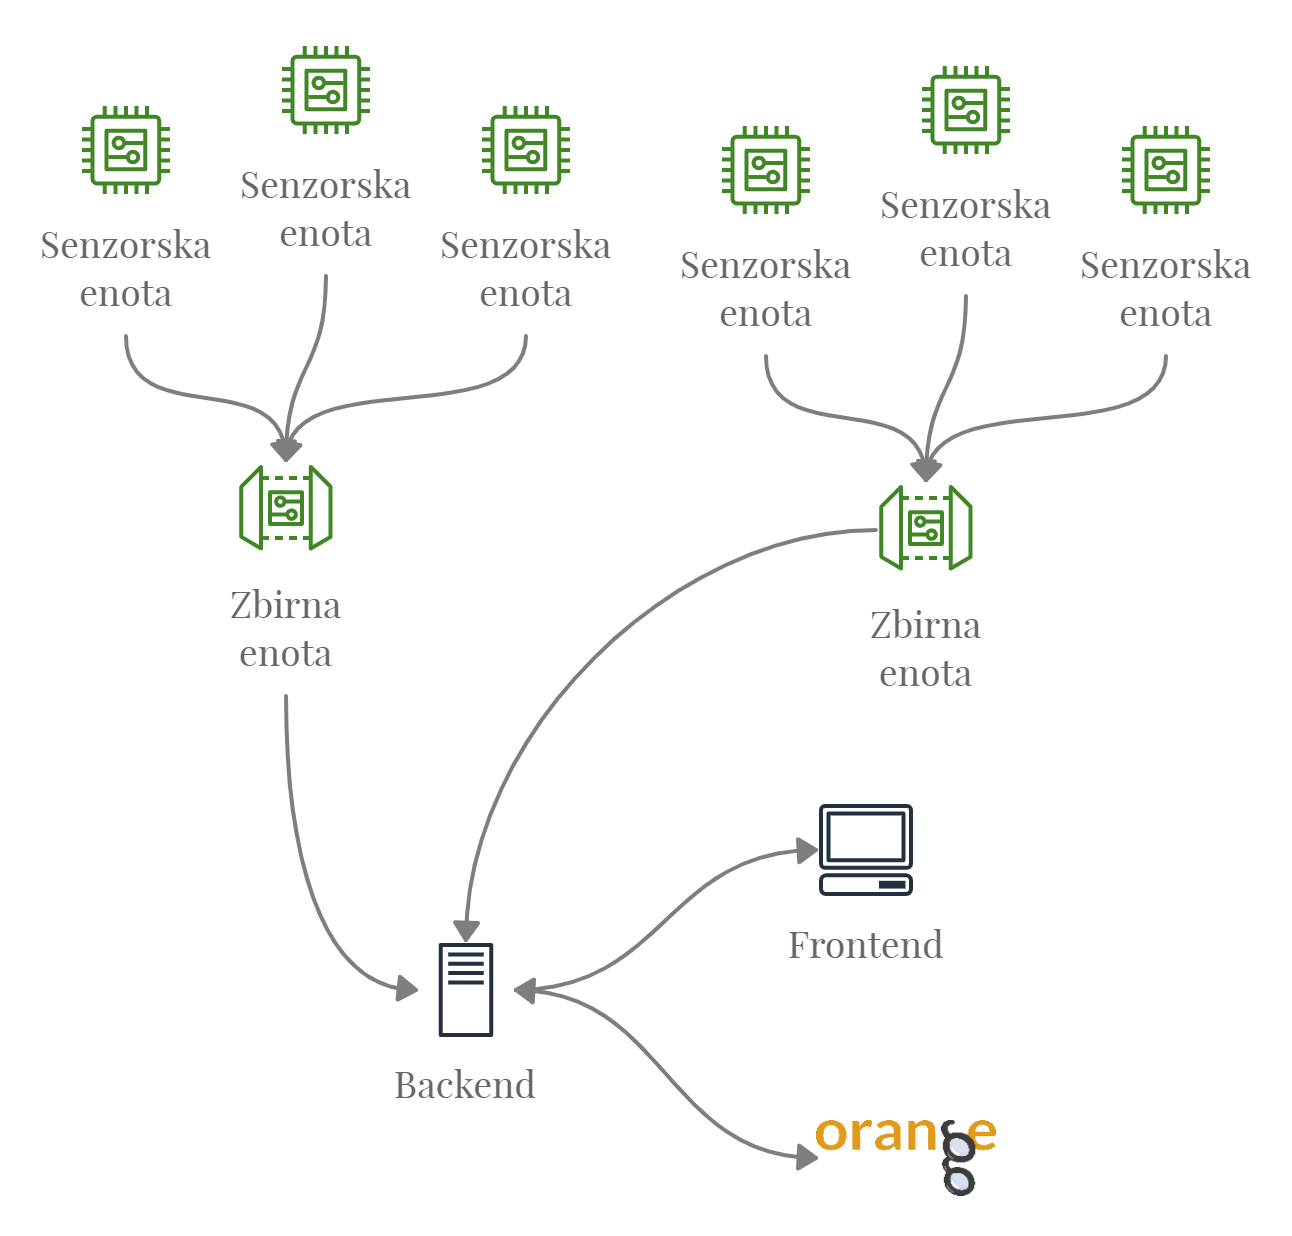
\includegraphics[width=\linewidth]{slikovno_gradivo/Shema celote arhitekture (2).png}
    \caption{Shema implementirane strukture celotnega sistema.}
    \label{fig:arhiterktura}
\end{figure}
* shema posameznih delov z oblikami sporočil ki se prenašajo med deli
\begin{figure}[H]
    \centering
    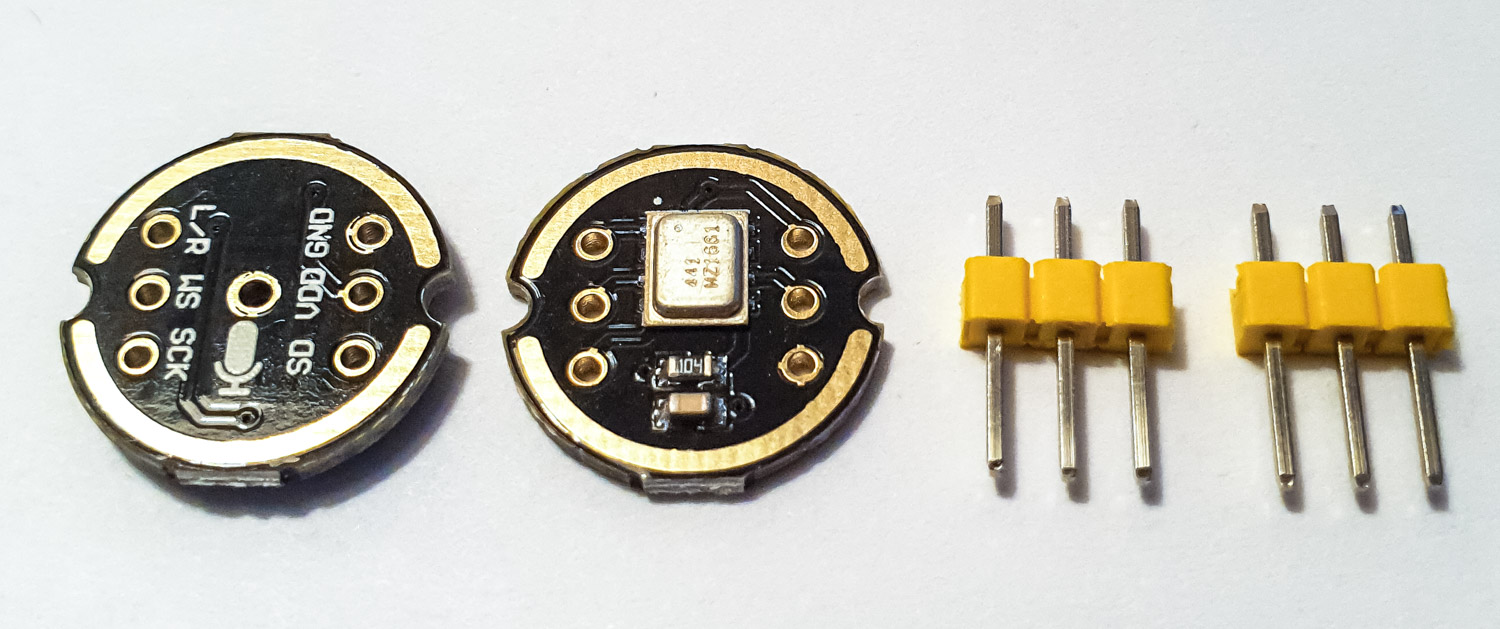
\includegraphics[width=\linewidth]{slikovno_gradivo/INMP441_1.jpg}
    \caption{Caption}
    \label{fig:INMP441}
\end{figure}

Projekt je zasnovan večnivosjsko. Uporabljen je bil princip MVC z dodatkom fizičnih naprav za zajemanje podatkov. Na zalednem delu shranjujemo podatke v bazi mongoDB, ki nam omogoča veliko izbire pri snovanju agregacij podatkov in shranjevanja podtakov v uporabne strukture, ki omogočajo lažji razvoj in hitrejše delovanje sistema. 

Podatke s senzorjev in iz uporabniškega vmesnika sprejema in dostavlja strežnik, zasnovan s tehnologijo NodeJS. Odprtih ima več API podatkovnih dostopnih točk (joj ne spomnm se bolše besede), hkrati pa skrbi za dostavo spletnega uporabniškega vmsenika. 

Uporabniki in skrbniki lahko s sistemom upravljajo preko spletnega vmesnika, ki omogoča pregled nad deploymenti, predgled nad stanjem senzorjev, ustvarjanjem nobvih deploymentov in osnovnim pregledom nad podatki.

Koncept zajemanje in pošiljanje podatkov smo zasnovali na principu topologije zvezde, ki je že precej uveljavljen v industriji iot rešitev in internetu na splošno. Več senzorjev pošilja podatke na eno zbirno enoto, ki jih preko internetne povezave posreduje zalednemu delu.

Podtakovno analizo smo končnemu uporabniku omogočili z implementacijo widgeta, v kontekstu programa za podtakovno znanost Orange. Možnih je več različnih agregacij podatkov.



\section{Merilna enota}


\begin{figure}[H]
    \centering
    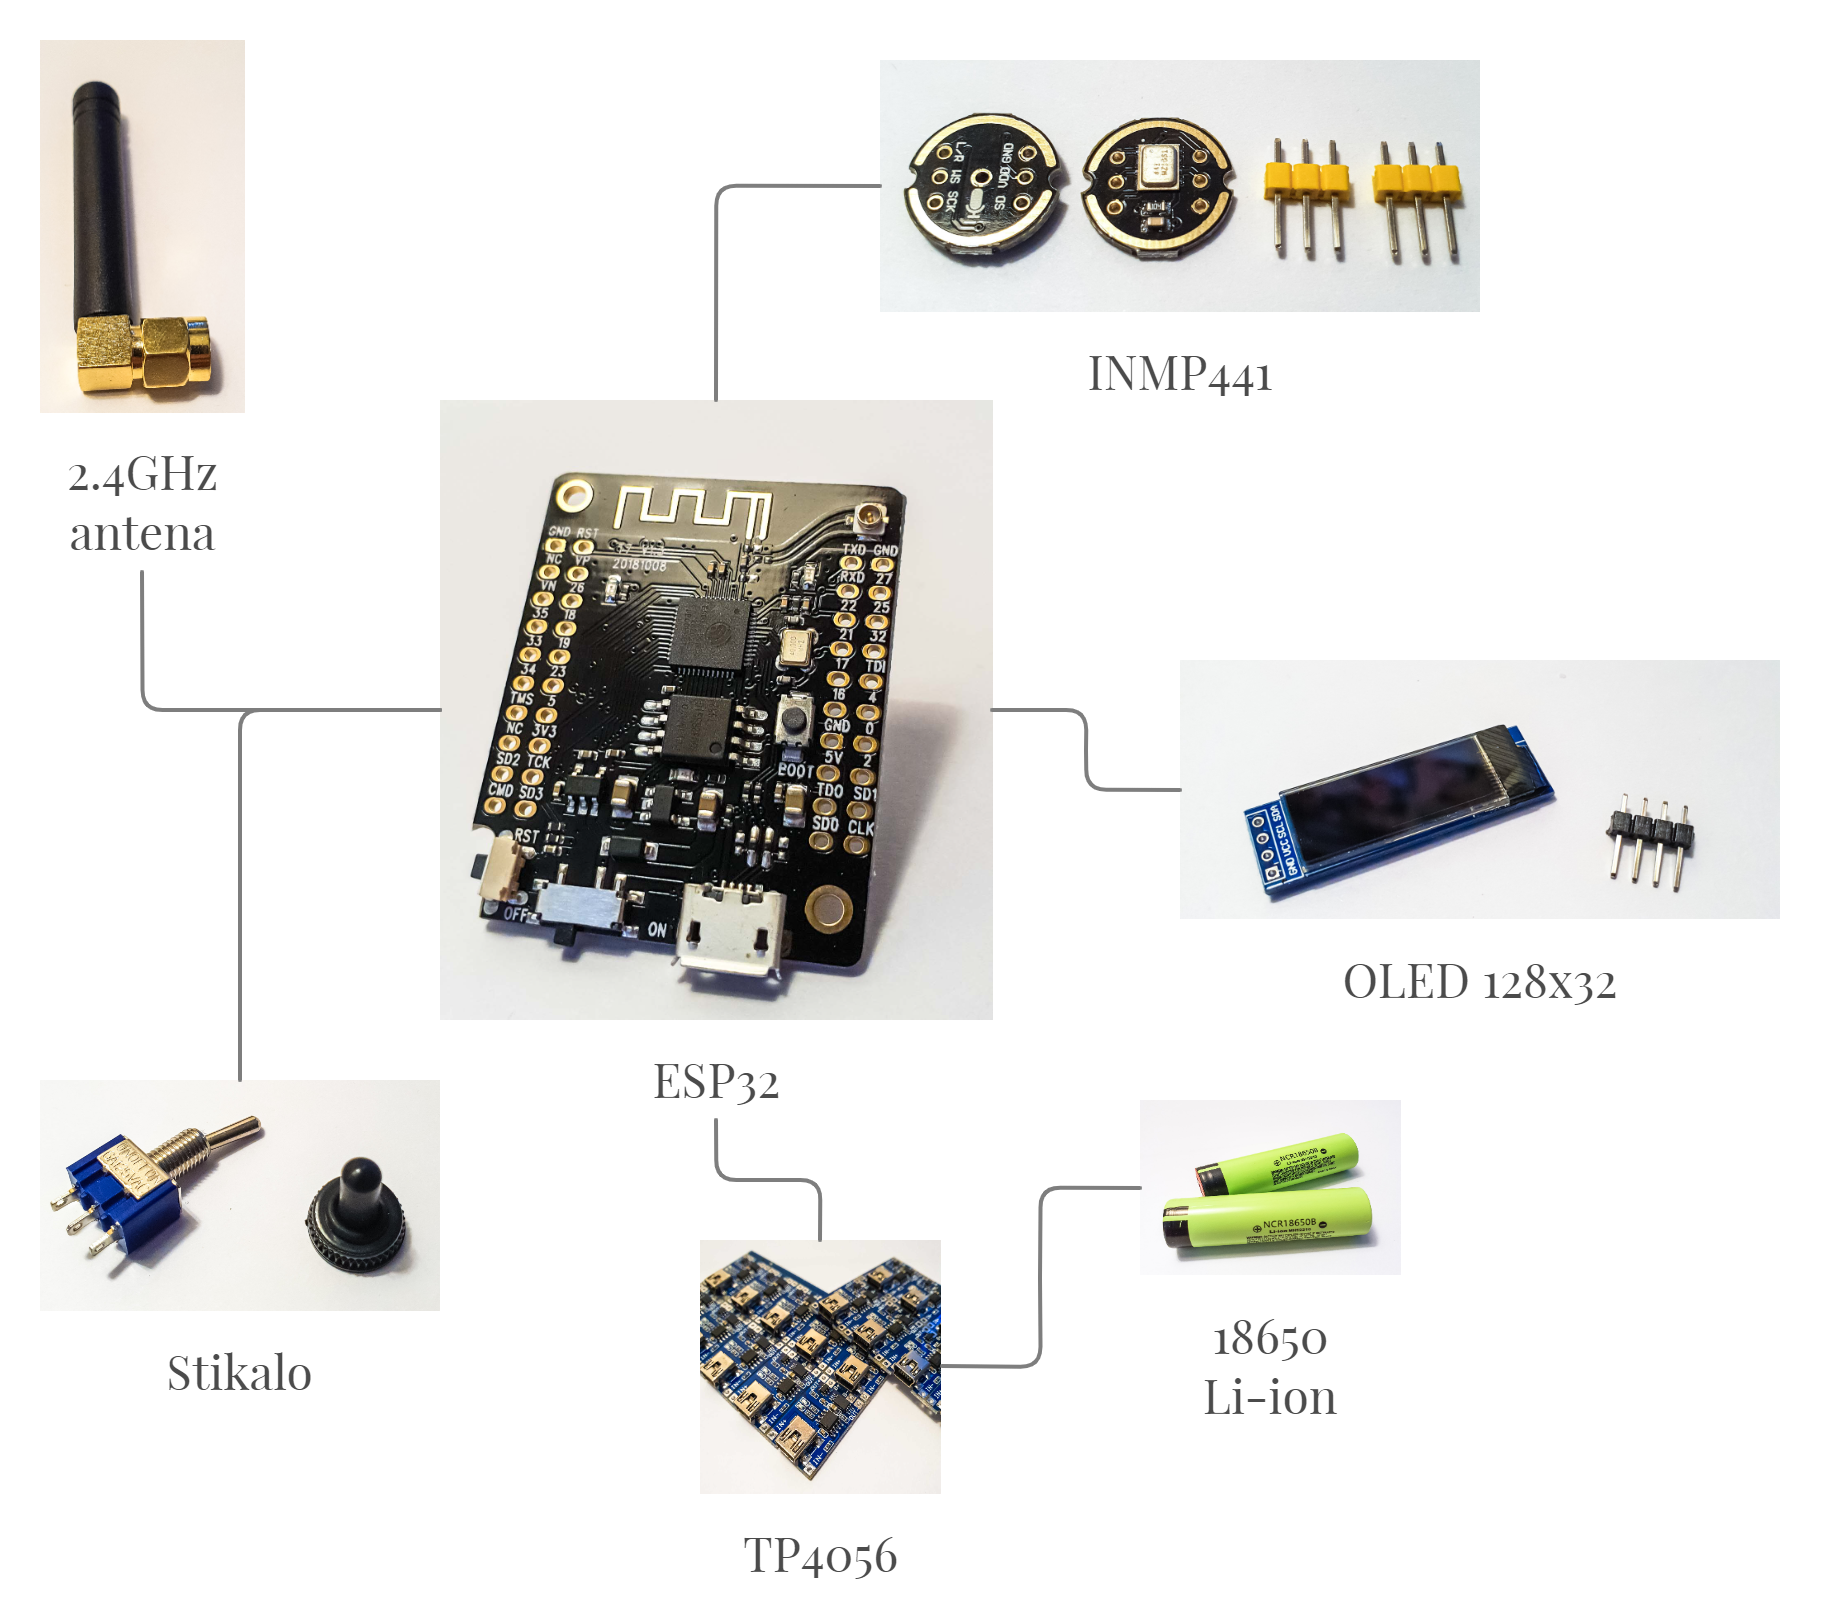
\includegraphics[width=\linewidth]{slikovno_gradivo/Konceptualna shema merilne enote (2).png}
    \caption{Shematski prikaz merilne enote. S črtami so označene električne povezave med deli.}
    \label{fig:shema_merilna}
\end{figure}

\begin{figure}[H]
    \centering
    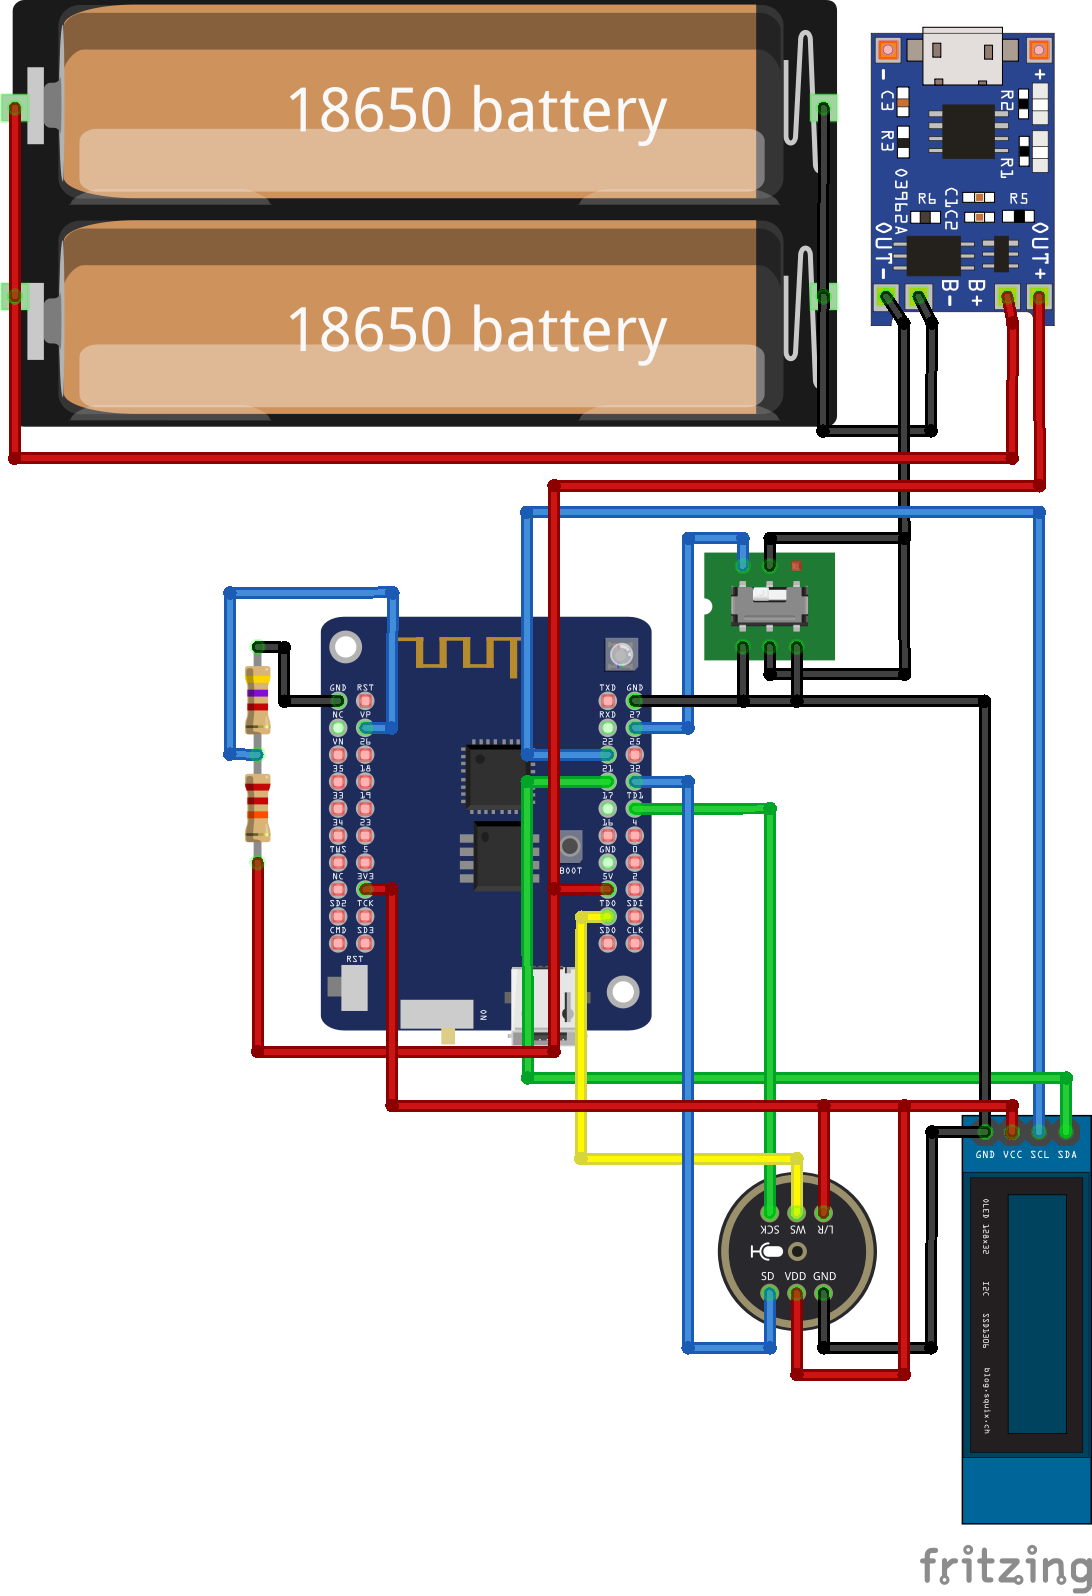
\includegraphics[width=\linewidth]{slikovno_gradivo/merilna_enota_bb.png}
    \caption{Caption}
    \label{fig:INMP441}
\end{figure}


\begin{figure}[H]
    \centering
    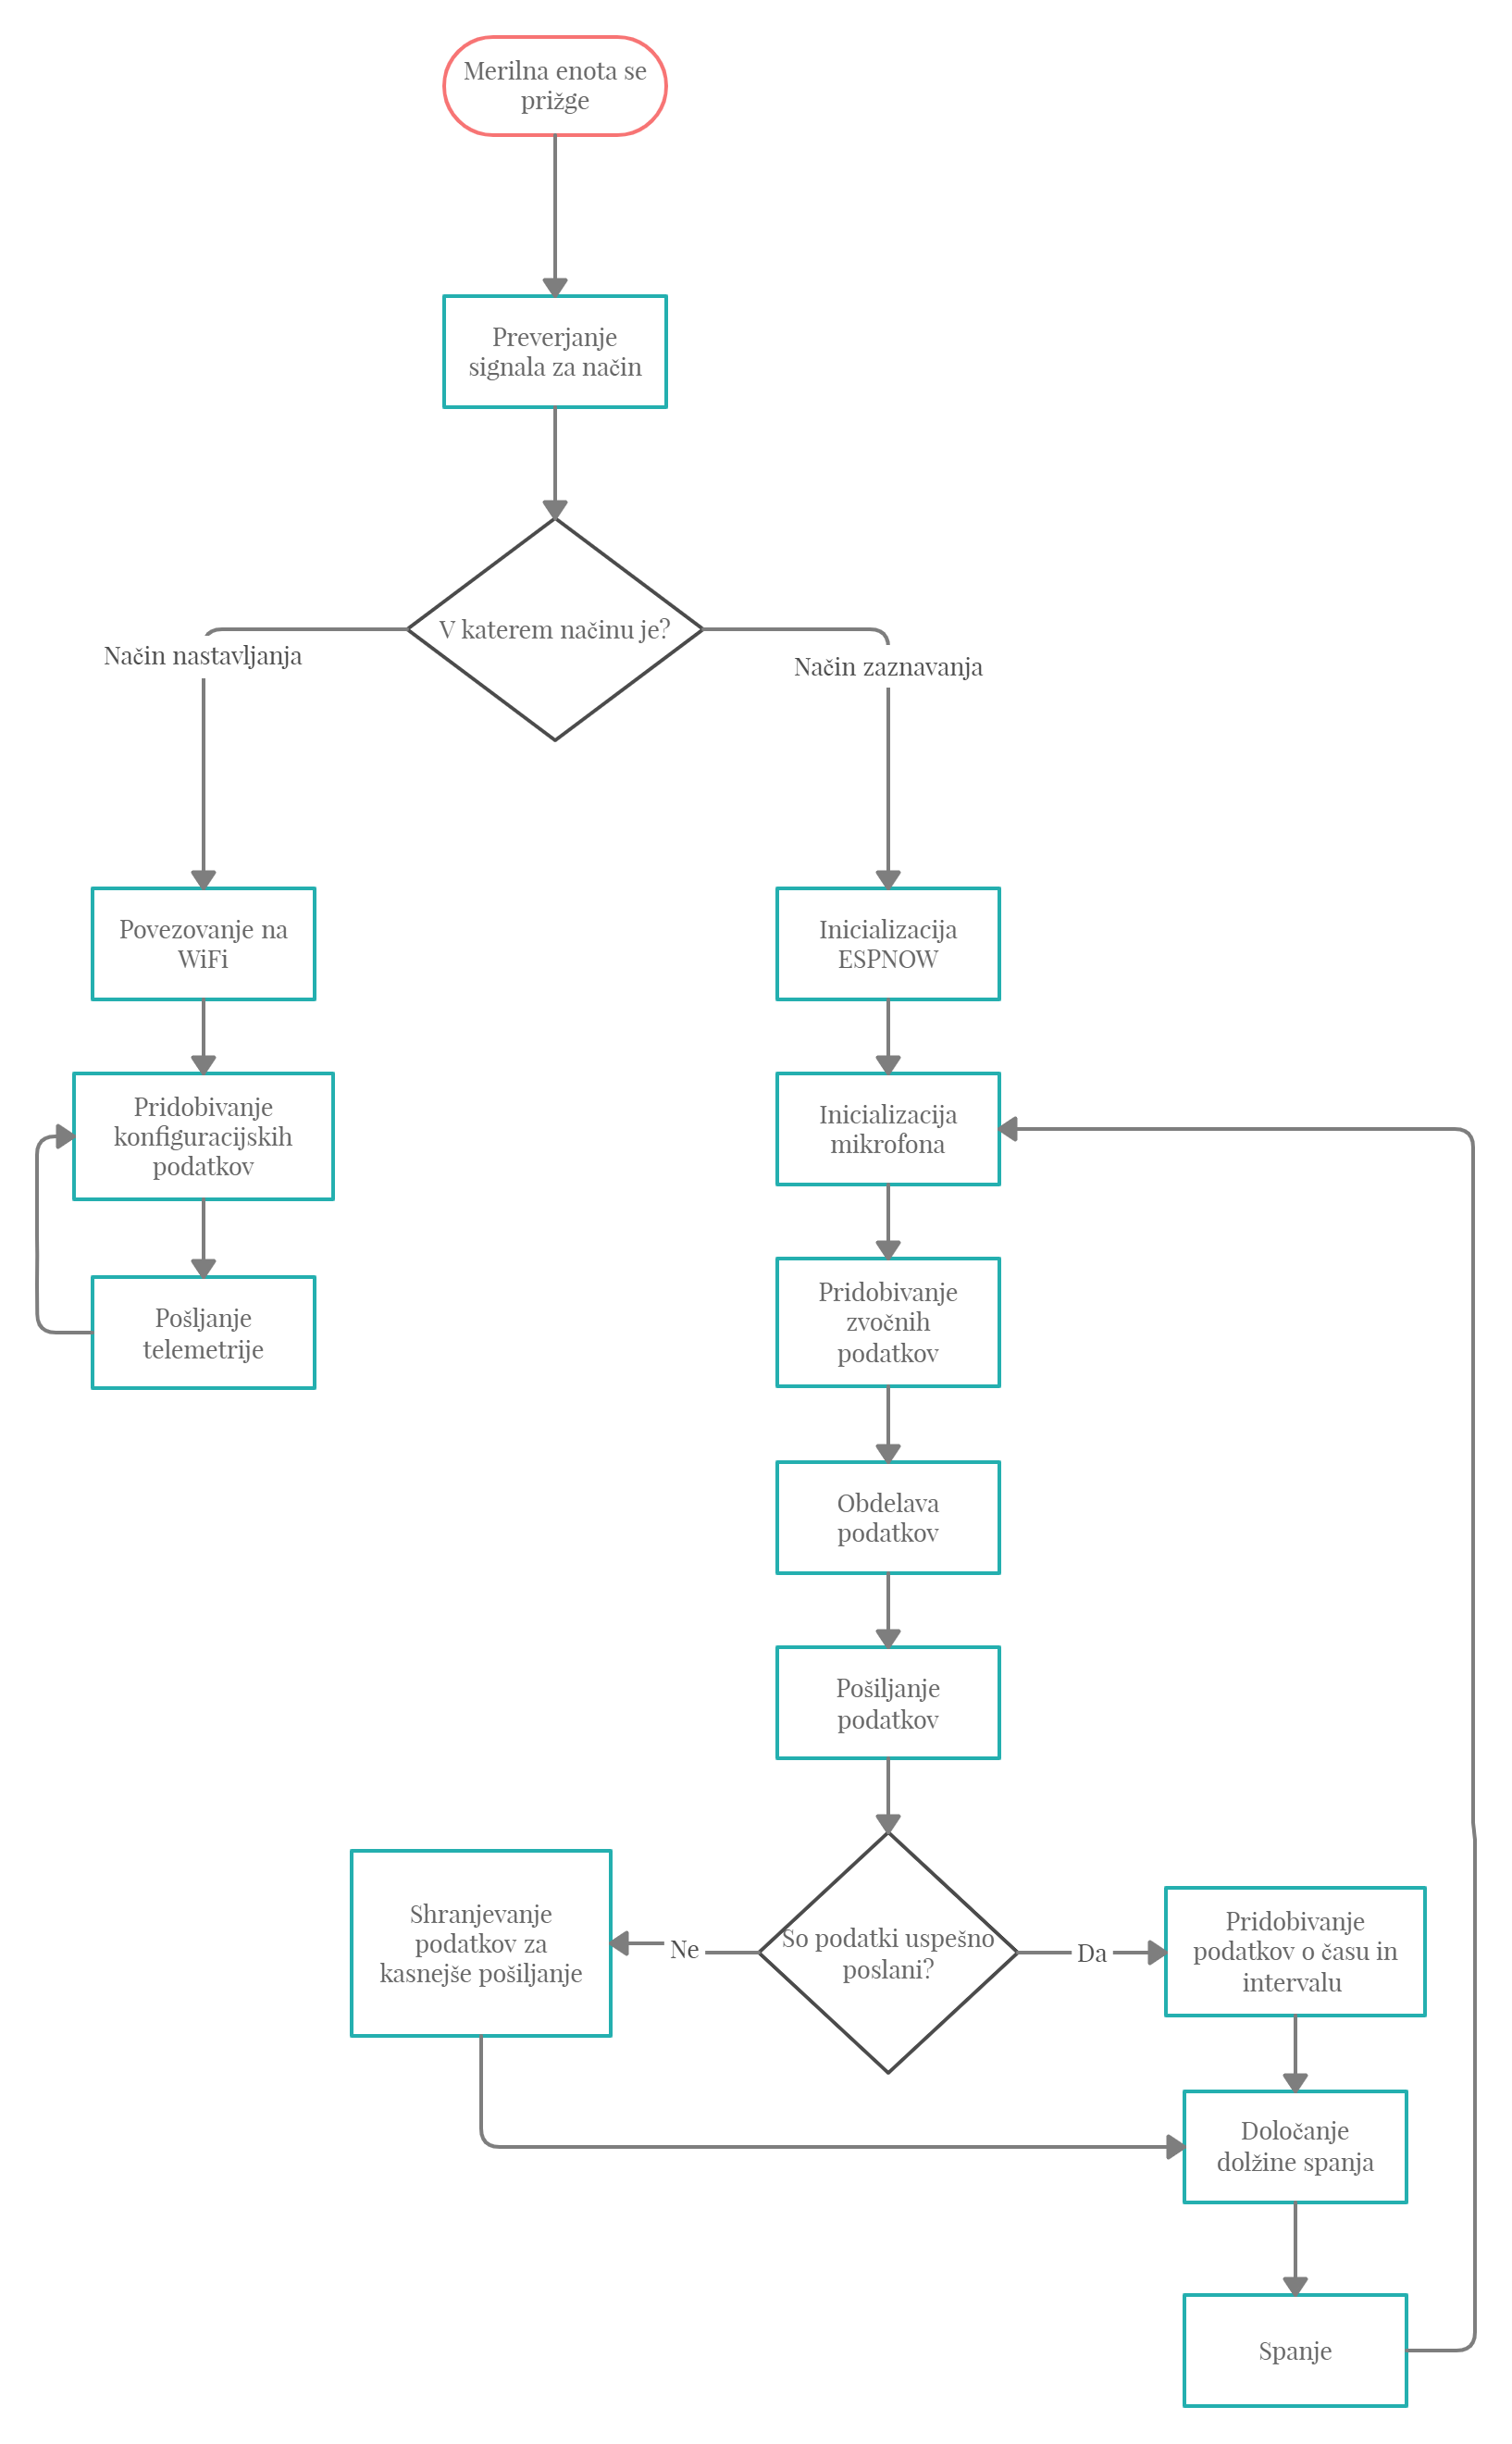
\includegraphics[width=\linewidth]{slikovno_gradivo/Merilna enota delovanje (1).png}
    \caption{Prikaz obeh načinov delovanja merilne enote. Način delovanja je določen S stikalom, ki ob zagonu enote določi v katerem načinu bo enota delovala. V načinu za nastavljanje pridobi podatke o delovanju s strežnika in počija svojo telemetrijo, v načinu zaznavanja pa enota zajame podatke o zvoku, jih obdela in jih periodično pošilja na zbirno enoto.}
    \label{fig:potek_mmerilna}
\end{figure}

\begin{figure}[H]
    \centering
    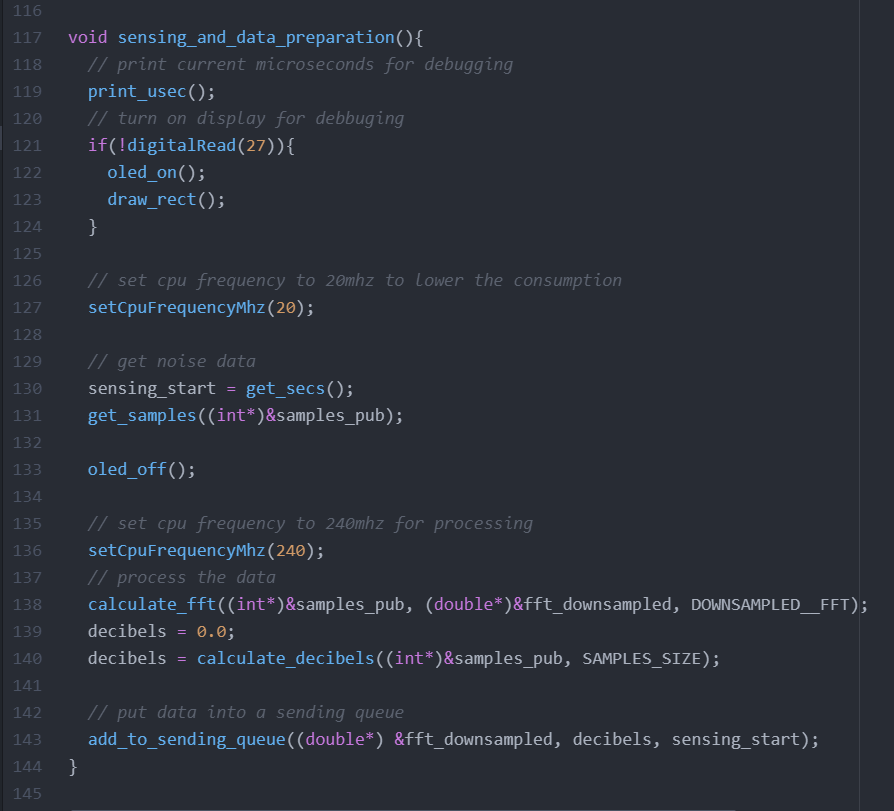
\includegraphics[width=\linewidth]{slikovno_gradivo/koda_podatki.png}
    \caption{Programska koda, ki se izvede ob vsakem merjenju hrupa.}
    \label{fig:koda_podatki}
\end{figure}
* fotografija enote

\begin{figure}[H]
    \centering
    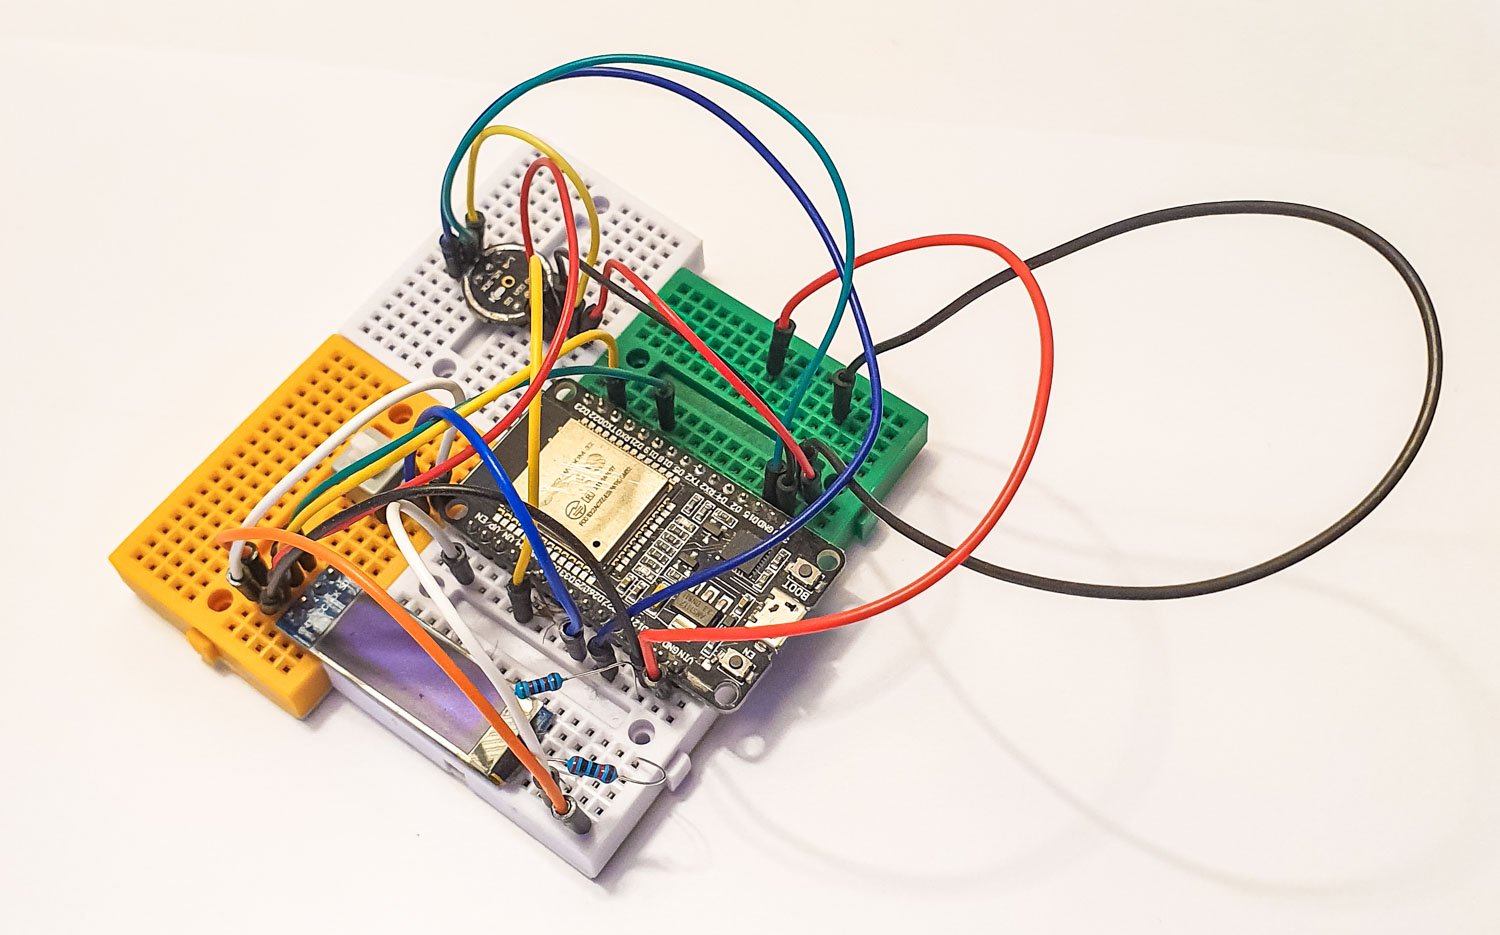
\includegraphics[width=\linewidth]{slikovno_gradivo/prototip_1.jpg}
    \caption{Eden od prototipov merilne enote namenjenih zaa razvoj programske opreme, testiranje dometa in porabe energije.}
    \label{fig:prototip}
\end{figure}


\begin{figure}[H]
    \centering
    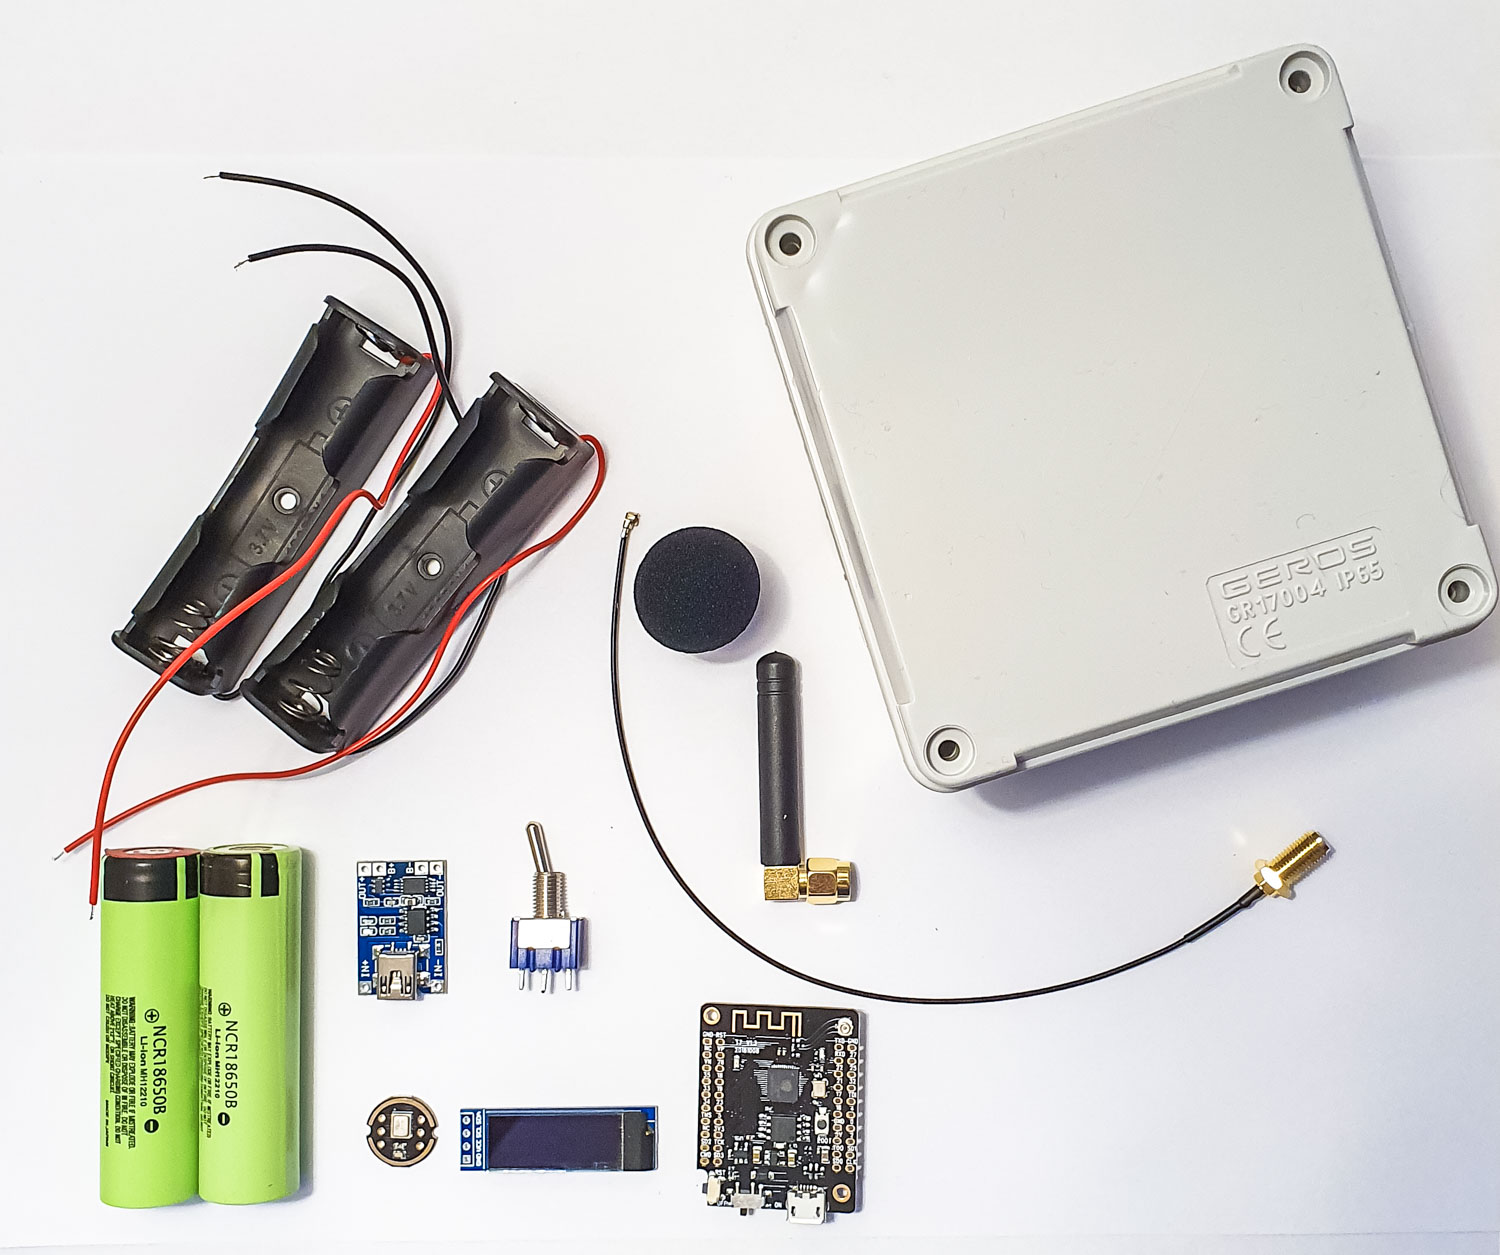
\includegraphics[width=\linewidth]{slikovno_gradivo/merilna_enota_2.jpg}
    \caption{Fotografija materiala za vsako merilno enoto.}
    \label{fig:material_merilna}
\end{figure}


Pri zasnovi merilne enote smo se spopadli s specifičnimi zahtevami, ki so močno vplivale na odločitve pri implementaciji.

Glavni del merilne enote je mikrokontroler ESP32, ki omogoča več načinov brezžične komiunikacije z zadovoljivo dolgim dosegom. 
Pri izbiri komunikacijskega portokola smo bili pozorni na overhead, ki mora biti zaradi strogih zahtev po majhni porabi energije čim manjši. Odločili smo se za uporabo ESPNOW. Na fizičnem nivoju je ta protokol isti kot wifi, ima pa prednost daljšega dometa in pošiljanje podatkov brez vzpostavljanja povezave. 

Za napajanje smo uporabili dve 18650 li ion bateriji, ki naj bi napajali napravo vsaj en mesec. 

Pri izbiri mikrofona smo se zaradi lažjega sestavljanja in majše cene omejli samo na mikrofone, ki so že montirani na svojih ploščicah z dostopnimi kontakti za podatke in napajanje.

Ekran je vključen za lažje prepoznavanje napak in nastavljanje.

Za lažje uporavljanje merilnih enot, smo implementirali dva načina delovanja med katerima lahko preklapljamo s stikalom. 
Ko je enota v načinu za uporavljanju, se poveže na specifično wifi omrežje, se registrira v sistem in dobi podatke, ki jih potrebuje za zaznavanje in pošiljanje podtakov. Na ekranu se izpišujejo ime te enote in trenutni podatki o zvoku.
Način za zaznavanje in pošiljanje podatkov zbudi enoto iz spanja, zbere podatke o zvoku, jih pošlje na zbirno enoto in od zbirne enote zahteva signal za časovno sinhronizacijo.




\section{Zbirna enota}



\begin{figure}[H]
    \centering
    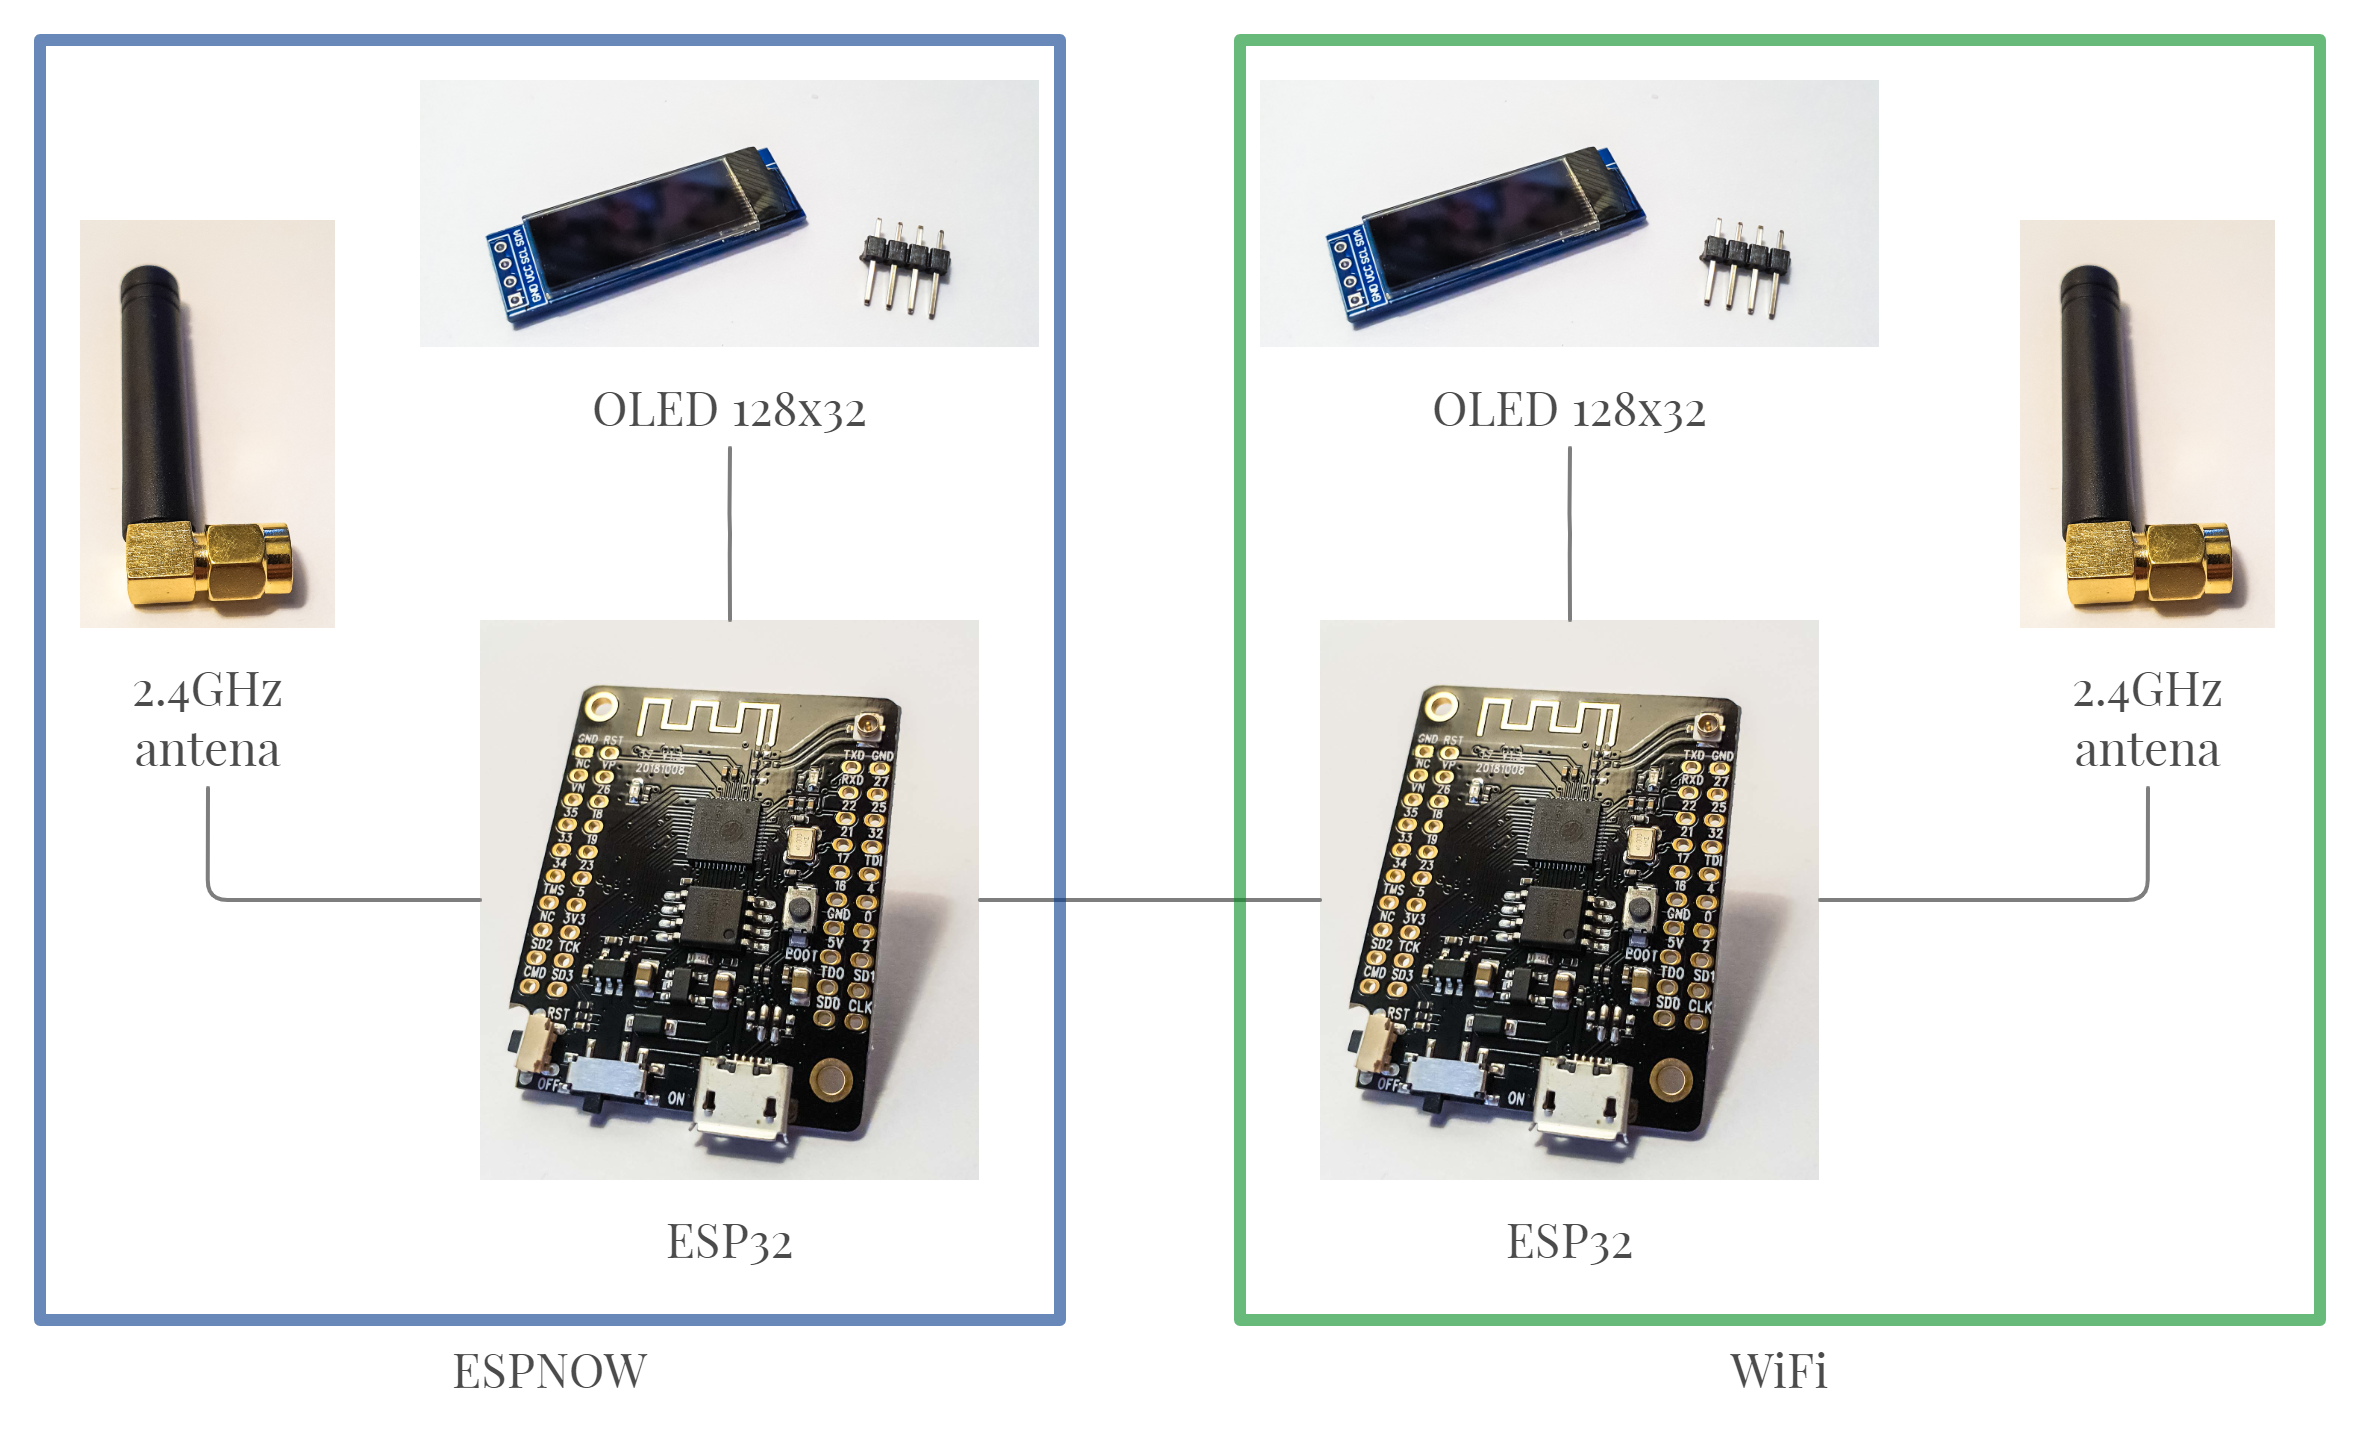
\includegraphics[width=\linewidth]{slikovno_gradivo/Zbirna enota shematski prikaz.png}
    \caption{Na sliki je prikazan shematski prikaz zbirne enote z vrisanimi električnimi in podatkovnimi povezavami. Jasno je razvidna tudi razlika med WiFi in ESPNOW dellom.}
    \label{fig:shema_zbirna}
\end{figure}


\begin{figure}[H]
    \centering
    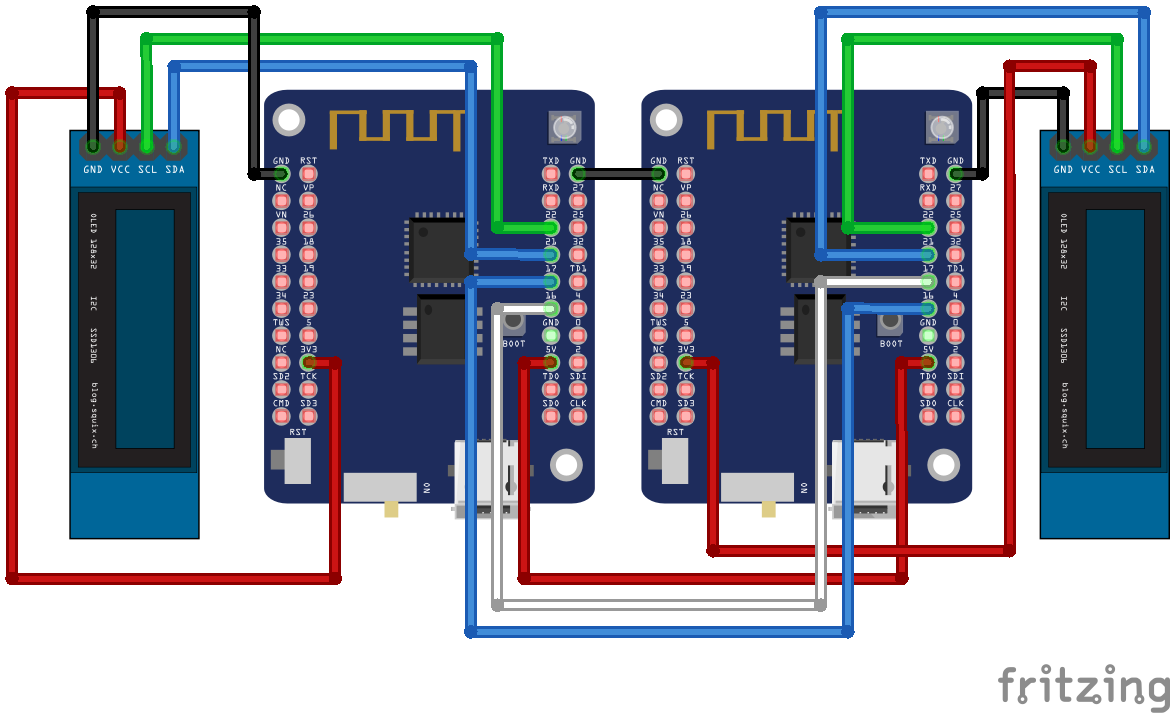
\includegraphics[width=\linewidth]{slikovno_gradivo/zbirna_enota_bb.png}
    \caption{Caption}
    \label{fig:INMP441}
\end{figure}


\begin{figure}[H]
    \centering
    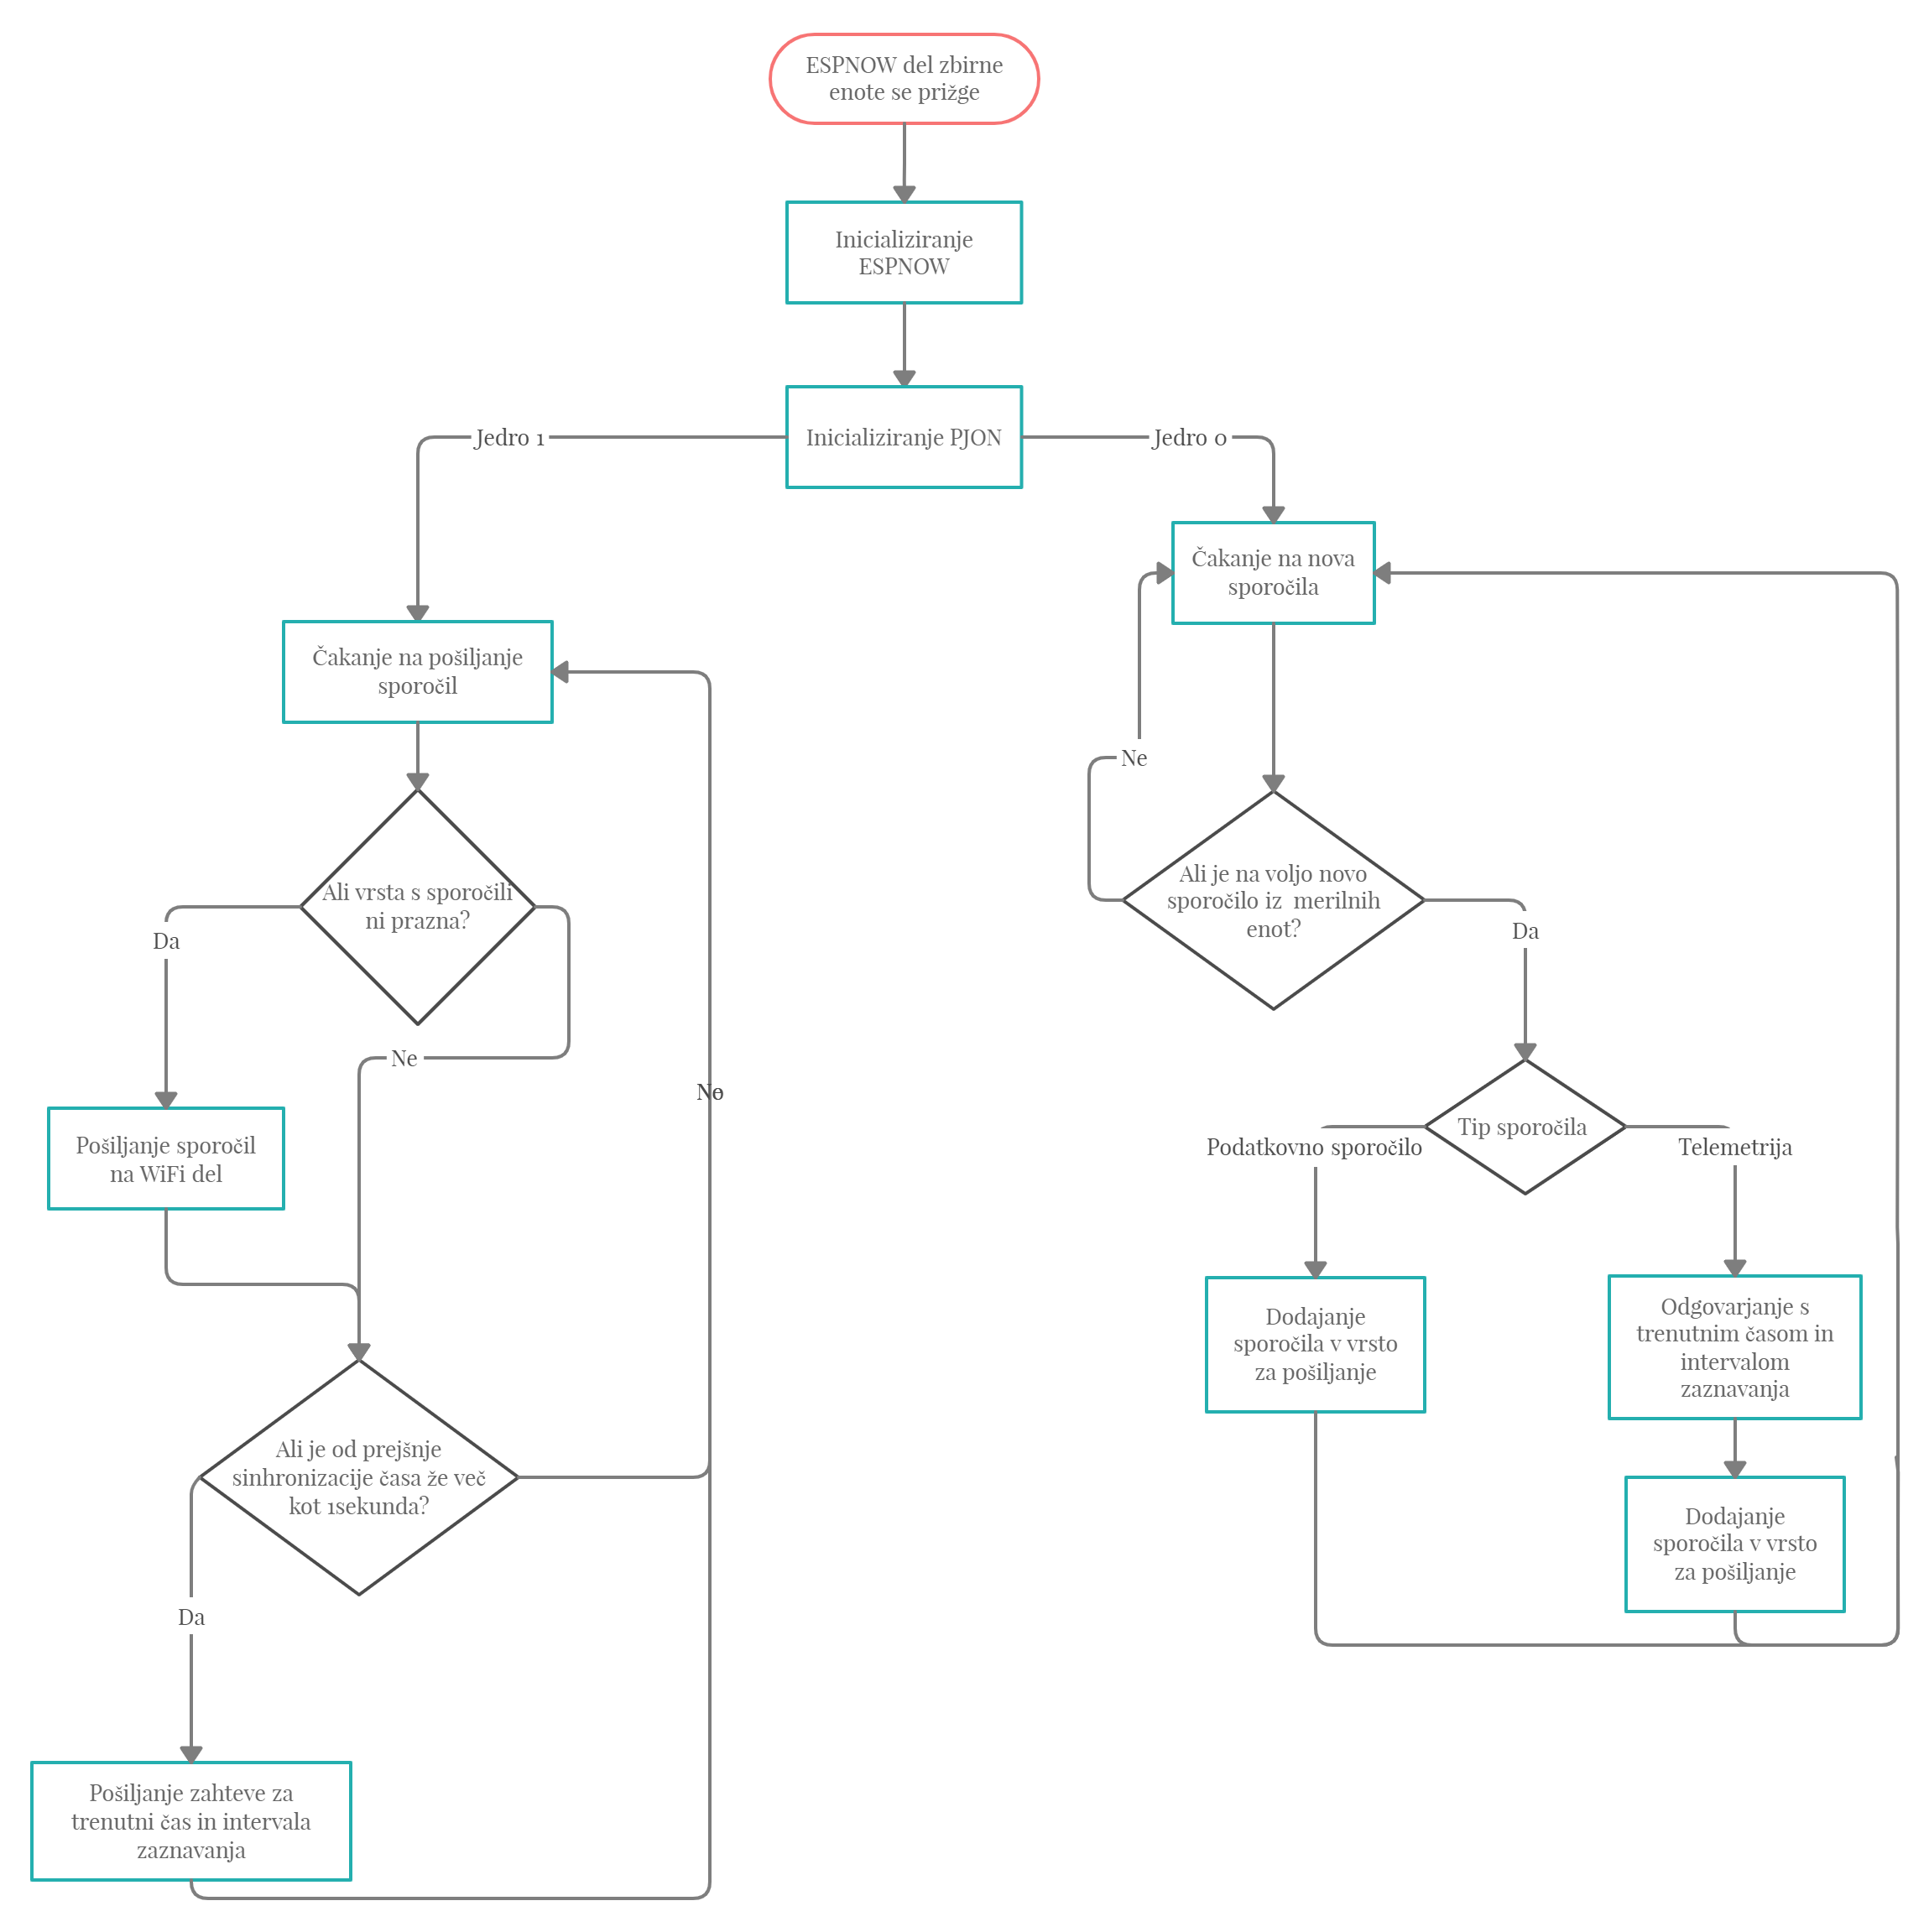
\includegraphics[width=\linewidth]{slikovno_gradivo/Zbirna enota koncept delovanjaESPNOW.png}
    \caption{TODO - daj v dve sliki to, da bo vsaka na svoji strani}
    \label{fig:INMP441}
\end{figure}


\begin{figure}[H]
    \centering
    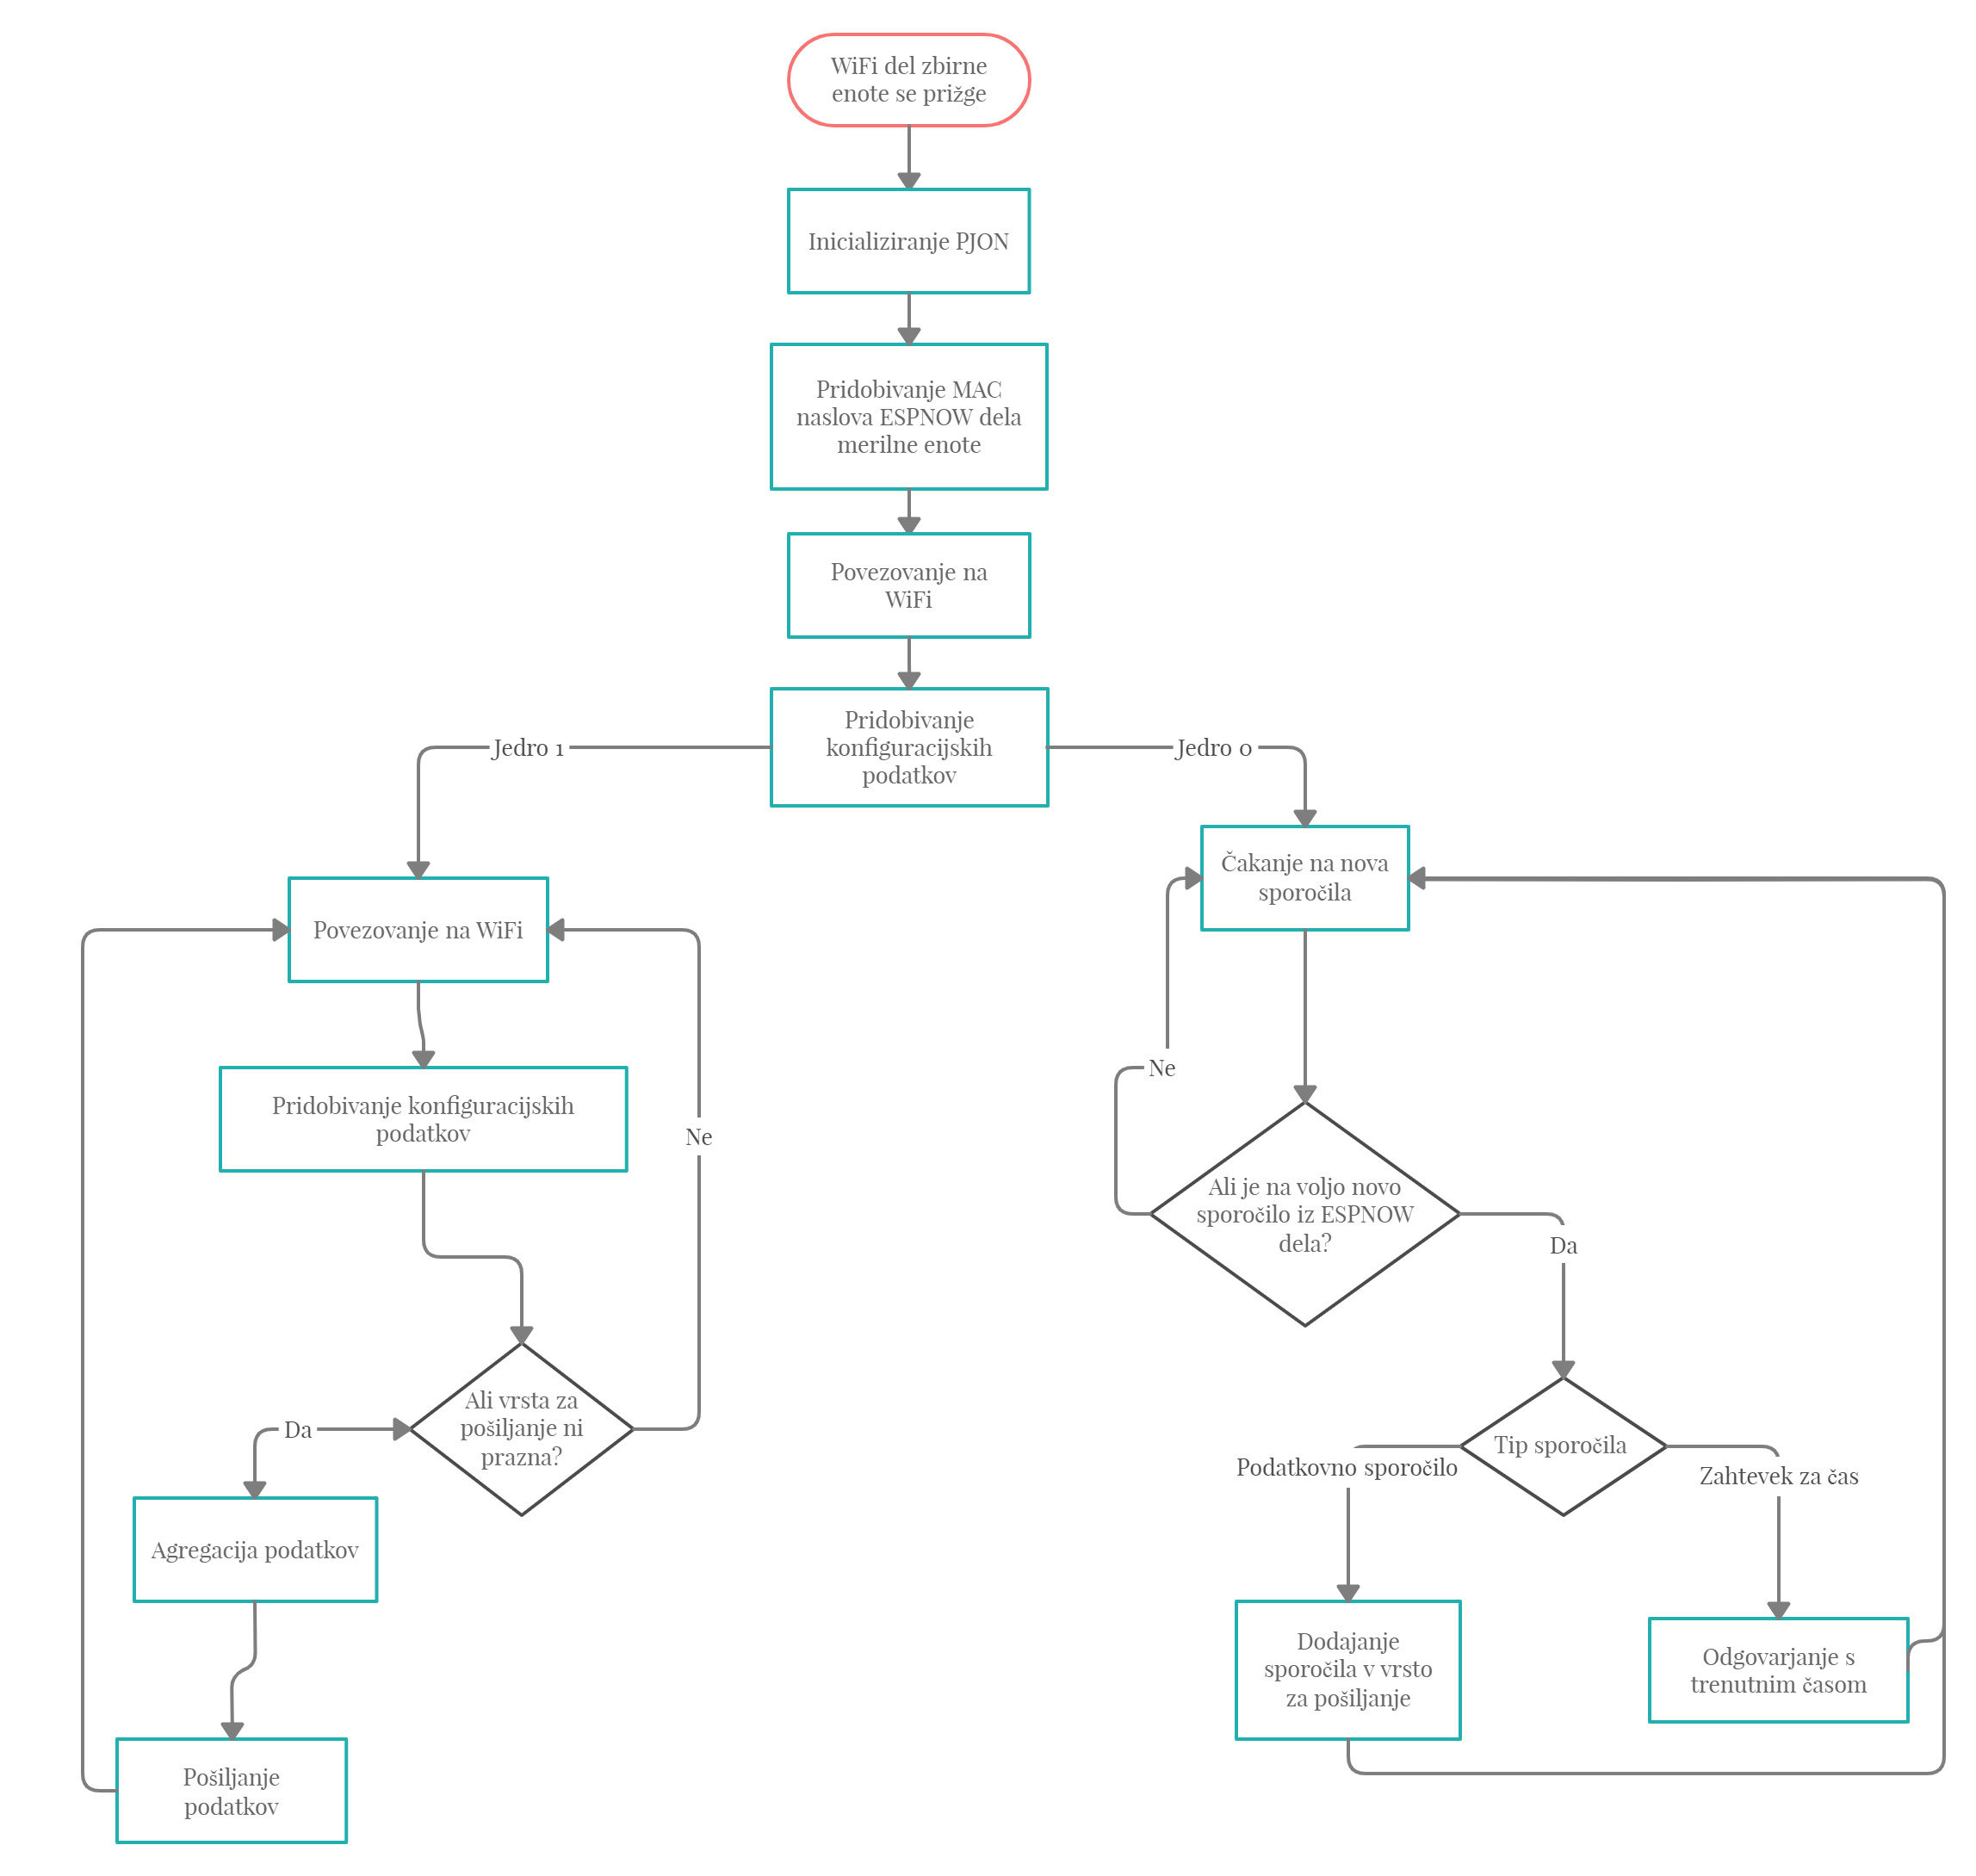
\includegraphics[width=\linewidth]{slikovno_gradivo/Zbirna enota koncept delovanjaWIFI.png}
    \caption{TODO - daj v dve sliki to, da bo vsaka na svoji strani}
    \label{fig:INMP441}
\end{figure}

* fotografija enote
\begin{figure}[H]
    \centering
    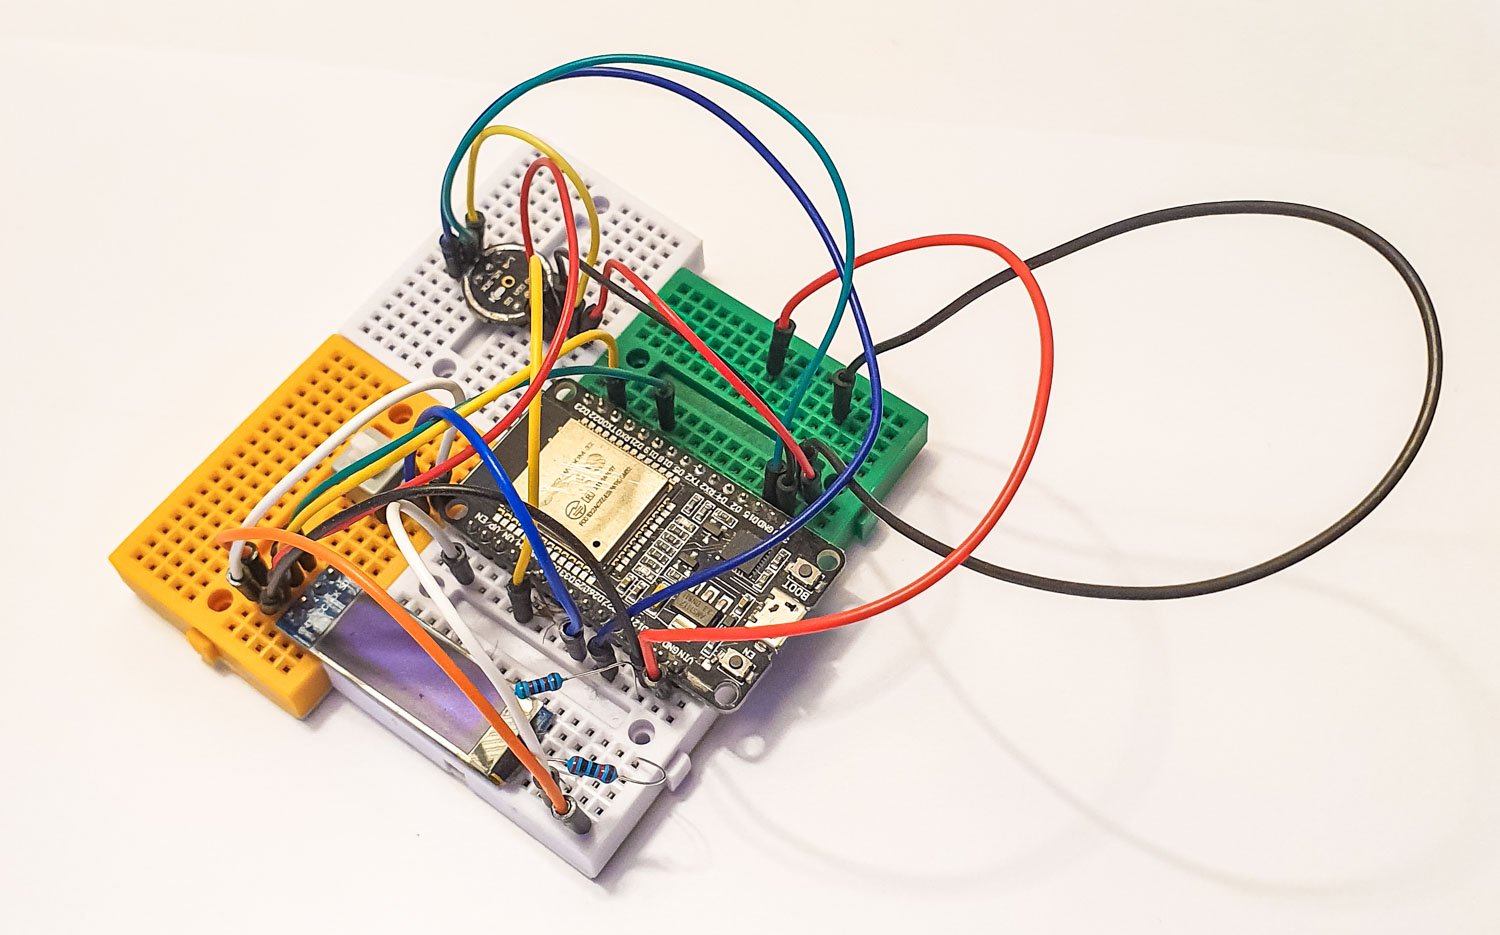
\includegraphics[width=\linewidth]{slikovno_gradivo/prototip_1.jpg}
    \caption{Caption}
    \label{fig:INMP441}
\end{figure}



\begin{figure}[H]
    \centering
    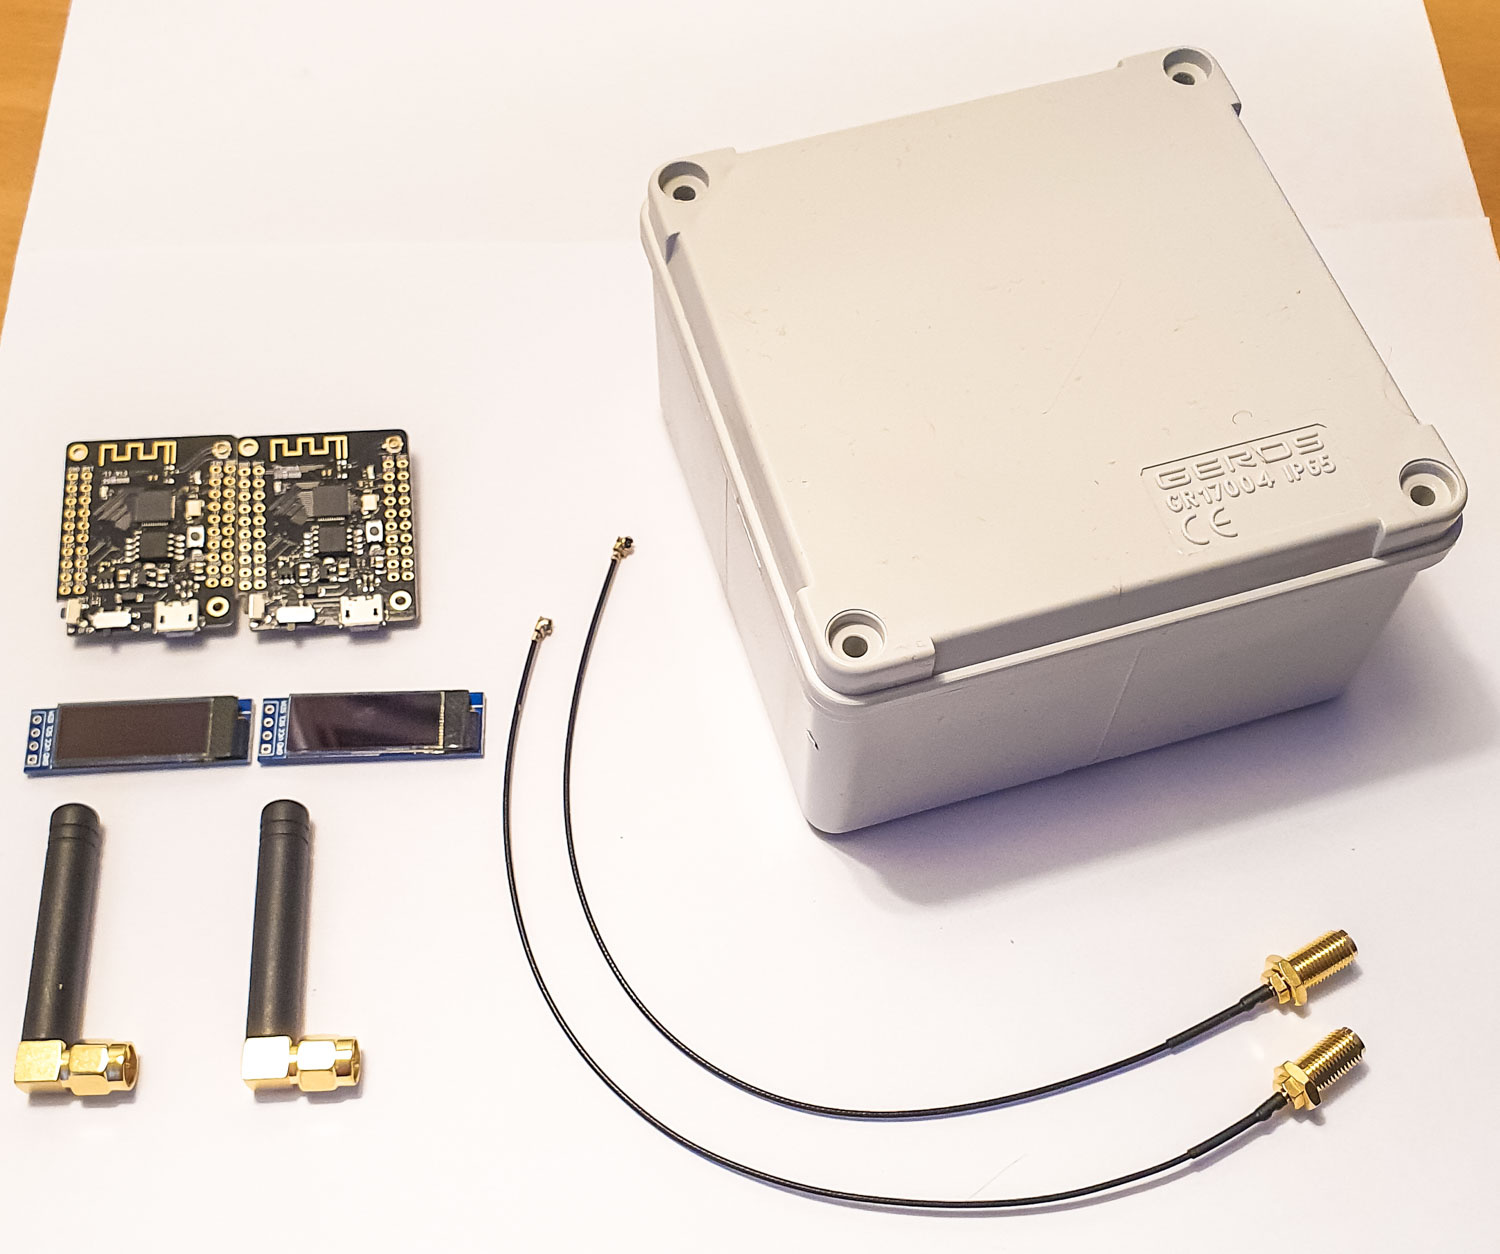
\includegraphics[width=\linewidth]{slikovno_gradivo/zbirna _enota_1.jpg}
    \caption{To je material za vsako zbirno enoto.}
    \label{fig:material_zbirna}
\end{figure}

Namen zbirne enote je posredovanje podatkov iz merilnih enot na strežnik in sinhronizacija časa na merilnih enotah. 
Ker ESPNOW protokol deluje samo med ESP napravami, smo pri zbirni enoti uporabili dva ista ESP32 čipa kot v merilni enoti.
Dva ESP32 čipa sta potrebna, ker isti čip ne more istočasno komunicirati prekko wifi in ESPNOW protokolov. Tako je en čip namenjen pošiljanju podatkov nastrežnik, drugi pa je namenjen prejemu podatkov iz merilnih enot. Med seboj komunicirata preko serijske UART povezave in protokola PJON, ki omogoča hitrejši razvoj zanesljivih podatkovnih povezav med mikrokontrolerji.
OLED zasloni prikazujejo statustiko pošiljanja in sprejemanja sporočil.


\section{Strežnik}
(konfigurator, API)

* shema podatkov v podatkovni bazi
\begin{figure}[H]
    \centering
    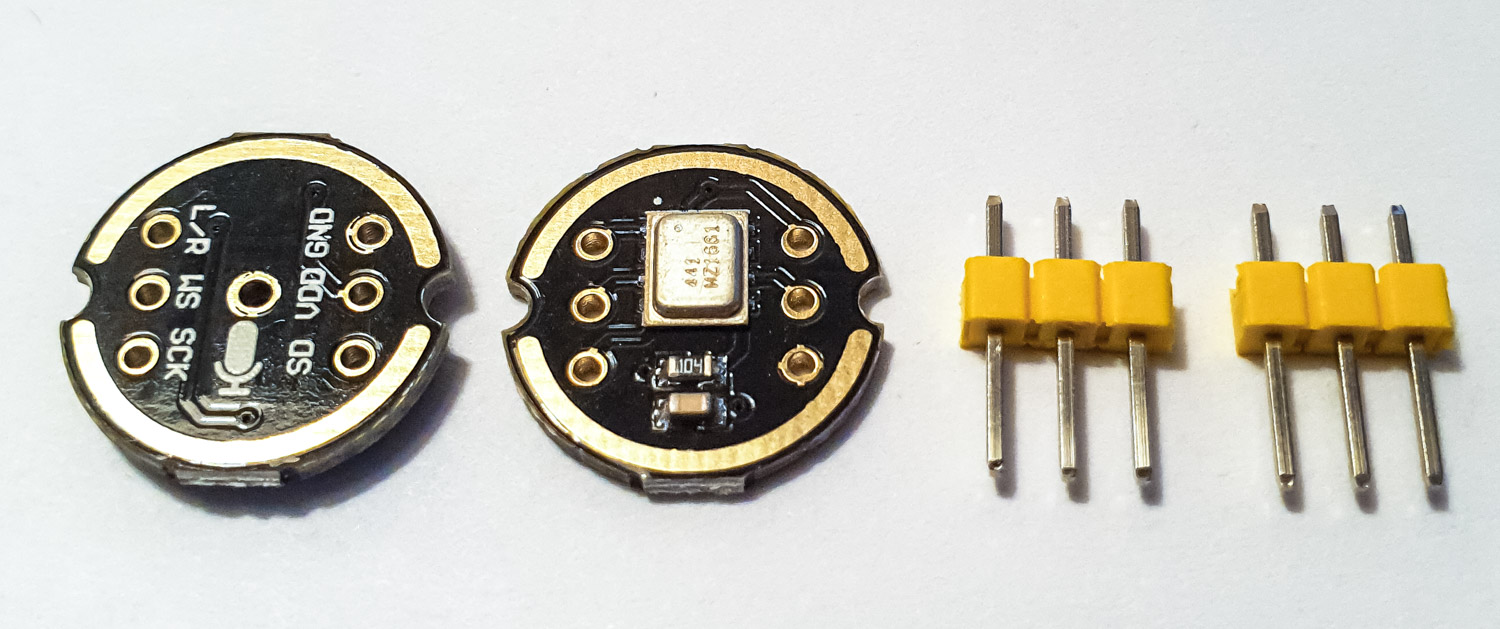
\includegraphics[width=\linewidth]{slikovno_gradivo/INMP441_1.jpg}
    \caption{Caption}
    \label{fig:INMP441}
\end{figure}

Strežniški del smo zasnovali tako, da navzven odpira api vmesnike. 
Zaledni del smo napisali v jeziku javascript in deluje v okolju NodeJS. Namestili smo ga na strežnik, ki je del biolaba. Na naslovu http://urbannoisesensing.biolab.si
Podatki so razdeljeni v več entitet, vsaka ima preko API rest vmesnika omogočene določene metode.
Sensor:
Hrani podatke o posamezni merilni enoti (mac, ime, trenutna lokacija, napetost baterije, trenutni deployment,...). Vmesnik omogoča pridobivanje osnovih podatkov o vseh senzorjih, polne podatke o določenem senzorju, registracijo novega senzorja z mac naslovom, pošiljanje zbranih podatkov o hrupu in pošiljanje podatkov o stanju baterije.

Gateway:
Hrani podatke o zbirni enoti (mac, ime, wifi gesla in imena, trenutni deployment). Vmesnik omogoča pridovianje osnovnih podatkov o vseh zbirnih enotah, pridobivanje vseh podatkov o posamezni enoti in registracijo nove enote z mac naslovom. 

Deployment:
Hrani podatke o deploymentih (ime, opis, katere merilne enote so del tega in kje so bile, katere zbirne enote so del tega, časovni okvri zajetih podatkov, število zajetih podatkov, trenutno stanje deploymenta). Vmesnik omogoča dodajanje novega deploymenta, začetek zbiranja podatkov z določenim deploymentom, končanje zbiranja podatkov, pridobivanje osnovnih podatkov o vseh deploymentih, pridobivanje vseh podatkov o specifičem deploymentu.  

Data:
Hrani zbrane podatke o hrupu (senzor, lokacija, začetni čas, končni čas, število meritev v tem dokumentu, meritve s svojimi atributi). Podatki so strukturirani v razdelke, ki so omejeni glede na število zbranih podatkov. Takšna razdelitev podatkov v skupine omogoča hitrejše iskanje po podatkih in zmanjšuje zmedo. Vmesnik omogoča več zanimivih agregacij podatkov. Recimo zadnjih n meritev iz vsake merilne enote, podatki ki so bili zbrani v zadnjih n sekundah, vsi zbrani podatki v določenem časovnem obdobju, podatki iz n najbolj razgibanih poljubnih časovnih intervalov.


\section{Poraba energije}



\begin{figure}[H]
    \centering
    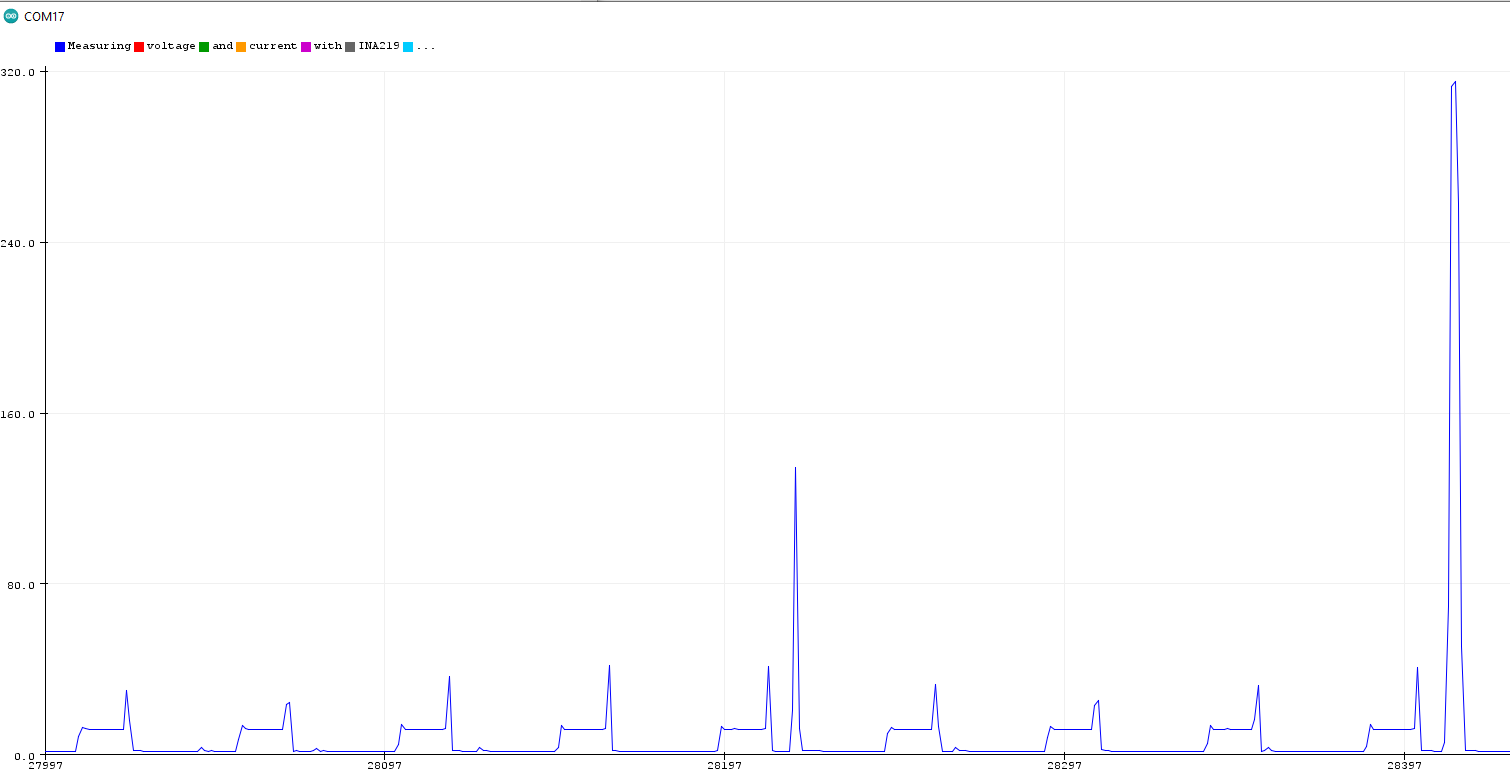
\includegraphics[width=\linewidth]{slikovno_gradivo/poraba-graf1.png}
    \caption{Na grafu porabe se jasno vidijo zaznavanja zvoka vsako sekundo in pošiljanja podatkov. Manjši vrh se ujema s pridobivanjem podatkov o času in intervalu, večji vrrh pa pošiljanje podatkov.}
    \label{fig:poraba1}
\end{figure}

\begin{figure}[H]
    \centering
    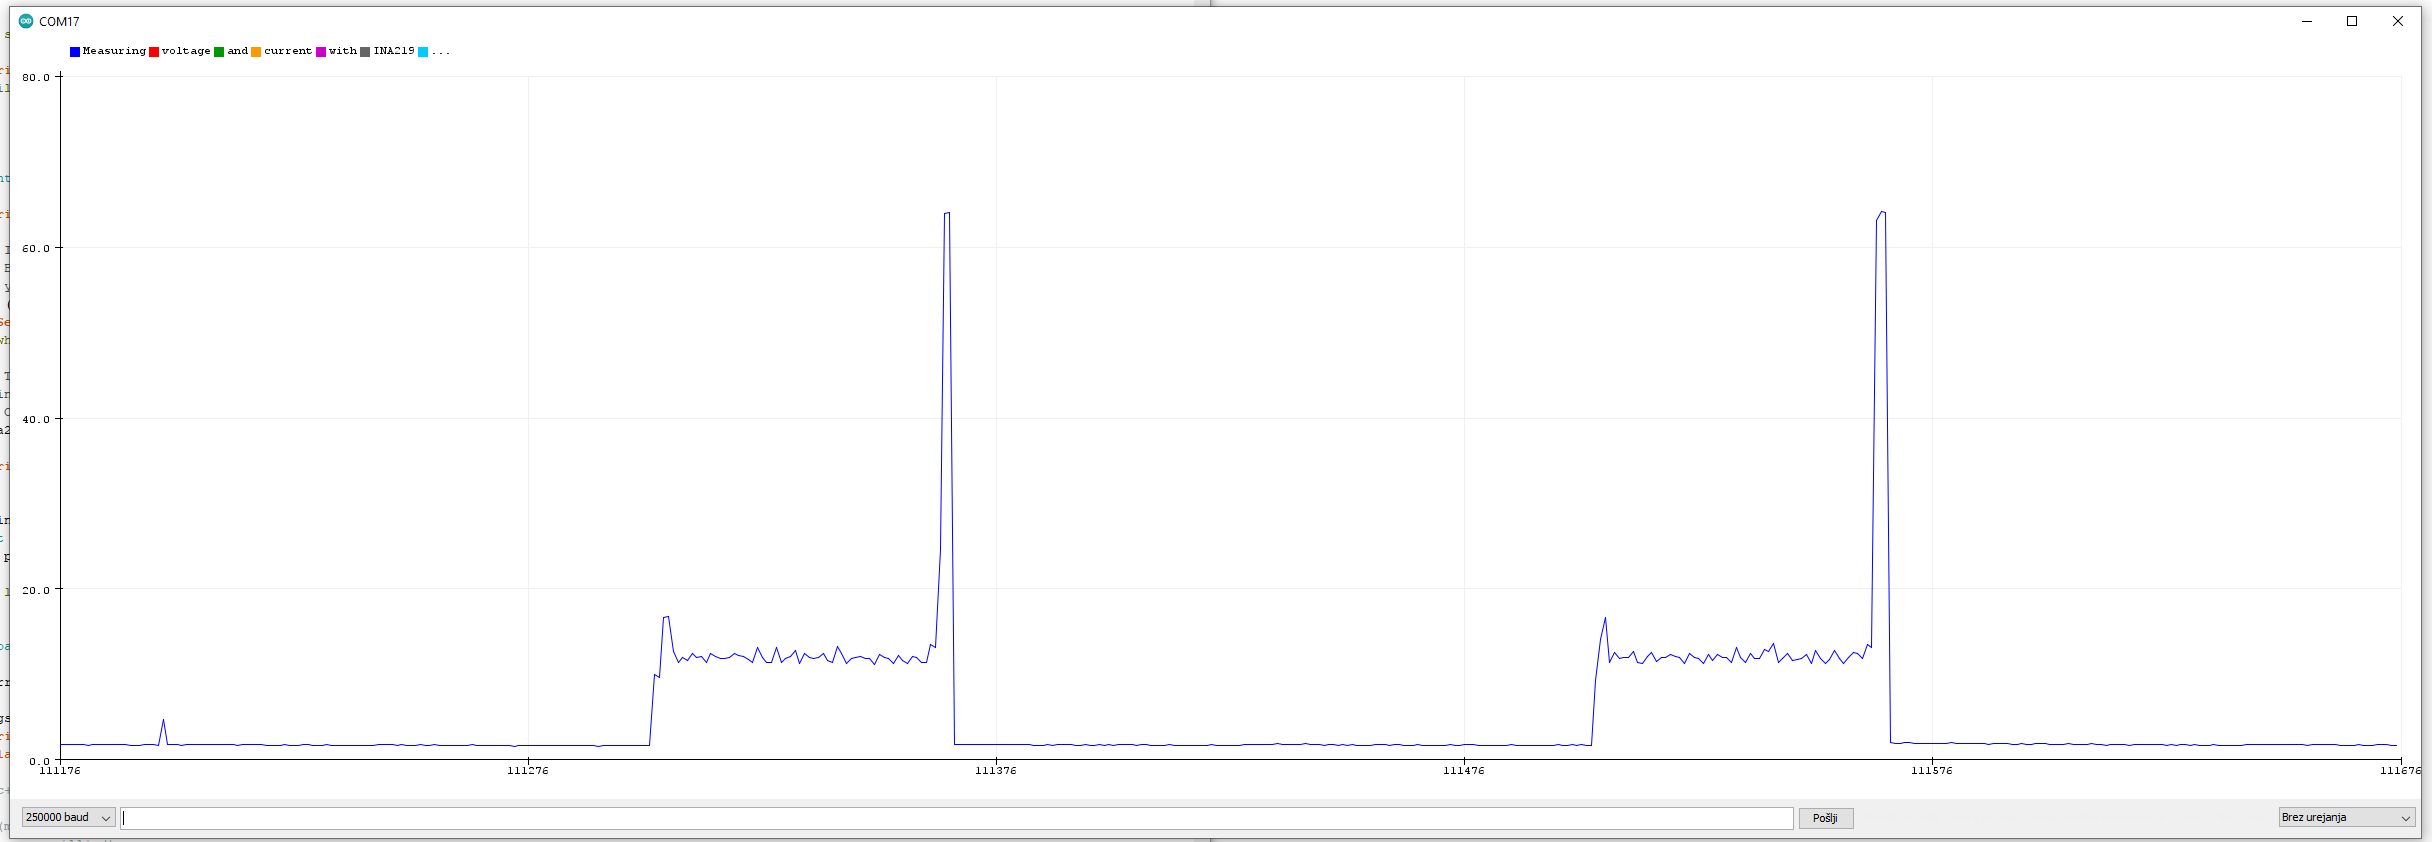
\includegraphics[width=\linewidth]{slikovno_gradivo/poraba-graf2.png}
    \caption{Na grafu porabe so jasno razvidni različni deli običajnega zaznavnega cikla. Enota najprej približno 700ms spi, kar se ujema z zelo nizko porabo. Sledi pridobivanje podatkov o zvoku, ki traja približno 250ms in ima zaradi nizke frekvence procesorja majhno porabo. Na koncu sledi obdelava podatkov, ki se zgodi pri največji hitrosti in korelira z vrhom, ki traja le nekaj milisekund.}
    \label{fig:poraba2}
\end{figure}

\begin{figure}[H]
    \centering
    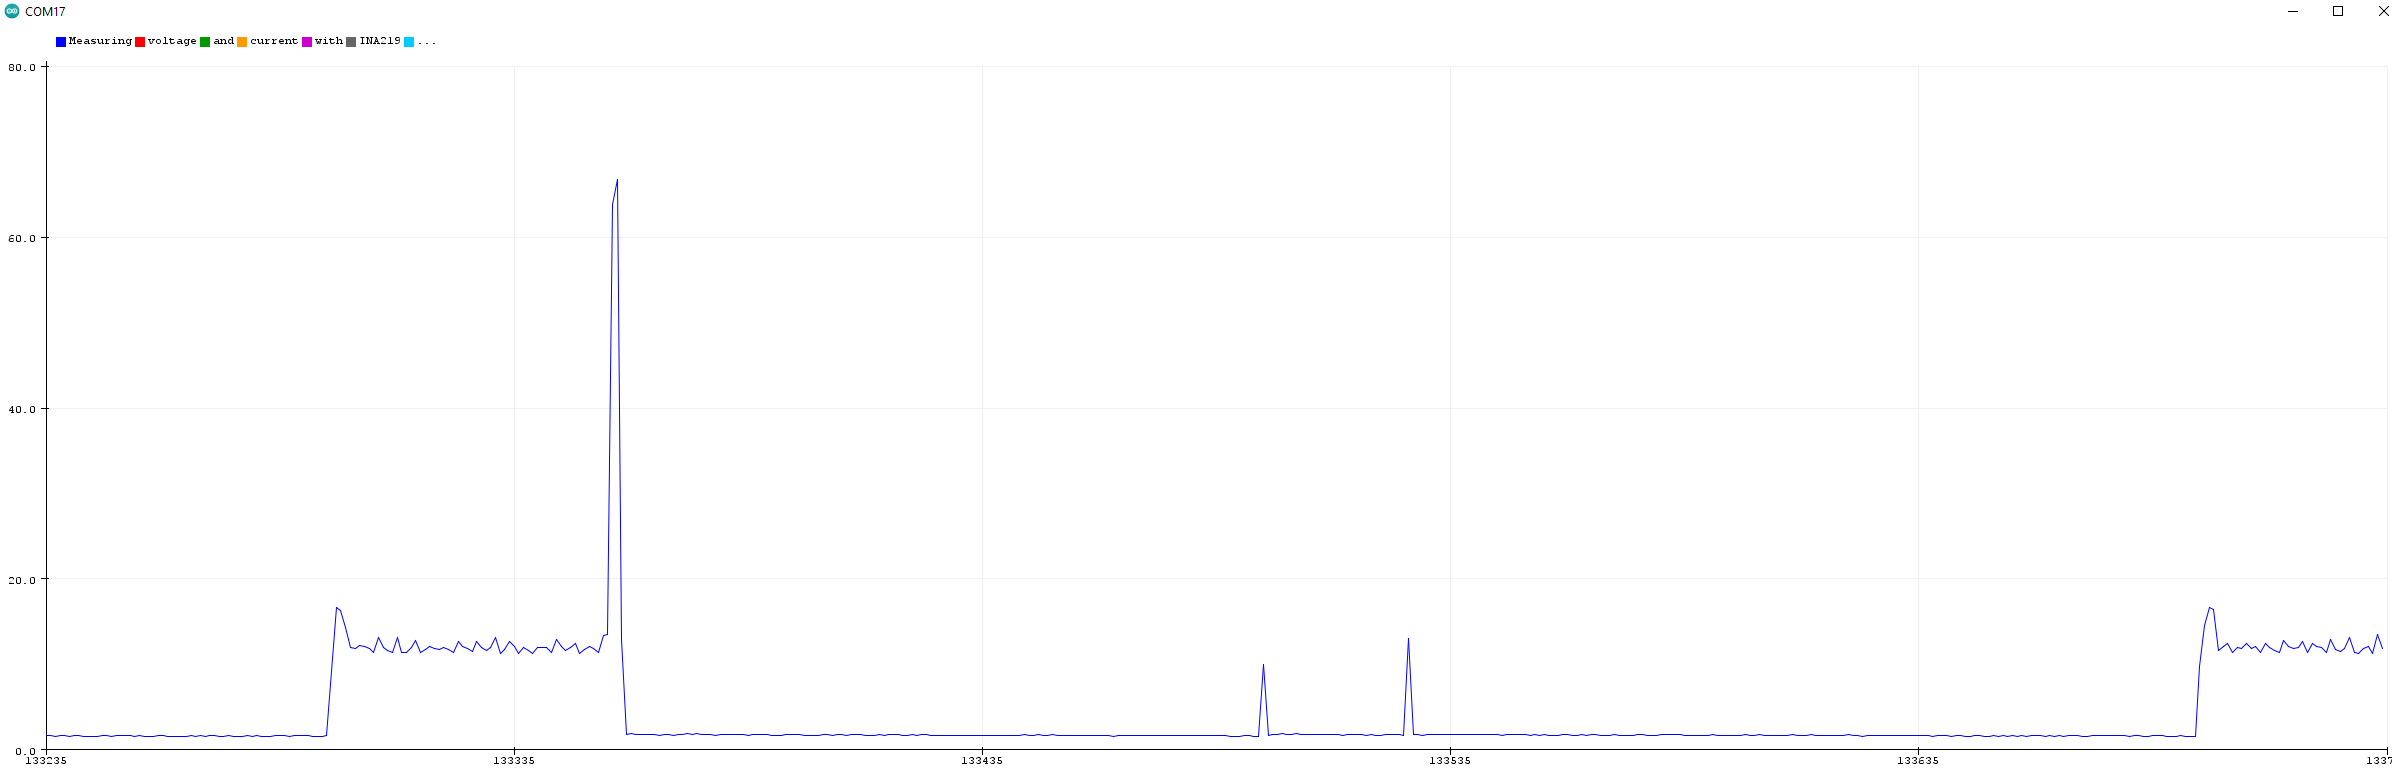
\includegraphics[width=\linewidth]{slikovno_gradivo/poraba-graf4.png}
    \caption{Na grafu porabe se vidi princip delovanja, ko je interval zaznavanja daljši od ene sekunde. Enota se eno sekundo po začetki prejšnnjega merjenja zbudi in preveri, ali je trenutno število sekund deljivo z intervalom merjenja. Ker ni, gre nazaj v način spanja. Nekaj milisekund kasneje, se enota spet zbudi in preveri če je že čas za pošiljanje ali usklajevanje časa.}
    \label{fig:poraba4}
\end{figure}



\begin{table}[H]
\begin{tabular}{l|l}
\multicolumn{1}{l}{Interval zaznavanja (s)} \vline & \multicolumn{1}{l}{Električni tok (mA)} \\ \hline
1                                             & 8.35                                     \\
2                                             & 5.65                                     \\
3                                             & 4.65                                     \\
4                                             & 4.14                                     \\
5                                             & 3.80                                     \\
6                                             & 3.60                                     \\
7                                             & 3.50                                     \\
8                                             & 3.35                                     \\
9                                             & 3.25                                     \\
10                                            & 3.15                                     \\
1000                                          & 2.61                                    
\end{tabular}
\caption{Povprečne porabe ob različnih intervalih merjenja hrupa.}
\label{tbl:poraba_tabela}

\end{table}


* koda kjer z dinamičnim nastavljanjem frekvence procesorjaa v merilni enoti in spanjem med merjenji dosežem nizko porabo
\begin{figure}[H]
    \centering
    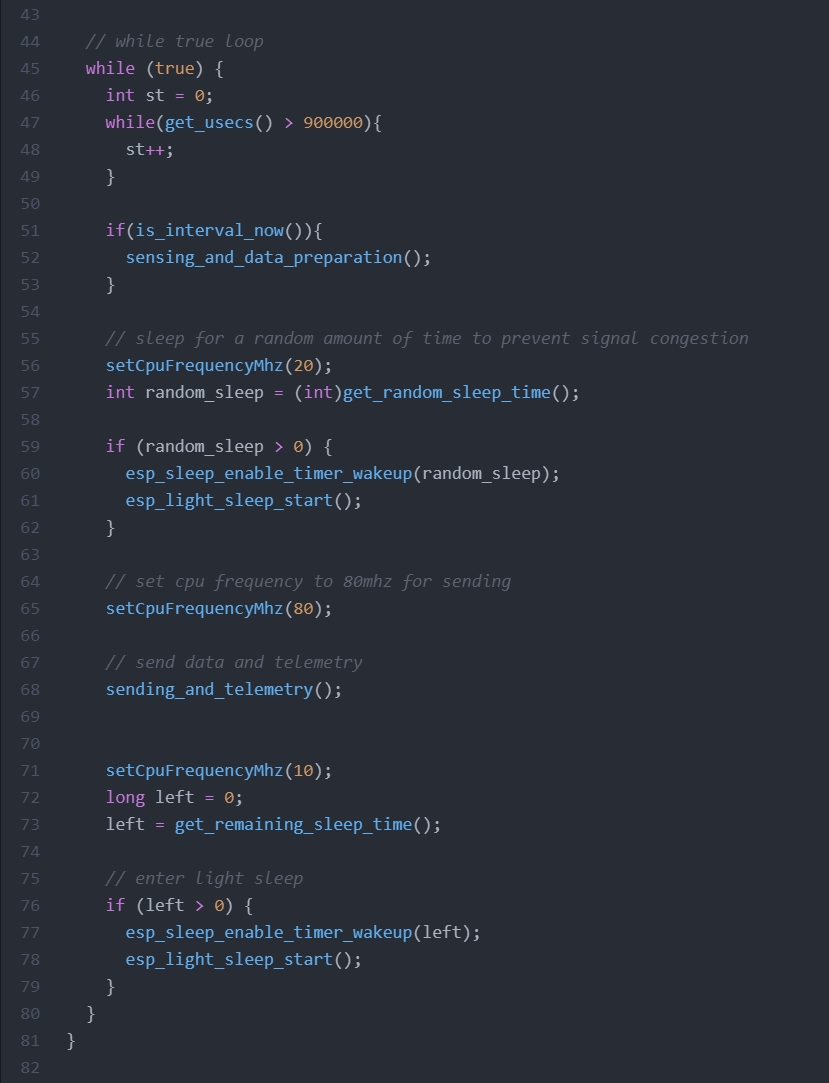
\includegraphics[width=\linewidth]{slikovno_gradivo/koda_whille_loop.png}
    \caption{Programska koda, ki koordinira celotno delovanje merilne enote v načinu merjenja. Jasno se vidi dinamično nastavljanje frekvence procesorja glede na trenutno aplikacijo za zmanjševanje porabe.}
    \label{fig:koda_while_loop}
\end{figure}

\section{Podatkovna analitika}

* posnetek zaslona widgeta
\begin{figure}[H]
    \centering
    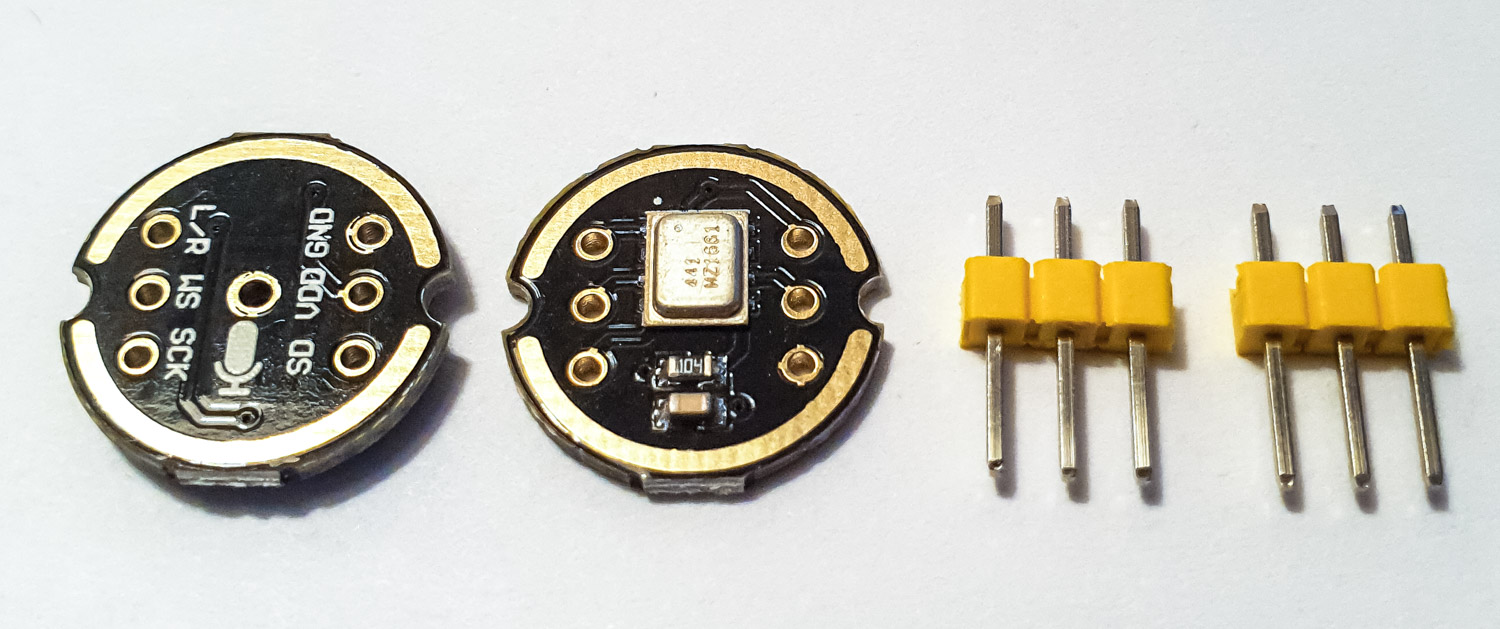
\includegraphics[width=\linewidth]{slikovno_gradivo/INMP441_1.jpg}
    \caption{Caption}
    \label{fig:INMP441}
\end{figure}


\begin{figure}[H]
    \centering
    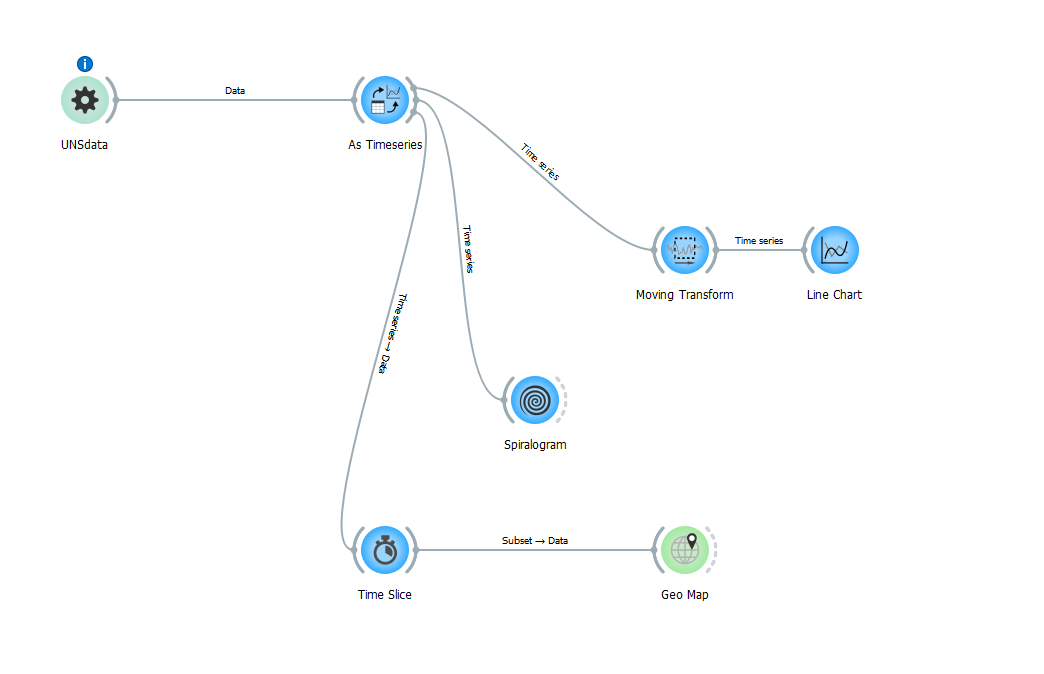
\includegraphics[width=\linewidth]{slikovno_gradivo/Primer workflowa Orange.png}
    \caption{Primer workflowa v programu Orange. Podatke pridobljene s pomočjo UNSdata widgeta, se najprej pretvori v časovno zaporedne podatke.}
    \label{fig:workflow_primer}
\end{figure}


Projekt, ki temelji na zbiranju podatkov je neuporaben brez dobrih orodij za podatkovno analitiko. Zato smo razvili widget za pridobivanje podtakov v kontekstu programa Orange. S tem smo uporabniku omogočili hitro in učinkovito analizo ažurnih podatkov. 
Widget omogoča uporabo vseh agregacij, ki jih ponuja entiteta data. Uporabnik ima na voljo dva načina priprave izhodnih podatkov. Izbira lahko med tensorji in matrico. 

 ** slike in primeri uporabe v Orange **
 
 
 \chapter{Uporabniška navodila}


\section{Polnenje merilnih enot}

Merilne enote napajajo li-ion polnilne baterije. Napolnjenost posamezne merilne enote se lahko preveri na strani ˝Sensors˝. Baterije so prazne pri napetosti približno 3.0V.

\begin{enumerate}
    \item Odstranite pokrov enote, ki je pritrjen s 4 vijaki.
    \item Z usb kablom povežite polnilno vezje z usb napajalnikom. Polnilno vezje je manjša ploščica z usb priključkom, montirana zraven mikorkontrolerja.
    \item Polnite dokler ne sveti zelena luč. Če je naprava med polnenjem prižgana v načinu nastavljanja, lahko preverite napolnjenost na strani ˝Sensors˝. Enota je napolnjena, ko napetost preseže 4.05V.
\end{enumerate}

\section{Prižiganje enot v različnih načinih}

Prva iteracija merilnih enot ima dve stikali, ki sta uporabljeni za prižiganje in izbiro načina delovanja. Naslednje bodo imele le eno stikalo in bo prižiganje in izbira delovanja trivialna operacija.







\section{Registracija merilne enote}

Pred uporabo enot v raziskavah, jih je treba registrirati v sistem.

\begin{enumerate}
    \item Poskrbite, da je napravam na voljo WiFi omrežje s povezavo na internet z SSID ˝UNSwifi˝ in deslom ˝uns12wifi34˝.
    \item Prižgite enote v način za nastavljanje.
    \item Počakajte, da se na ekranu izpiše ime enote.
\end{enumerate}


\section{Ustvarjanje raziskave}

Projekt je zasnovan na principu raziskav, ki so urejene v "deploymente".

\begin{enumerate}
    \item Registrirajte vse merilne in zbirne enote, ki bodo uporabljene v tej raziskavi.
    \item V spletnem vmesniku v zavihku ˝Deployments˝ pritisnite gumb ˝+˝, vpišite ime raziskave in pritisnite gumb ˝Create Deployment˝.
    \item Nadaljujte z urenjanjem raziskave.
\end{enumerate}


\section{Urejanje raziskave}

Pred začetkom zaznavanja je treba nastaviti in zagnati raziskavo.

\begin{enumerate}
    \item Ustvarite raziskavo, ali pa na strani ˝Deployments˝ v razdelku ˝Not yet deployed˝ izberite raziskavo, ki jo želite urediti.
    \item Raziskavi uredite ime in opis tako, da spremenite besedilo v vnosnih poljih in pritisnete gumb ˝Save changes˝.
    \item Merilne enote lahko raziskavi dodajate tako, da v razdelku ˝Sensors˝ s klikom na zemljevid na ustrezna mesta postavljate zaznamke.
    \begin{itemize}
        \item S klikom na zaznamek na zemljevidu odstranite enoto iz raziskave. 
        \item S klikom na ime postavljene merilne enote, se zaznamek na zemljevidu obarva.
        \end{itemize}
    \item Zbirno enoto lahko dodate v razdleku ˝Gateways˝ s klikom na ime izbrane zbirne enote.
    \item Gatewayu lahko dodate možnost povezovanja na dodatno WiFi dostopno točko tako, da vpišete podatke o tem omrežju v ustrezna polja v razdelku ˝Gateways˝.
    \item Raziskavo zaženete s klikom na gumb ˝DEPLOY˝.
    \item Raziskavo zbrišete s klikom na gumb ˝DELETE DEPLOYMENT˝.
    \end{enumerate}
    
    \section{Prenašanje podatkov na enote}
    
    Ko je raziskava zagnana, je treba konfiguracijske podatke prenesti na enote.
    
    \begin{enumerate}
        \item Poskrbite, da je napravam na voljo WiFi omrežje s povezavo na internet z SSID ˝UNSwifi˝ in deslom ˝uns12wifi34˝.
        \item Prižgite merilne enote v načinu za nastavljanje in počakajte, da se na ekranu izpiše MAC naslov zbirne enote.
        \item Povežite zbirno enoto na napajanje in počakajte, da se poveže na WiFi omrežje. 
        \item Ugasnite enote.
    \end{enumerate}
    
    
    \section{Postavljanje enot na lokacijo zaznavanja}
    
    Ko je raziskava zagnana in so podatki preneseni na enote, lahko postavite enote na lokacijo zaznavanja. 
    
    \begin{enumerate}
    \item Podkrbite, da so pokrovi vseh enot ustrezno pritrjeni in da so baterije merilnih enot ustrezno polne.
    \item Enote vsako posebej postavite na specificirane lokacije in jih prižgite v način za zaznavanje. Točne lokacije merilnih enot lahko preverite tako, da v spletnem vmesniku na strani ˝Deployments˝ v razdelku ˝Deployed˝ izberete trenutno raziskavo in v zavihku ˝Sensors˝ s klikom na posamezno ime enote na zemljevidu preverite, kje točno naj bi se posamezna enota nahajala. 
    \item Postavite in priklopite zbirno enoto v dosegu prej specificiranega WiFi omrežja.
    \end{enumerate}
    
    \section{Uravnavanje intervala zaznavanja}
    
    Privzeti interval zaznavanja je 1 sekunda. S povečevanjem intervala se podaljša doba delovanja baterij in zmanjša količina podatkov.
    
    \begin{enumerate}
        \item V spletnem vmesniku na strani ˝Deployments˝ v razdelku ˝Deployed˝ izberite trenutno raziskavo. 
        \item V razdelku ˝Sensing interval˝ v vpisno polje vpišite ustrezno dolžino intervala v sekundah.
        \item Pritisnite gumb ˝Save changes˝. 
    \end{enumerate}
    
    \section{Konec zaznavanja}
    
    Po končani raziskavi, je treba zaključiti "deployment".
    
    \begin{enumerate}
        \item V spletnem vmesniku na strani ˝Deployments˝ v razdelku ˝Deployed˝ izberite trenutno raziskavo. 
        \item Pritisnite gumb ˝FINISH SENSING˝. Če ni bilo opravljenih nič uspešnih meritev, je treba raziskavo izbrisati z gumbom ˝DELETE DEPLOYMENT˝.
    \end{enumerate}
    
    

\section{Podatkovna analitika}









Spletni vmesnik

    
    
 * posnetki zaslona frontenda pri nastavljanju
 \begin{figure}[H]
    \centering
    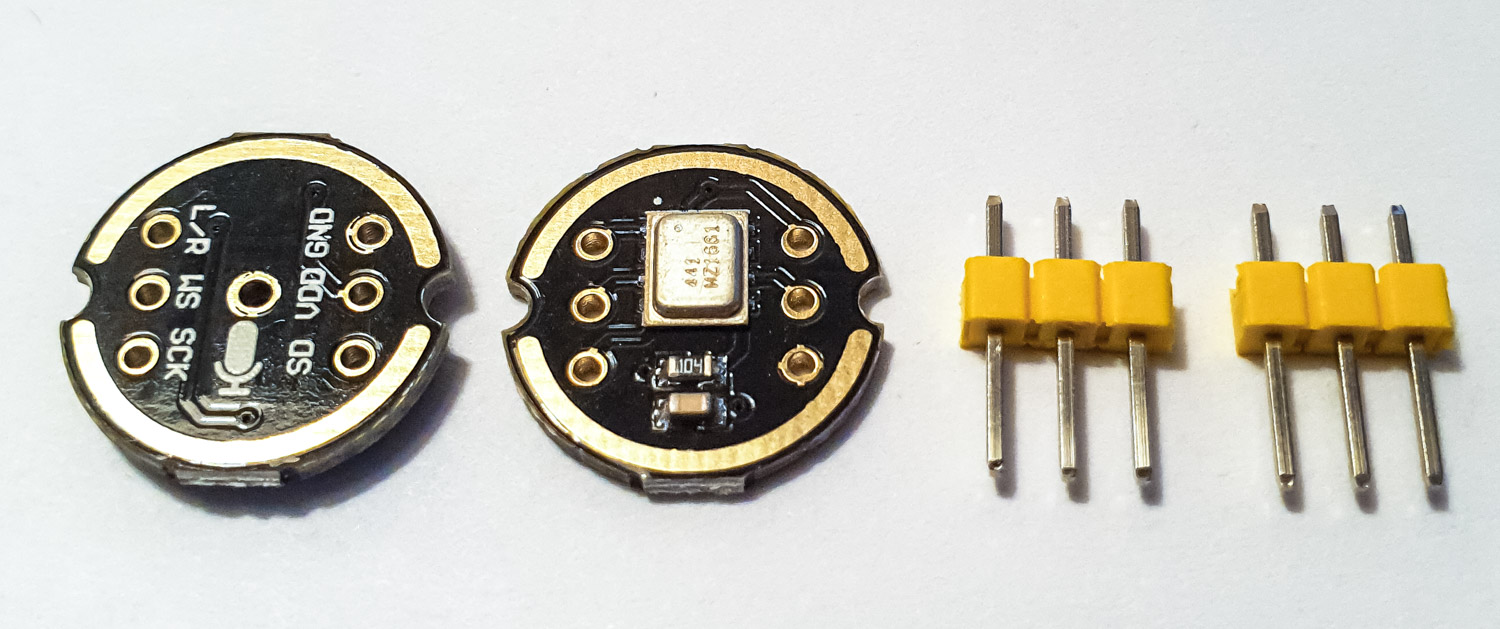
\includegraphics[width=\linewidth]{slikovno_gradivo/INMP441_1.jpg}
    \caption{Caption}
    \label{fig:INMP441}
\end{figure}
* fotografije zaslonov na merilnih in zbirnih enotah ob različnih fazah nastavljanja
 \begin{figure}[H]
    \centering
    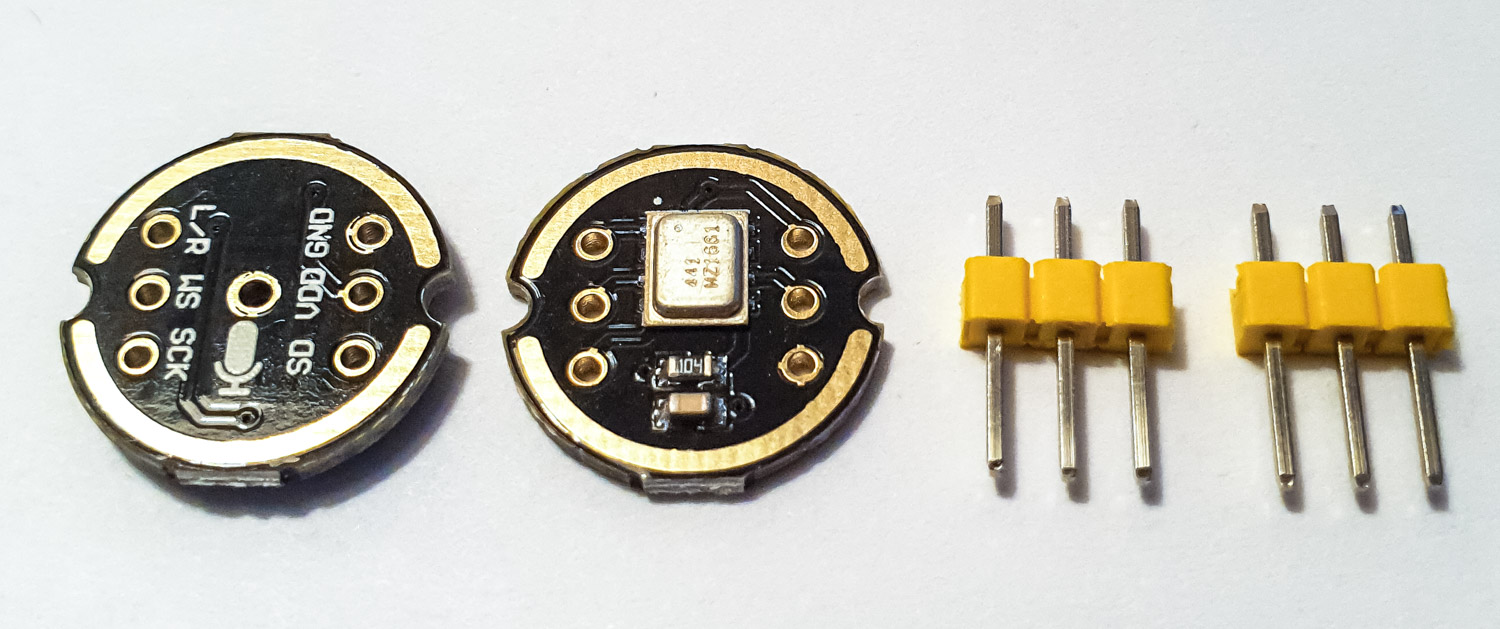
\includegraphics[width=\linewidth]{slikovno_gradivo/INMP441_1.jpg}
    \caption{Caption}
    \label{fig:INMP441}
\end{figure}
 

\chapter{Primera uporabe}
(motivacija, postavitev, rezultati, interpetacija - štirje odstavki)

Na vse senzorske in zbirne enote je nameščena enaka koda. Ko se enote prvič prižge v načinu nastavljanja, se povežejo na zaledni del in pošljejo svoj unikaten mac naslov in se tako registrirajo. Ob tem se generira naključno ime za posamezno enoto in uporabnik jo lahko nastavi za delo z eno raziskavo. 

\section{Kosilnica}

* posnetek zemljevida z lokacijami merilnih enot (in vrisano potjo košenja - mogoče če bom pri volji)
\begin{figure}[H]
    \centering
    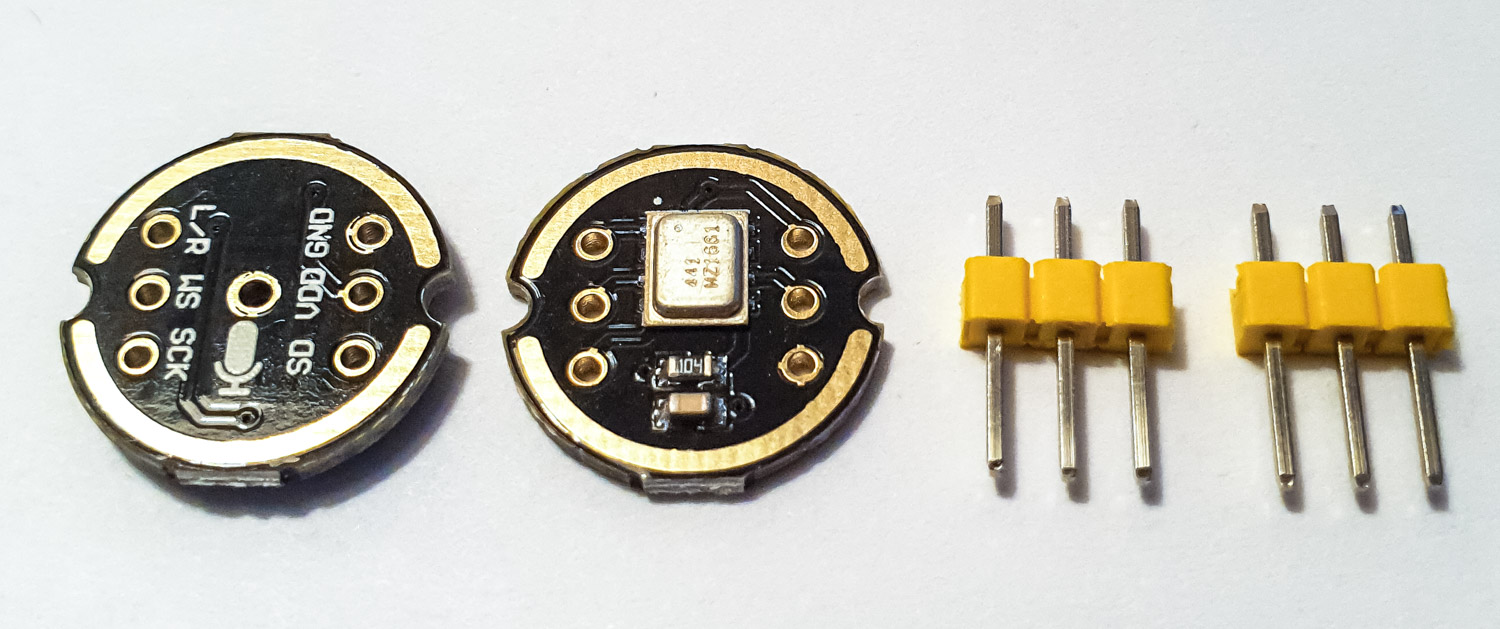
\includegraphics[width=\linewidth]{slikovno_gradivo/INMP441_1.jpg}
    \caption{Caption}
    \label{fig:INMP441}
\end{figure}


\begin{figure}[H]
    \centering
    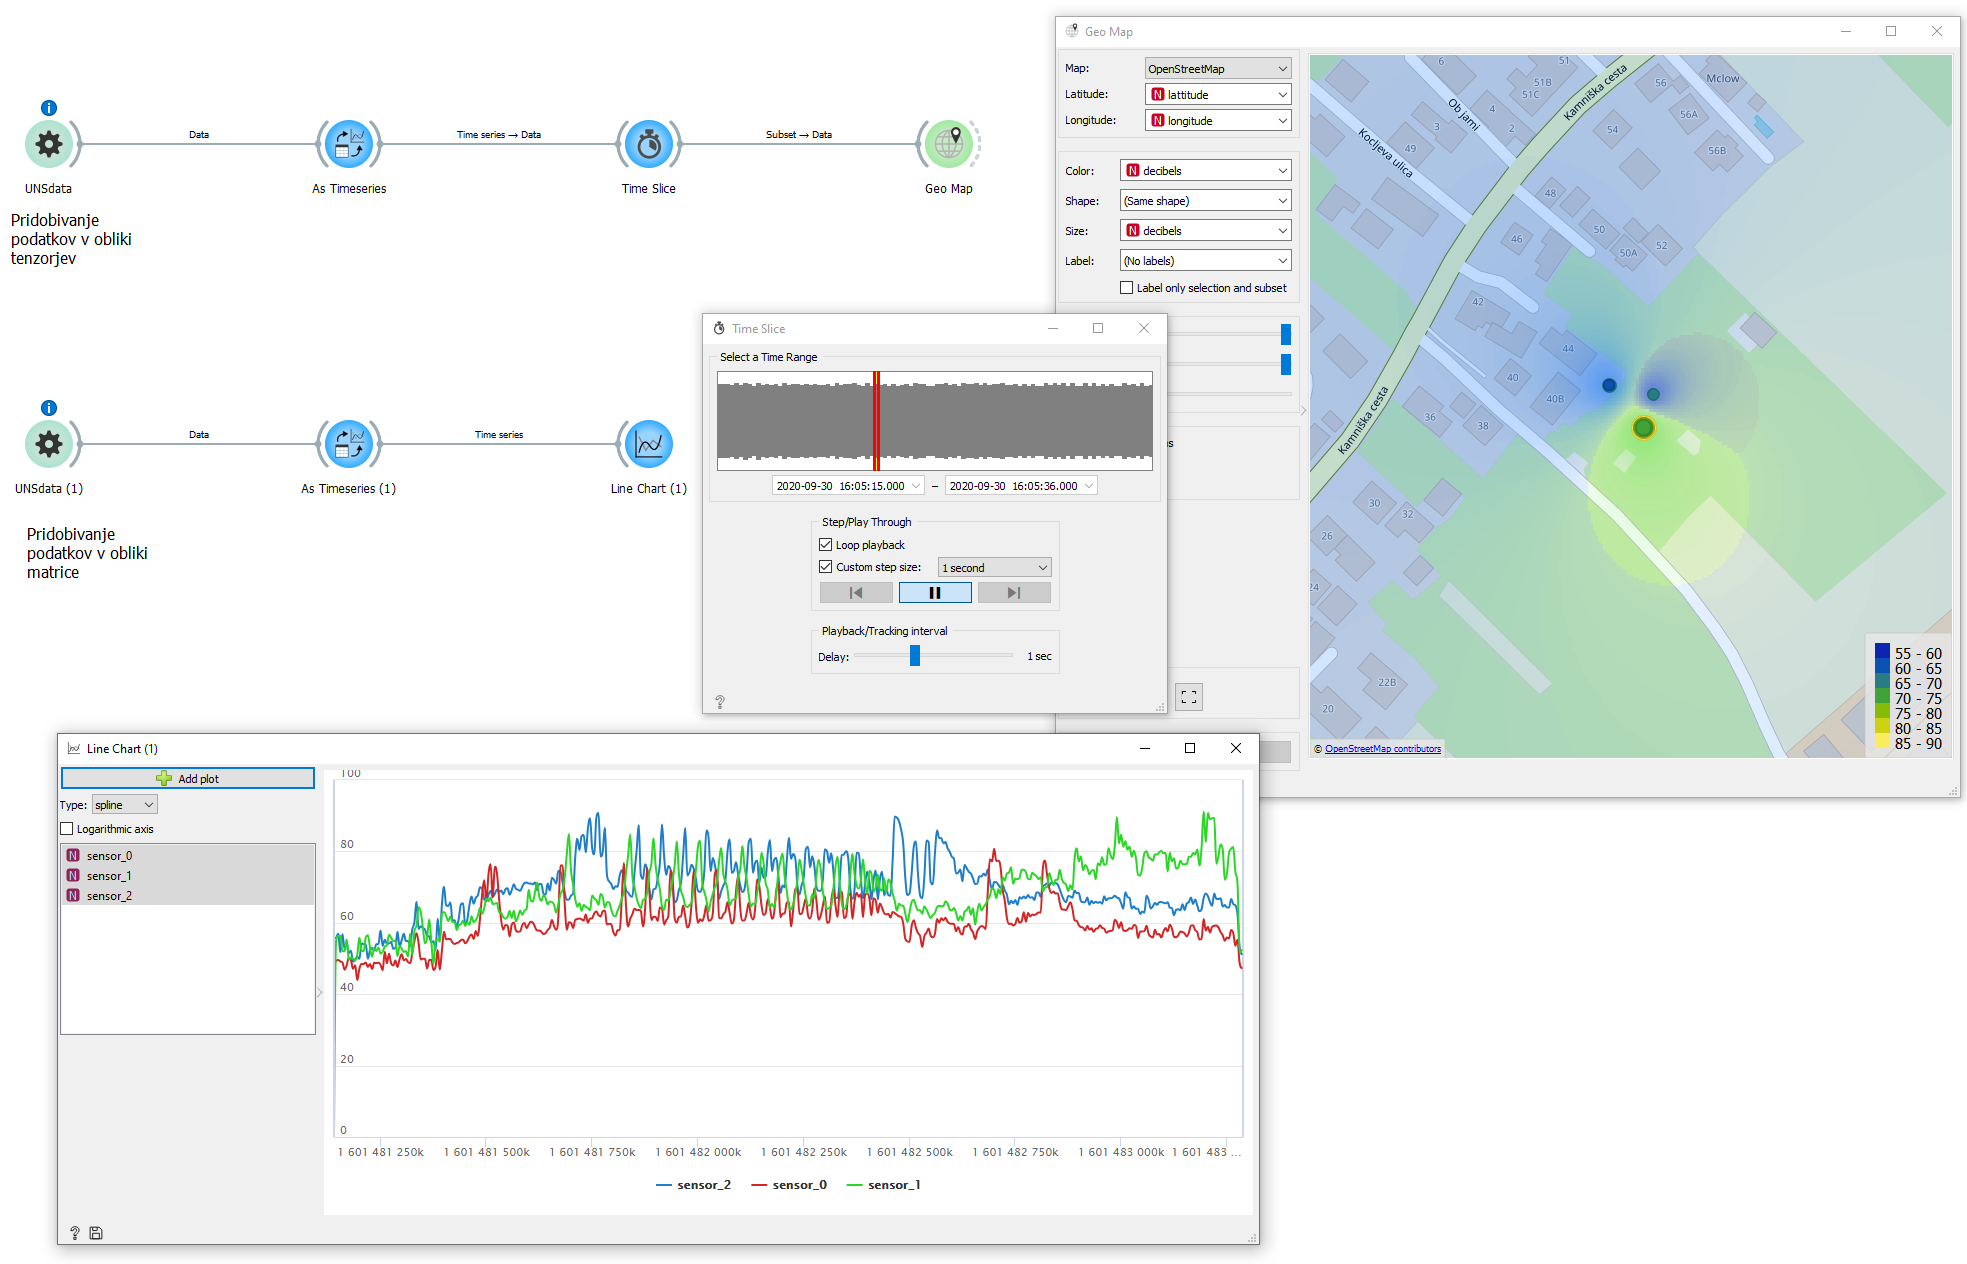
\includegraphics[width=\linewidth]{slikovno_gradivo/kosilnica-workflow.png}
    \caption{Pri priemru kosilnice smo raziskovali kako natančno lahko določimo gibanje izvira hrupa glede na  izmerjeno glasnost na vsakem senzorju. Podatke smo za prikaz na mapi izvozili kot tenzorje in jih potem s pomočjo geografskih orodij prikazali na zemljeidu dejanske lokacije. Za prikaz grafa po času pa smo podatke izvozili kot matrico in jih tako prikazali na grafu.}
    \label{fig:workflow_kosilnica}
\end{figure}


\begin{figure}[H]
    \centering
    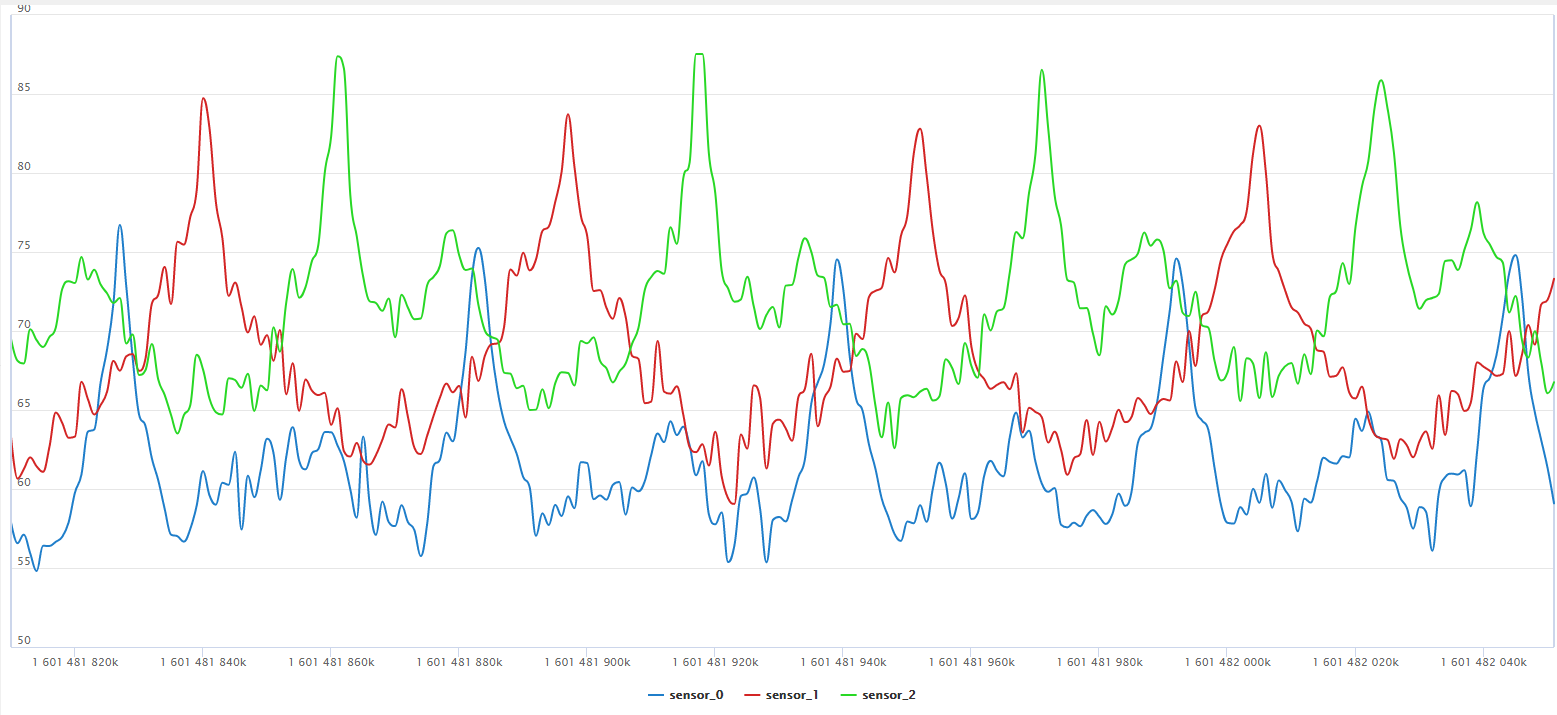
\includegraphics[width=\linewidth]{slikovno_gradivo/kosilnica-graf.png}
    \caption{Na grafu vseh meritev po času in senzorju, se jasno vidi, kako se je kosilnica približevala in oddaljevala vsakemu od senzorjev. Ker smo senzorje postavili na rob travnika, kosilnica pa se je v spirali gibala proti sredini, je možno opaziti, da so vrhovi po času vedno manjši, ker je razdalja med kosilnico in senzorjem z zmanjševanjem premera kroga vedno večja.}
    \label{fig:graf _kosilnica}
\end{figure}


\begin{figure}[H]
    \centering
    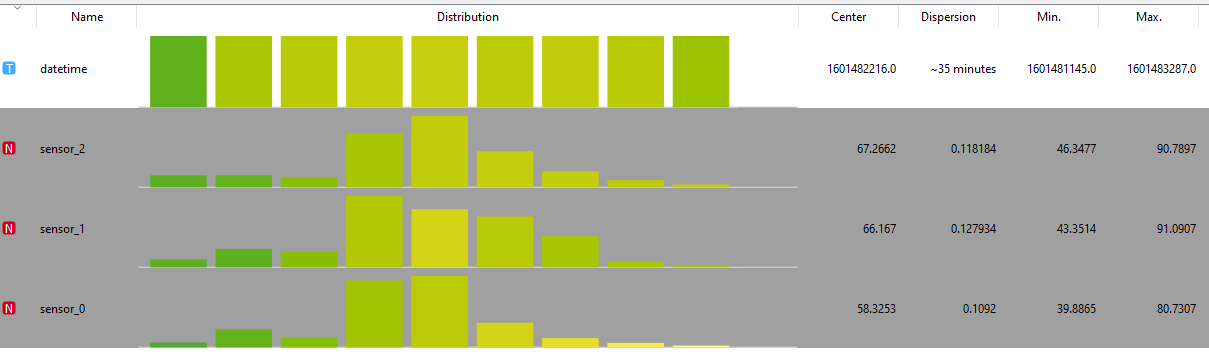
\includegraphics[width=\linewidth]{slikovno_gradivo/kosilnica-tabela-monmax.png}
    \caption{V tabeli z osnovnimi informacijami o podatkih je možno opaziti minimalne in maksimalne vrednosti glede na senzor.}
    \label{fig:tabela_kosilnica}
\end{figure}

(motivacija, postavitev, rezultati, interpetacija - štirje odstavki)

S tem poskisom smo želeli opazovati možnost spremljanja lokacije vira hrupa. Merilne enote smo pred košenjem postavili ob rob travnika, da se jasno vidijo oscilacije hrupa, ki ga je proizvedla kosilnica. 
Jasno se vidi, kdaj je bila kosilnica najbližje posamezni merilni enoti.


\section{Glasnost na faksu}

* posnetek zaslona zemljevida z lokacijami merilnih enot
\begin{figure}[H]
    \centering
    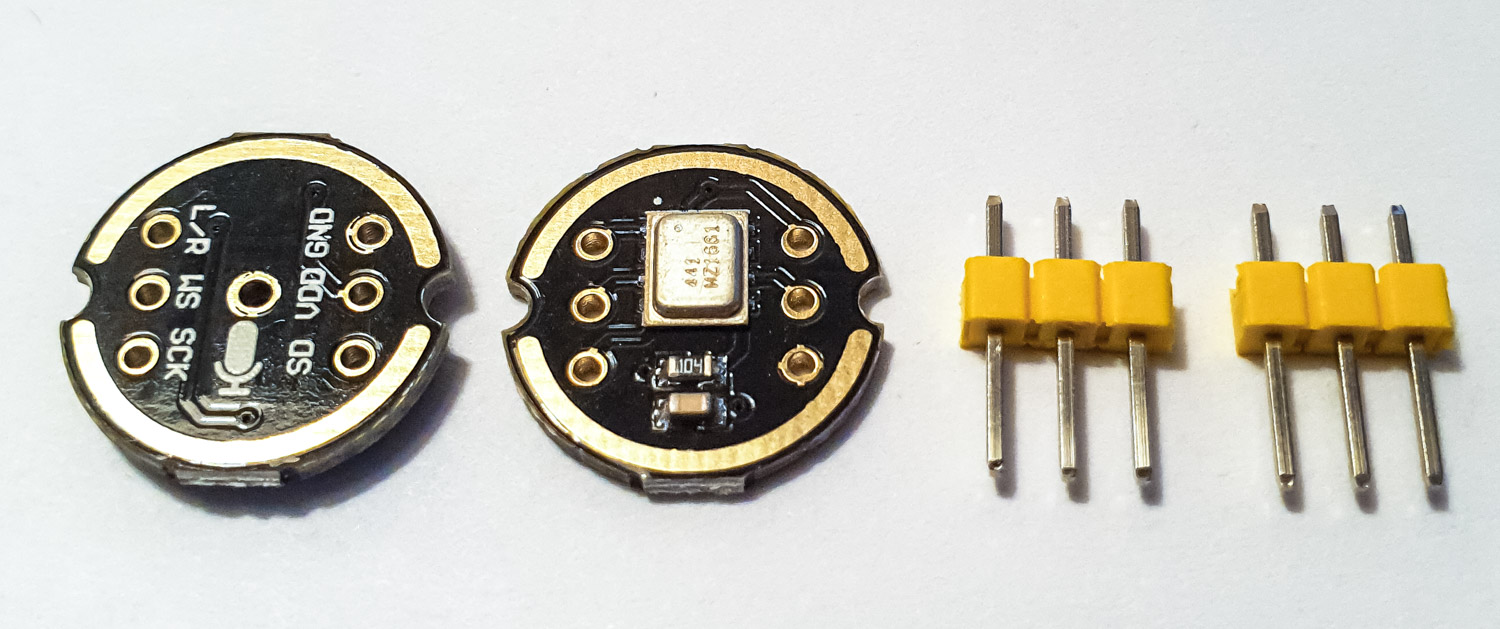
\includegraphics[width=\linewidth]{slikovno_gradivo/INMP441_1.jpg}
    \caption{Caption}
    \label{fig:INMP441}
\end{figure}
* posnetek zaslona workflowa v Orange
\begin{figure}[H]
    \centering
    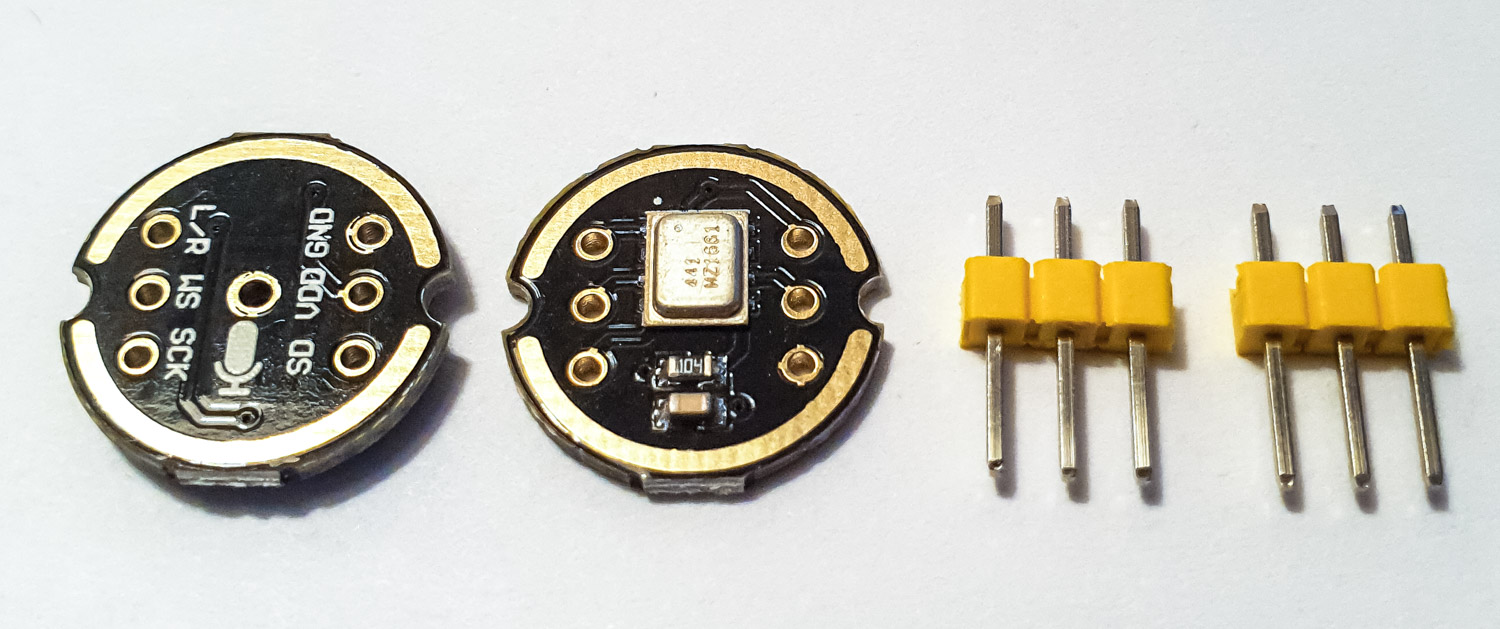
\includegraphics[width=\linewidth]{slikovno_gradivo/INMP441_1.jpg}
    \caption{Caption}
    \label{fig:INMP441}
\end{figure}
* zglajen graf po meritvah
\begin{figure}[H]
    \centering
    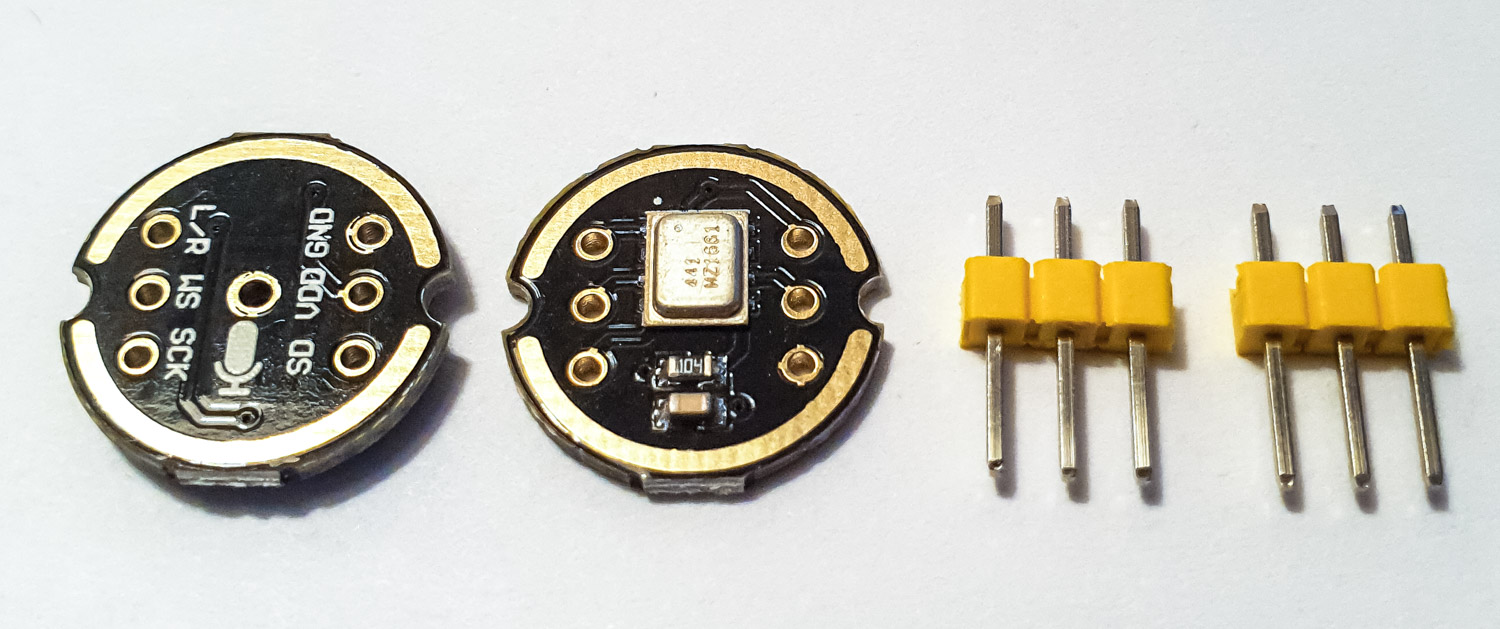
\includegraphics[width=\linewidth]{slikovno_gradivo/INMP441_1.jpg}
    \caption{Caption}
    \label{fig:INMP441}
\end{figure}
* spiralogram za prikaz periodnega ponavljanja vzorcev v glasnosti
\begin{figure}[H]
    \centering
    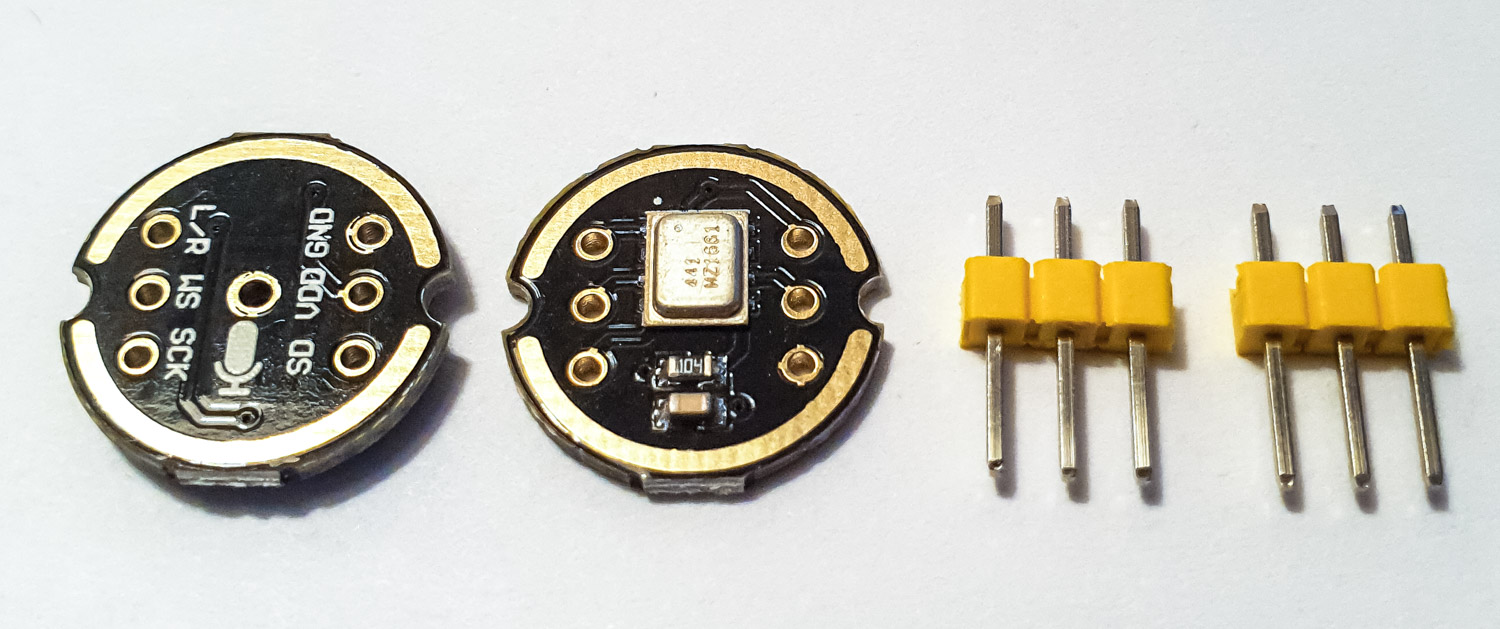
\includegraphics[width=\linewidth]{slikovno_gradivo/INMP441_1.jpg}
    \caption{Caption}
    \label{fig:INMP441}
\end{figure}

(motivacija, postavitev, rezultati, interpetacija - štirje odstavki)

\chapter{Zaključek}
(ni podpoglavij, samo trije odstavki)
- sklepne misli (kaj je bila naša naloga)
- rezultat (kako smo jo uspešno rešili)
- kaj še ostane (če bi imel čas in denar, kaj bi še lahko naredil iz tega, urbanisti, ...)



\newpage %dodaj po potrebi, da bo številka strani za Literaturo v Kazalu pravilna!
\ \\
\clearpage
\addcontentsline{toc}{chapter}{Literatura}
\bibliographystyle{plain}
\bibliography{literatura}


\end{document}

